% #----------------------------------------------#
% |   Autor Plantilla: Eduardo Cañete Carmona    |
% |   Fecha creación: 01/07/2019                 |
% |   Ultima actualización: 10/06/2024           |
% |   Versión: 3.2                               |
% #----------------------------------------------#

\documentclass[a4paper, 12pt, openany]{book}
\pdfsuppresswarningpagegroup=1

\usepackage[spanish,es-tabla]{babel}
\usepackage[utf8]{inputenc}
\usepackage[T1]{fontenc}

\usepackage[left = 35mm, right = 25mm, top = 25mm, height = 206mm]{geometry}
\usepackage{fancyhdr}
\usepackage{graphicx}
\usepackage{lipsum}
\usepackage[square,numbers]{natbib}
\usepackage[skip=12pt,font=small]{caption}  %Tamaño de la leyenda
\usepackage{subcaption}
\usepackage{amsmath}
\usepackage{afterpage}
\usepackage{titlesec}
\usepackage{color, colortbl}
\usepackage{listings}
\usepackage{xcolor}
\usepackage{float}
\usepackage{eurosym}
\usepackage{enumitem}
\usepackage{amssymb}
\usepackage{array}
\usepackage{wrapfig}
\usepackage{multirow}
\usepackage{tabularx}
\usepackage{url}
\usepackage{eurosym}
\usepackage{appendix}
\usepackage{pdfpages}
\usepackage{pdflscape} %poner pdf horizontal
\usepackage[hidelinks]{hyperref}%para el hiperlink de las secciones
\usepackage{newfloat}
\usepackage[nottoc]{tocbibind}
\PassOptionsToPackage{nowarn}{tracklang}
\usepackage[acronym,nomain,nonumberlist,nowarn]{glossaries}


\usepackage{tikz} % Diagramas de flujo
\usetikzlibrary{shapes.geometric, arrows, babel} %Libería de flechas + compatibilidad Babel

\usepackage{datetime}
\newdateformat{monthyeardate}{\monthname, \THEYEAR}

\newfloat{listing}{htbp}{lol}
\newfloat{diagrama}{htbp}{loc}
\floatname{diagrama}{Diagrama}
\newcommand{\listofdiagrams}{\listof{diagrama}{Índice de Diagramas de Flujo}}
\floatstyle{plaintop}
\restylefloat{table}

% Entorno para código
\newenvironment{code}{\captionsetup{type=listing}}{}

\floatname{listing}{Código}
\newcommand{\listoflistings}{\listof{listing}{Índice de Códigos}}

\graphicspath{ {Imagenes/} }


\definecolor{codegreen}{rgb}{0,0.6,0}
\definecolor{codegray}{rgb}{0.5,0.5,0.5}
\definecolor{codepurple}{rgb}{0.58,0,0.82}
\definecolor{backcolour}{rgb}{0.95,0.95,0.92}
\lstdefinestyle{codestyle}{
    backgroundcolor=\color{backcolour},   
    commentstyle=\color{codegreen},
    keywordstyle=\color{magenta},
    numberstyle=\tiny\color{codegray},
    stringstyle=\color{codepurple},
    basicstyle=\ttfamily\footnotesize,
    breakatwhitespace=false,         
    breaklines=true,                 
    captionpos=b,                    
    keepspaces=true,                 
    %numbers=left,                    
    %numbersep=5pt,                  
    showspaces=false,                
    showstringspaces=false,
    showtabs=false,                  
    tabsize=2,
    literate=
    {á}{{\'a}}1 {é}{{\'e}}1 {í}{{\'i}}1 {ó}{{\'o}}1 {ú}{{\'u}}1
    {Á}{{\'A}}1 {É}{{\'E}}1 {Í}{{\'I}}1 {Ó}{{\'O}}1 {Ú}{{\'U}}1
    {à}{{\`a}}1 {è}{{\`e}}1 {ì}{{\`i}}1 {ò}{{\`o}}1 {ù}{{\`u}}1
    {À}{{\`A}}1 {È}{{\'E}}1 {Ì}{{\`I}}1 {Ò}{{\`O}}1 {Ù}{{\`U}}1
    {ä}{{\"a}}1 {ë}{{\"e}}1 {ï}{{\"i}}1 {ö}{{\"o}}1 {ü}{{\"u}}1
    {Ä}{{\"A}}1 {Ë}{{\"E}}1 {Ï}{{\"I}}1 {Ö}{{\"O}}1 {Ü}{{\"U}}1
    {â}{{\^a}}1 {ê}{{\^e}}1 {î}{{\^i}}1 {ô}{{\^o}}1 {û}{{\^u}}1
    {Â}{{\^A}}1 {Ê}{{\^E}}1 {Î}{{\^I}}1 {Ô}{{\^O}}1 {Û}{{\^U}}1
    {œ}{{\oe}}1 {Œ}{{\OE}}1 {æ}{{\ae}}1 {Æ}{{\AE}}1 {ß}{{\ss}}1
    {ç}{{\c c}}1 {Ç}{{\c C}}1 {ø}{{\o}}1 {å}{{\r a}}1 {Å}{{\r A}}1
    {€}{{\EUR}}1 {£}{{\pounds}}1 {ñ}{{\~{n}}}1
}
\tikzstyle{startstop} = [rectangle, rounded corners, 
minimum width=3cm, 
minimum height=1cm,
text centered, 
draw=black, 
fill=red!30]

\tikzstyle{io} = [trapezium, 
trapezium stretches=true, % A later addition
trapezium left angle=70, 
trapezium right angle=110, 
minimum width=3cm, 
minimum height=1cm, text centered, 
draw=black, fill=blue!30]

\tikzstyle{process} = [rectangle, 
minimum width=3cm, 
minimum height=1cm, 
text centered, 
text width=3cm, 
draw=black, 
fill=orange!30]

\tikzstyle{decision} = [diamond, 
minimum width=3cm, 
minimum height=1cm, 
text centered, 
draw=black, 
fill=green!30]
\tikzstyle{arrow} = [thick,->,>=stealth]
%----------------------------------------------------------------------------------------
%	ENCABEZADOS Y PIE DE PAGINA
%----------------------------------------------------------------------------------------

\pagestyle{fancy}
	\fancypagestyle{cuerpo}{
      \fancyfoot{}
      \fancyfoot[L]{Trabajo Fin de Grado} %Autor
      \fancyfoot[C]{}
      \fancyfoot[R]{- \thepage \ -}
      \fancyhead{}
      \fancyhead[L]{\leftmark} %Nombre del documento
      \fancyhead[R]{
\includegraphics[height=1.8cm]{logo_uco}} %Logo Universidad
      \renewcommand{\headrulewidth}{0.4pt}
      \renewcommand{\footrulewidth}{0.4pt}
      \setlength{\headheight}{65pt}
    }
    \fancypagestyle{indice}{
      \fancyfoot{}
      \fancyfoot[L]{\AutorTFG} %Autor
      \fancyfoot[R]{- \thepage \ -} %Asignatura
      \fancyhead{}
      \fancyhead[L]{Trabajo Fin de Grado} %Nombre del documento
      \fancyhead[R]{
\includegraphics[height=1.8cm]{logo_uco}} %Logo
      \renewcommand{\headrulewidth}{0.4pt}
      \renewcommand{\footrulewidth}{0.4pt}
      \setlength{\headheight}{65pt}
      }
      
    \fancypagestyle{plain}{% % <-- this is new
     \fancyfoot{}
      \fancyfoot[L]{Trabajo Fin de Grado} %Autor
      \fancyfoot[C]{} %ecc
      \fancyfoot[R]{- \thepage \ -}
      \fancyhead{}
      \fancyhead[L]{\leftmark} %Nombre del documento
      \fancyhead[R]{
\includegraphics[height=1.8cm]{logo_uco}} %Logo Universidad
      \renewcommand{\headrulewidth}{0.4pt}
      \renewcommand{\footrulewidth}{0.4pt}
      \setlength{\headheight}{65pt}
    }
  
\setcounter{secnumdepth}{4}

%%%%%%%%%
% ANEXO %
%%%%%%%%%

% Para que ponga ANEXO en vez de APENDICE
 \addto\captionsspanish{\renewcommand{\appendixname}{Anexo}} %para que ponga anexo y no apéndice.

\makenoidxglossaries
\loadglsentries{lista_acronimos}
\raggedbottom  % Quita huecos grandes en blanco
\begin{document}
\pagenumbering{roman}

%%%%%%%%%%%
% PORTADA %
%%%%%%%%%%%
\newcommand{\TituloTFG}{Predicción direccional de activos financieros con aprendizaje automático y datos alternativos}
\newcommand{\AutorTFG}{Javier González Casares}
\newcommand{\DirectorUno}{Dr. José María Luna Ariza}
\newcommand{\Grado}{Grado en Ingeniería Informática}



% Definición de colores usados en la portada
\definecolor{epsc:oscuro}{HTML}{280091}
\definecolor{epsc:medio}{HTML}{4C5CC5}
\definecolor{epsc:verde}{HTML}{00B299}
\definecolor{epsc:claro}{HTML}{3FCFD5}

\definecolor{PORTADA_0}{cmyk}{1.00,0.00,0.07,0.28,1.00}

\definecolor{PORTADA_1}{cmyk}{0.58,0.55,0.00,0.44,1.00}

\definecolor{friendlyGray}{HTML}{f0f0f0}

\thispagestyle{empty}

\begin{tikzpicture}[remember picture, overlay]
  % Top
  \node [anchor=north east, inner sep=0pt]  at (current page.north east)%
    {
\includegraphics[height=6cm]{Portada/Img/topRightCorner.pdf}};
  % Bottom
  \node [anchor=south west, inner sep=0pt]  at (current page.south west)%
    {
\includegraphics[height=6cm]{Portada/Img/bottomLeftCorner.pdf}};
  \node (uco) [anchor=south east, inner sep=0pt, xshift=-10mm, yshift=10mm]  at (current page.south east)%
    {
\includegraphics[height=2cm]{Portada/Img/uco_escudo}};
  \node [anchor=south east, inner sep=0pt, xshift=-10mm]  at (uco.south west)%
    {
\includegraphics[height=2cm]{Portada/Img/emblema-ing-industrial.pdf}};
    %{
\includegraphics[height=2cm]{Portada/Img/emblema-ing-informatica.png}};
\end{tikzpicture}

% Título del trabajo, autor y directores
\begin{center}
\vspace*{2cm}
\vfill
\vfill
\vfill
\vfill

\includegraphics[width=12.5cm]{Portada/Img/LogotipoEPSC}
\vfill
\vfill

{\color{epsc:verde}
\large

\textbf{TRABAJO FIN DE GRADO}

\textit{\Grado}
} \vspace{1mm}

{\color{epsc:oscuro}

\vspace{14.35mm}

\textbf{\large \TituloTFG}

\vspace{14.35mm}
\begin{tabular}{rl}
\textbf{Autor:} & \AutorTFG\\
\textbf{Directores:} & \DirectorUno\\

\end{tabular}

\vspace{6.79mm}
\textbf{\monthyeardate{\today}}        % Fecha de compilación en formato mes, año

}
\end{center}
\endinput

\newpage
\thispagestyle{empty}   % Página en blanco entre la portada y el comienzo del documento
\mbox{} 
$\ $
\thispagestyle{empty} % para que no se numere esta pagina
\newpage
$\ $
\thispagestyle{empty} % para que no se numere esta pagina

%%%%%%%%%%%%%%%
% DEDICATORIA %
%%%%%%%%%%%%%%%
\pagestyle{indice}
\thispagestyle{indice}
\begin{flushright}
\textit{Dedicado a mí,\\
porque nunca dejé\\
de creer y soñar\\
que lo conseguiría.}
\end{flushright}

%%%%%%%%%%%%%%%%%%%
% AGRADECIMIENTOS %
%%%%%%%%%%%%%%%%%%%
\chapter*{Agradecimientos}
\addcontentsline{toc}{chapter}{Agradecimientos}
\markboth{Agradecimientos}{Agradecimientos}
\begingroup
\setlength{\parindent}{0pt}
\setlength{\parskip}{0.35cm}
A lo largo de este trabajo he tenido la suerte de estar acompañado por personas que han marcado una diferencia real tanto en mi vida como en este proyecto. Este capítulo es para ellas.

\textbf{A mi tutor}.
Gracias por tu paciencia, cercanía y confianza. Era justo lo que necesitaba para que este TFG tomara forma.

\textbf{A mi familia}.
Por confiar en mí incluso cuando yo dudaba. Por darme siempre las condiciones para avanzar sin miedo y guiarme cuando estaba perdido. Todo lo que he logrado lleva un pedacito de vosotros.

\textbf{A mi pareja}.
Gracias por estar ahí incluso en los días más intensos, por acompañarme en este sueño de convertirme en Ingeniero Informático y por escuchar mis explicaciones interminables aunque no siempre fueran fáciles de seguir. Gracias por hacerme sentir que nunca camino solo.

\textbf{A mis amigos}.
Y en especial a mis compañeros scouts, que me han demostrado lo que significa tener una familia escogida. Gracias por estar, por apoyar, y por recordarme que en profesiones tan exigentes como esta es vital rodearse de personas que te sostienen.

\textbf{A todos}.
Gracias por creer en mí. Este logro también es vuestro.
\endgroup

%%%%%%%%%%%%%%%%%%%%%%
% RESUMEN Y ABSTRACT %
%%%%%%%%%%%%%%%%%%%%%%
\chapter*{Resumen}
\addcontentsline{toc}{chapter}{Resumen}
\markboth{Resumen}{Resumen}
Este trabajo estudia la capacidad de distintos algoritmos de aprendizaje automático para predecir la evolución de activos financieros en mercados con comportamientos muy variables. Se analizan modelos clásicos y modelos actuales, evaluando su rendimiento sobre distintos horizontes temporales y en activos como Bitcoin, Tesla y Nvidia. El proyecto incorpora señales de sentimiento específicas por activo a partir de noticias: para los tres activos se usa el tono medio de GDELT (Average Tone), junto con su intensidad de cobertura como proxy de volumen. El objetivo es comprobar si la combinación de patrones históricos con información de sentimiento permite mejorar la precisión de las predicciones. La evaluación se realiza con validación walk-forward, métricas RMSE/MAE/MAPE y métricas direccionales (acierto, F1 y MCC), junto con un test de Wilcoxon para comparar la ablación con y sin sentimiento. Los resultados muestran que los baselines simples siguen siendo difíciles de batir: ARIMA obtiene el mejor MAPE medio y Naive queda muy cerca; por activo, Naive lidera en BTC-USD y ARIMA en TSLA y NVDA. Los modelos de árboles (Random Forest y XGBoost) no mejoran a los baselines y, en esta configuración experimental, las arquitecturas de aprendizaje profundo (CNN, LSTM y GRU) presentan errores claramente superiores. En el experimento de horizontes sobre Bitcoin, todos los modelos empeoran al alargar el horizonte y GRU es el más consistente dentro de los modelos DL. El impacto del sentimiento es pequeño y heterogéneo: reduce el error en Tesla y en Nvidia con LSTM, pero lo incrementa en Bitcoin y en Nvidia con CNN/GRU; en ningún caso aparecen diferencias estadísticamente significativas en MAPE según el test de Wilcoxon. El test de Diebold-Mariano no encuentra mejoras significativas frente a Naive y, en varias comparaciones, sí detecta empeoramientos significativos, reforzando la necesidad de baselines y tests estadísticos antes de asumir ventaja predictiva.

\vspace{0.5cm}

\textbf{Palabras clave:} predicción financiera, aprendizaje automático, series temporales, sentimiento de mercado.

\chapter*{Abstract}
\addcontentsline{toc}{chapter}{Abstract}
\markboth{Abstract}{Abstract}
This work examines the performance of several machine learning algorithms applied to the prediction of financial assets in markets with highly variable behaviour. Both traditional and modern models are evaluated across different forecasting horizons, using assets such as Bitcoin, Tesla and Nvidia as case studies. The project introduces asset-specific sentiment signals from news: for all three assets it uses GDELT Average Tone, plus coverage intensity as a volume proxy. The goal is to assess whether combining historical patterns with external sentiment information improves prediction accuracy. Evaluation uses walk-forward validation, RMSE/MAE/MAPE, and directional metrics (hit rate, F1 and MCC), plus a Wilcoxon test for the with/without-sentiment ablation. Results show that simple baselines remain hard to beat: ARIMA achieves the lowest average MAPE and Naive is very close; by asset, Naive leads on BTC-USD while ARIMA leads on TSLA and NVDA. Tree-based models (Random Forest and XGBoost) do not outperform the baselines and, under this experimental configuration, deep learning architectures (CNN, LSTM and GRU) yield clearly higher errors. In the horizon experiment on Bitcoin, all models degrade as the horizon increases and GRU is the most consistent within the DL family. The sentiment impact is small and heterogeneous: it reduces error for Tesla and for Nvidia with LSTM, but increases error for Bitcoin and for Nvidia with CNN/GRU; Wilcoxon tests do not find statistically significant MAPE differences. The Diebold--Mariano test does not find significant improvements over Naive and, in several comparisons, detects statistically significant underperformance, reinforcing the need for baselines and statistical testing before claiming predictive advantage.

\vspace{0.5cm}

\textbf{Keywords:} financial prediction, machine learning, time series, market sentiment.


%%%%%%%%%%%%%%%%%%
% INDICE GENERAL %
%%%%%%%%%%%%%%%%%%
\newpage
\thispagestyle{fancy} 

\tableofcontents


\listoffigures


\listoftables


\phantomsection
\addcontentsline{toc}{chapter}{Lista de Acrónimos}

\glsaddall
\printnoidxglossary[type=\acronymtype, title={Acrónimos}]

%---------------------%
%	CUERPO DE TEXTO   %
%---------------------%



\newpage
\newpage

\pagestyle{cuerpo}
\thispagestyle{cuerpo}

\pagenumbering{arabic}

%%%%%%%%%%%%%%%%%%%%%%%%%%%%%%%%%%%%%%%%%%%%%%%%%%%%%%%%%%%%%%%%%%%%%
%                         ESTRUCTURA CONTENIDO                      %
%%%%%%%%%%%%%%%%%%%%%%%%%%%%%%%%%%%%%%%%%%%%%%%%%%%%%%%%%%%%%%%%%%%%%

%------------------%
%	CAPÍTULOS      %
%------------------%

\chapter{Introducción}
\label{ch:introduccion}

\section{Motivación}

En los últimos diez años, la inversión ha dejado de ser una actividad restringida a profesionales. Plataformas como Robinhood o Coinbase han abierto la puerta a millones de usuarios que operan con activos desde dispositivos móviles, las veinticuatro horas del día en el caso de las criptomonedas. Dicho acceso masivo ha despertado un interés creciente por herramientas cuantitativas que intenten anticipar la evolución de precios a corto plazo.

El aprendizaje automático, que ha producido resultados notables en visión por ordenador y procesamiento de lenguaje natural~\cite{lecun2015deep}, constituye un enfoque prometedor para este tipo de problema. Sin embargo, las series de precios financieros presentan propiedades muy distintas a las de imágenes o texto. Exhiben una relación señal/ruido reducida, experimentan cambios de régimen frecuentes y cualquier patrón explotable tiende a desaparecer a medida que los inversores lo incorporan en sus estrategias~\cite{fama1970efficient}.

No obstante, existen indicios de que ciertas variables externas al precio (el tono de noticias, las recomendaciones de analistas o el sentimiento agregado en redes sociales) guardan relación con movimientos de mercado~\cite{baker2007investor, bollen2011twitter}. Este trabajo parte de esa premisa y plantea una pregunta concreta: ¿aporta información relevante una señal de sentimiento extraída de noticias cuando ya se dispone del historial de precios?

\section{El problema a resolver}

El problema central consiste en predecir el precio de cierre de un activo financiero, tomando como horizonte principal una semana y evaluando también horizontes de 1 y 30 días. Además, se evalúa si la incorporación de una señal de sentimiento del mercado mejora la precisión respecto a utilizar únicamente información histórica de precios.

Para abordar esta cuestión se necesitan tres elementos:

\begin{enumerate}
    \item \textbf{Datos.} Precios históricos de varios activos con características diferentes: un criptoactivo (BTC-USD~\cite{nakamoto2008bitcoin}) y dos acciones tecnológicas con elevada cobertura mediática (TSLA y NVDA). Además, una señal de sentimiento específica por activo extraída de noticias: el tono medio diario de GDELT (Average Tone~\cite{gdelt2024api}), junto con un proxy de volumen basado en la intensidad de cobertura.
    
    \item \textbf{Modelos.} Desde baselines simples (asumir que el precio futuro es igual al actual) hasta modelos más sofisticados (árboles y redes neuronales secuenciales). El objetivo es determinar si el aumento de complejidad se traduce en una mejora medible.
    
    \item \textbf{Evaluación rigurosa.} Las comparaciones deben basarse en métricas claras~\cite{hyndman2006another}, validación que respete la estructura temporal de los datos, y análisis de diferentes condiciones de mercado.
\end{enumerate}

\section{Preguntas de investigación}

Antes de abordar la implementación, resulta necesario delimitar las cuestiones que se pretende investigar. Las siguientes preguntas guiaron el diseño experimental:

\begin{itemize}
    \item \textbf{Comparación frente a baselines ingenuos.} Se buscan resultados cuantitativos que permitan comparar de forma objetiva.
    
    \item \textbf{Adecuación de distintas familias de modelos.} Los modelos de árboles como Random Forest y XGBoost~\cite{chen2016xgboost} dominan en muchos problemas de datos tabulares, mientras que las redes recurrentes~\cite{hochreiter1997long} están diseñadas específicamente para secuencias.
    
    \item \textbf{Contribución marginal del sentimiento.} Esta es la cuestión central: si la incorporación de sentimiento aporta señal adicional, existen implicaciones teóricas (relación con la eficiencia de mercado) y prácticas (justificación del coste de recopilar y procesar esta información).
    
    \item \textbf{Dependencia respecto al activo.} El efecto del sentimiento puede variar por activo, en función de su sensibilidad al flujo informativo, la composición del mercado y su dinámica.
    
    \item \textbf{Magnitud práctica de la mejora.} Aun cuando se observe una mejora en las métricas, se discute si su magnitud sería relevante desde un punto de vista operativo.
    
    \item \textbf{Influencia del horizonte temporal.} Se analiza cómo varían los resultados al predecir a 1, 7 y 30 días.
\end{itemize}

\section{Estructura del documento}

El resto de la memoria se organiza de la siguiente forma:

En el \textbf{Capítulo~\ref{ch:arte}} se revisa el estado del arte: qué se sabe sobre predicción de series financieras, qué modelos existen, y qué papel juega el sentimiento según la literatura.

El \textbf{Capítulo~\ref{ch:objetivos}} formaliza el problema y define los objetivos específicos que se proponen alcanzar.

En el \textbf{Capítulo~\ref{ch:metodología}} se explica la metodología: qué datos se utilizan, cómo se procesan, qué modelos se implementan, y cómo se evalúan los resultados.

El \textbf{Capítulo~\ref{ch:desarrollo}} profundiza en los detalles técnicos: herramientas, código, arquitecturas, configuración de experimentos.

En el \textbf{Capítulo~\ref{ch:resultados}} se presentan los resultados obtenidos, con tablas, figuras y su interpretación.

Finalmente, el \textbf{Capítulo~\ref{ch:conclusion}} cierra el trabajo con las conclusiones principales, las limitaciones identificadas, y las líneas abiertas para futuros trabajos.

Se incluyen además varios anexos complementarios: el \textbf{Anexo~\ref{ch:codigo}} contiene los fragmentos de código más relevantes del proyecto, y el \textbf{Anexo~\ref{ch:manual}} proporciona un manual de instalación y uso del sistema. En las páginas preliminares, tras los índices, se incluye además la lista de acrónimos utilizados.

\chapter{Estado del arte}
\label{ch:arte}

Antes de abordar los detalles del trabajo, conviene situar el problema en su contexto teórico. La predicción de series temporales financieras tiene una trayectoria prolongada ---desde la metodología Box-Jenkins en los años 70 hasta las redes neuronales actuales--- y ha evolucionado desde modelos estadísticos clásicos hacia enfoques de aprendizaje automático de complejidad creciente~\cite{sezer2020financial}. En este capítulo se revisan los fundamentos necesarios para comprender la metodología adoptada.

\section{Peculiaridades de las series temporales financieras}

Las series financieras presentan propiedades que las distinguen de otras series temporales de carácter físico o demográfico. Su comportamiento difiere del de series como la temperatura o la población: exhiben una volatilidad irregular, experimentan cambios de régimen sin previo aviso y, a diferencia de muchas series naturales, carecen de estacionalidades estables. Todo ello condiciona tanto el diseño de los modelos como la forma de evaluarlos.

\subsection{El ruido como protagonista}

Una característica recurrente en datos financieros a corto plazo es el ruido~\cite{cont2001empirical}. Las variaciones diarias reflejan miles de decisiones de agentes que operan con información incompleta, estados de ánimo distintos y horizontes diferentes. El resultado es una señal en la que resulta difícil distinguir un patrón real de una coincidencia estadística.

La consecuencia práctica es que patrones aparentemente claros en retrospectiva pueden no sostenerse fuera de muestra. El sobreajuste constituye uno de los principales riesgos en predicción financiera~\cite{sezer2020financial}: un modelo que memoriza el pasado ofrecerá resultados excelentes en entrenamiento pero mediocres en predicción real.

\subsection{La no estacionariedad}

Los precios tienden a mostrar no estacionariedad: el nivel medio puede desplazarse de forma persistente y la distribución de rendimientos cambia con el tiempo. Esta propiedad complica el uso directo de técnicas que asumen parámetros constantes.

Por eso es habitual trabajar con rendimientos en lugar de precios absolutos. El rendimiento logarítmico entre dos días consecutivos,
\[
r_t = \ln\left(\frac{P_t}{P_{t-1}}\right),
\]
tiene propiedades estadísticas más manejables y permite comparar activos con escalas de precio muy diferentes.

\subsection{Los hechos estilizados}

A pesar del ruido y la aparente aleatoriedad, las series financieras exhiben ciertas regularidades empíricas que se observan de manera consistente en mercados muy diversos~\cite{cont2001empirical}. Los investigadores las llaman \emph{hechos estilizados}:

La \textbf{agrupación de volatilidad} es quizá la más conocida. Los episodios de alta volatilidad tienden a agruparse en el tiempo, al igual que los periodos de calma. Este fenómeno tiene implicaciones importantes para la gestión del riesgo y motivó el desarrollo de modelos como ARCH/GARCH~\cite{engle1982autoregressive, bollerslev1986generalized}.

Las \textbf{colas pesadas} de las distribuciones de rendimientos son otro hecho ampliamente documentado en la literatura~\cite{mandelbrot1963variation, cont2001empirical}. Los eventos extremos ---caídas del 10\% en un día que según la distribución normal deberían ocurrir una vez cada varios siglos--- suceden con una frecuencia notablemente superior a la esperada. Cualquier modelo que asuma normalidad estará subestimando el riesgo real.

También existe el llamado \textbf{efecto apalancamiento}: las caídas de precio suelen ir acompañadas de aumentos de volatilidad mayores que las subidas~\cite{cont2001empirical}. Esta asimetría se ha observado de forma consistente en distintos mercados.

\section{La hipótesis de los mercados eficientes}

La Hipótesis de los Mercados Eficientes, formulada por Fama en 1970~\cite{fama1970efficient}, sostiene que los precios reflejan la información disponible, de modo que obtener ventajas sistemáticas de forma consistente resulta, cuando menos, difícil.

La versión más débil de esta hipótesis dice que los precios pasados no contienen información útil para predecir el futuro ---lo que invalidaría todo el análisis técnico---. Versiones más fuertes afirman que ni siquiera los estados financieros públicos o la información privilegiada permitirían obtener rendimientos superiores.

La evidencia empírica es mixta. Por un lado, la mayoría de los gestores activos de fondos no consiguen batir a los índices de referencia de forma consistente. Por otro lado, existen anomalías documentadas (el efecto momentum, el efecto valor, ciertos patrones estacionales) que sugieren ineficiencias explotables. Este trabajo parte de la premisa de que existe cierto grado de predictibilidad, aunque sea modesto y difícil de capturar.

\section{Los modelos estadísticos clásicos}

Durante décadas, los modelos ARIMA fueron la herramienta de referencia para analizar series temporales. La metodología Box-Jenkins, desarrollada en los años 70~\cite{box2015time}, propone un proceso iterativo para identificar el orden apropiado del modelo, estimar sus parámetros y verificar que los residuos se comportan como ruido blanco.

Un modelo ARIMA$(p,d,q)$ tiene tres componentes: $p$ términos autorregresivos (el precio depende de sus valores pasados), $d$ diferenciaciones (para lograr estacionariedad) y $q$ términos de media móvil (que capturan la persistencia de los shocks). En la práctica, un modelo simple como ARIMA$(5,1,0)$ ---cinco retardos autorregresivos y una diferenciación--- ya captura buena parte de la dinámica a corto plazo.

Junto con ARIMA, en práctica aplicada se utiliza con frecuencia un baseline \emph{naive}: asumir que la mejor predicción para $t+h$ es el último cierre observado en $t$. Aunque es un enfoque muy simple, en series financieras de corto plazo suele ser sorprendentemente competitivo y por eso se adopta habitualmente como referencia mínima en comparativas de modelos.

Estos modelos tienen la ventaja de ser interpretables y de contar con una teoría estadística bien desarrollada. Su limitación principal es que asumen relaciones lineales, lo que puede ser restrictivo en mercados donde las no linealidades abundan.

\section{El auge del aprendizaje automático}

El aprendizaje automático plantea un enfoque diferente: en lugar de imponer una forma funcional concreta, se ajustan modelos flexibles guiados por los datos~\cite{lecun2015deep}. Algoritmos como Random Forest~\cite{breiman2001random} o XGBoost~\cite{chen2016xgboost} pueden capturar relaciones no lineales sin necesidad de definirlas explícitamente.

Random Forest construye múltiples árboles de decisión sobre submuestras de los datos y promedia sus predicciones. Tiende a ser robusto y proporciona medidas de importancia de variables. XGBoost extiende este enfoque mediante \textit{boosting} secuencial, donde cada nuevo árbol corrige los errores del conjunto anterior. Por su rendimiento, se ha adoptado ampliamente en aplicaciones prácticas y en entornos de competición.

Una limitación es que estos modelos no están diseñados específicamente para series temporales. No incorporan de forma nativa el orden temporal ni las dependencias entre observaciones, por lo que requieren una etapa de ingeniería de características: creación de retardos, cálculo de indicadores técnicos~\cite{murphy1999technical} y estadísticas rodantes. La calidad de estas características condiciona en gran medida el rendimiento final.

\section{Las redes neuronales recurrentes}

Las redes recurrentes abordan el problema de la temporalidad de forma directa. En lugar de recibir un vector fijo de características, procesan los datos como una secuencia, manteniendo una memoria interna que se actualiza en cada paso temporal. Esto les permite, en principio, aprender dependencias de largo alcance sin necesidad de especificarlas manualmente.

El problema es que las redes recurrentes tradicionales sufren del desvanecimiento del gradiente: al retropropagar errores a través de muchos pasos temporales, los gradientes tienden a hacerse insignificantes, impidiendo que la red aprenda dependencias lejanas. Las arquitecturas LSTM~\cite{hochreiter1997long} y GRU~\cite{cho2014learning} resuelven este problema mediante mecanismos de puertas que controlan el flujo de información.

La Figura~\ref{fig:lstm_vs_gru} compara ambas arquitecturas.

\begin{figure}[H]
\centering
\begin{tikzpicture}[
  cell/.style={rectangle, rounded corners=3pt, draw=black!60, minimum width=3.8cm, minimum height=4.6cm, fill=#1!5},
  gate/.style={rectangle, rounded corners=2pt, draw=black!50, fill=#1!25, minimum width=2.6cm, minimum height=0.5cm, font=\scriptsize\bfseries, text centered},
  lbl/.style={font=\small\bfseries},
  sublbl/.style={font=\scriptsize\itshape, text=black!50}
]
  % LSTM cell
  \node[cell=blue] (lstm) at (0,0) {};
  \node[lbl] at (0,2.5) {LSTM};
  \node[gate=red]   at (0,1.4)  {Forget gate};
  \node[gate=green] at (0,0.5)  {Input gate};
  \node[gate=blue]  at (0,-0.4) {Output gate};
  \node[sublbl] at (0,-1.2) {Estados: $h_t$ + $C_t$};
  \node[sublbl] at (0,-1.7) {3 puertas, más parámetros};

  % GRU cell
  \node[cell=teal] (gru) at (6,0) {};
  \node[lbl] at (6,2.5) {GRU};
  \node[gate=orange] at (6,1.0)  {Update gate};
  \node[gate=purple] at (6,0.1)  {Reset gate};
  \node[sublbl] at (6,-1.05) {Estado: $h_t$};
  \node[sublbl, align=center, text width=2.7cm] at (6,-1.80) {2 puertas, $\sim$25\%\\menos parámetros};

  % Flecha comparativa
  \draw[<->, >=stealth, thick, draw=black!40] (2.2,0) -- node[above, font=\scriptsize] {simplifica} (3.8,0);
\end{tikzpicture}
\caption{Comparación entre arquitecturas LSTM y GRU.}
\label{fig:lstm_vs_gru}
\end{figure}

Una celda LSTM decide en cada paso qué información olvidar del estado anterior, qué información nueva incorporar y qué parte del estado usar como salida. Esta capacidad de retener selectivamente información relevante durante largos periodos es lo que hace a las LSTM especialmente adecuadas para series temporales~\cite{fischer2018deep}.

La GRU simplifica la arquitectura de la LSTM combinando algunas puertas. Tiene menos parámetros y suele converger más rápido, con resultados a menudo comparables. En la práctica, la elección entre LSTM y GRU suele determinarse empíricamente en función del conjunto de datos y del compromiso entre capacidad y complejidad.

La Figura~\ref{fig:lstm_vs_gru} resume las diferencias clave entre ambas arquitecturas. En ella se aprecia que LSTM emplea tres puertas (olvido, entrada y salida) y mantiene dos estados internos separados ($h_t$ para la salida y $C_t$ para la memoria de largo plazo), lo que le confiere una mayor capacidad para modelar dependencias temporales muy extensas. Por contra, GRU reduce la complejidad a dos puertas (reset y update) y un único estado oculto, lo que se traduce en menos parámetros, entrenamientos más rápidos y menor riesgo de sobreajuste en datasets pequeños. Ambas arquitecturas resuelven el problema del desvanecimiento del gradiente y son ampliamente utilizadas en predicción de series temporales financieras~\cite{fischer2018deep}.

\textbf{CNN 1D en series temporales.} Además de las arquitecturas recurrentes, en predicción de series temporales se emplean también redes convolucionales unidimensionales (CNN 1D). Una CNN 1D aplica filtros sobre el eje temporal y puede aprender patrones locales (por ejemplo, combinaciones de cambios en ventanas cortas de días consecutivos). Su principal ventaja es que suele entrenar más rápido y con menos parámetros que una recurrente. Como contrapartida, si su campo receptivo efectivo es pequeño, puede capturar peor dependencias de largo plazo que LSTM/GRU. En este trabajo se evalúa una CNN 1D como alternativa más ligera para valorar si los patrones locales resultan suficientes o si es necesario un mecanismo explícito de memoria.

\section{Transformers en series temporales}

Los Transformers~\cite{vaswani2017attention} han pasado a ser una arquitectura de referencia en problemas secuenciales gracias al mecanismo de autoatención, que permite modelar dependencias de largo alcance sin recurrencia. En series temporales, se han propuesto variantes adaptadas a \textit{forecasting} multi-horizonte y a secuencias largas. Un ejemplo es el \emph{Temporal Fusion Transformer}~\cite{lim2021tft}, que combina autoatención con componentes de interpretabilidad y maneja predicción multi-horizonte. Otro ejemplo es \emph{Informer}~\cite{zhou2021informer}, diseñado para mejorar la eficiencia en secuencias largas mediante mecanismos de atención aproximada.

No obstante, la evidencia reciente sugiere que los Transformers no garantizan mejoras sistemáticas en todos los escenarios: su rendimiento depende del tamaño del conjunto de datos, la calidad de la señal y un ajuste cuidadoso. En particular, se ha observado que, en ciertos benchmarks de predicción, modelos más simples pueden igualar o superar a arquitecturas basadas en atención~\cite{zeng2023transformers}. Esta discusión es relevante en finanzas, donde el número de observaciones suele ser limitado y la no estacionariedad es elevada.

\section{El sentimiento como variable predictiva}

Hasta aquí se ha considerado la predicción a partir de precios pasados. Sin embargo, los mercados también reaccionan a noticias, informes y decisiones macroeconómicas. Incorporar información externa puede aportar poder predictivo adicional, aunque su utilidad depende del activo y del horizonte temporal.

El análisis de sentimiento intenta cuantificar el tono del flujo de información que llega al mercado. Puede realizarse con enfoques basados en diccionarios o con modelos de lenguaje entrenados o adaptados al dominio financiero~\cite{liu2020finbert}. Bollen et al.~\cite{bollen2011twitter} mostraron de forma temprana que el sentimiento agregado en redes sociales podía anticipar movimientos del índice Dow Jones, y Baker y Wurgler~\cite{baker2007investor} sintetizan la relevancia del sentimiento desde una perspectiva de finanzas empíricas.

Existen también índices de sentimiento ya calculados que agregan múltiples fuentes. Algunos intentan medir el clima general del mercado y otros se centran en activos concretos a partir de noticias y cobertura mediática. En este trabajo se optó por GDELT, que permite construir series diarias de tono medio por consulta, sin clave y con histórico amplio~\cite{gdelt2024api}.

La idea de combinar información histórica de precios con señales de sentimiento constituye el elemento central de este trabajo. La hipótesis es que ambas fuentes de información son complementarias: los precios pasados capturan la dinámica interna del mercado, mientras que el sentimiento refleja factores externos que pueden anticipar cambios de régimen.

\section{Cómo evaluar las predicciones}

Medir el éxito de un modelo de predicción requiere elegir métricas apropiadas. Para tareas de regresión, las más habituales son el error cuadrático medio (RMSE), el error absoluto medio (MAE) y el error porcentual medio absoluto (MAPE)~\cite{hyndman2006another}:

\[
\text{RMSE} = \sqrt{\frac{1}{n}\sum_{i=1}^{n}(y_i - \hat{y}_i)^2}, \quad
\text{MAE} = \frac{1}{n}\sum_{i=1}^{n}|y_i - \hat{y}_i|, \quad
\text{MAPE} = \frac{100}{n}\sum_{i=1}^{n}\left|\frac{y_i - \hat{y}_i}{y_i}\right|
\]

El RMSE penaliza especialmente los errores grandes, lo que puede ser apropiado o no dependiendo del contexto. El MAE es más robusto ante valores atípicos. El MAPE expresa el error como porcentaje, lo que facilita la comparación entre activos con escalas de precio muy diferentes ---un error de 100 dólares resulta significativo para una acción valorada en 50 dólares, pero insignificante para Bitcoin---.

En este trabajo se utiliza el MAPE como métrica principal de comparación, complementado con RMSE y MAE para dar una visión más completa. Además, al tratarse de predicción direccional, se incorporan métricas propias de clasificación: el acierto direccional (MDA), el F1 direccional y el MCC, que es más robusto ante desequilibrios entre subidas y bajadas.

\chapter{Formulación del problema y objetivos}
\label{ch:objetivos}

\section{Definición del problema}

Antes de implementar modelos, conviene definir con precisión qué problema se intenta resolver. De forma resumida, se aborda la predicción del precio de cierre de un activo financiero a corto plazo, utilizando tanto su historial de precios como información externa relacionada con el sentimiento del mercado.

En términos formales: dada una serie temporal de precios $\{y_t\}$ donde cada $y_t$ es el precio de cierre del activo en el día $t$, a partir de la información disponible hasta el día $t$, se busca estimar el precio $y_{t+h}$ que tendrá el activo $h$ días en el futuro.

Para hacer esta estimación se pueden usar distintas fuentes de información:

Por un lado, la propia historia del precio. Los valores pasados $y_{t-1}, y_{t-2}, \ldots$ contienen información sobre tendencias, ciclos y patrones que podrían repetirse. También se pueden calcular indicadores derivados como medias móviles, el RSI o las bandas de Bollinger, que resumen aspectos de la dinámica reciente.

Por otro lado, información externa al propio precio. En este trabajo, esa información externa se modela mediante una señal de sentimiento: un indicador agregado que resume el tono del flujo de noticias asociado a cada activo. La hipótesis es que esta señal puede capturar factores externos que no se reflejan de inmediato en la dinámica histórica del precio.

Formalmente, se construye una función de predicción:
\[
\hat{y}_{t+h} = f_{\theta}(\mathbf{x}_t)
\]
donde $\mathbf{x}_t$ es un vector que incluye precios pasados, indicadores técnicos y la señal de sentimiento. El modelo $f$ ---que puede ser una red neuronal, un bosque aleatorio, o cualquier otro--- aprende los parámetros $\theta$ a partir de datos históricos.

\section{Regresión y clasificación}

Este problema admite dos enfoques:

El enfoque de \textbf{regresión} intenta predecir el valor numérico exacto del precio futuro. El error se mide en euros o dólares: cuánto se equivoca el modelo de media. Resulta más ambicioso, pero también más complejo.

El enfoque de \textbf{clasificación} simplifica la pregunta: en lugar de predecir el precio exacto, se intenta predecir si el precio futuro será mayor o menor que el actual. En este caso cobran sentido métricas como el acierto direccional, el F1 y el MCC.

En este trabajo se prioriza la regresión para cuantificar el error, pero se evalúa explícitamente la dirección del movimiento como métrica complementaria, en línea con el objetivo de predicción direccional.

\section{Hipótesis de investigación}

Más allá de la mecánica de predicción, la hipótesis de investigación plantea que incorporar una señal de sentimiento derivada de noticias puede aportar información adicional y, potencialmente, mejorar la predicción respecto a utilizar únicamente precios e indicadores técnicos.

Para contrastar esta hipótesis, se evalúan los mismos modelos en dos configuraciones: con sentimiento y sin sentimiento. Una mejora consistente de las métricas al incorporar sentimiento constituiría evidencia a favor de su utilidad en el marco experimental definido.

Asimismo, se contempla que el efecto dependa del activo. Por ejemplo, en mercados con elevada sensibilidad al flujo informativo (como los criptoactivos) el sentimiento podría resultar más relevante que en acciones con dinámicas distintas, o viceversa.

\section{Objetivos del trabajo}

Para estructurar el trabajo se definieron siete objetivos concretos:

\begin{enumerate}
    \item \textbf{Selección y descarga de activos.} Seleccionar activos con características diferentes y descargar sus datos históricos. Se eligieron Bitcoin, Tesla y Nvidia por ser activos con dinámicas distintas: un criptoactivo y dos acciones tecnológicas con alta visibilidad.
    
    \item \textbf{Preprocesamiento de datos.} Calcular rendimientos, generar indicadores técnicos, alinear la serie de sentimiento con los precios, y crear las variables objetivo para distintos horizontes.
    
    \item \textbf{Incorporación del sentimiento.} Integrar la señal de sentimiento de forma correcta, evitando el uso de información futura y asegurando que la señal sea específica por activo (noticias por ticker y sentimiento dedicado).
    
    \item \textbf{Implementación de modelos.} Implementar varios modelos de predicción, desde baselines simples (predictor naive) hasta redes neuronales recurrentes, para comparar qué nivel de complejidad aporta valor.
    
    \item \textbf{Definición del protocolo de evaluación.} Establecer métricas claras (RMSE, MAE, MAPE) y métricas direccionales (MDA, F1, MCC), un protocolo de validación walk-forward que respete la naturaleza temporal, y tests estadísticos para la ablación con/sin sentimiento.
    
    \item \textbf{Análisis de resultados.} Analizar los resultados a fondo, entendiendo no solo qué modelo es mejor, sino por qué, en qué condiciones, y con qué limitaciones.
    
    \item \textbf{Conclusiones sobre el sentimiento.} Extraer conclusiones sobre la utilidad del sentimiento como variable predictiva, qué modelos son más recomendables bajo el protocolo planteado y qué aspectos quedan pendientes para futuros trabajos.
\end{enumerate}

Si las preguntas planteadas pueden responderse con evidencia empírica sólida, se habrán cumplido los objetivos propuestos.

\chapter{Metodología}	
\label{ch:metodología}

Este capítulo explica cómo se ha organizado el trabajo, qué decisiones se han tomado en cada etapa y, en particular, por qué. Se han seguido ---con cierta libertad--- las líneas de la metodología CRISP-DM~\cite{wirth2000crisp}, que resulta adecuada para estructurar un proyecto de este tipo, aunque en la práctica el proceso fue menos lineal de lo que el diagrama sugiere.

\section{El marco CRISP-DM}

CRISP-DM (Cross Industry Standard Process for Data Mining) es una metodología que propone seis fases iterativas. En la práctica el ciclo rara vez se sigue de forma estricta ---el avance entre fases no es lineal y se producen retrocesos frecuentes---, pero proporciona un marco conceptual útil. La Figura~\ref{fig:crisp_dm} ilustra las fases.

\begin{figure}[H]
\centering
\begin{tikzpicture}[
  phase/.style={rectangle, rounded corners=4pt, draw=black!70, fill=#1!20,
    minimum width=2.6cm, minimum height=1cm, text centered, font=\small\bfseries},
  arr/.style={->, >=stealth, thick, draw=black!60},
  every node/.style={font=\small}
]
  % Nodos en disposición hexagonal
  \node[phase=blue]   (n) at (90:2.8)  {1. Negocio};
  \node[phase=teal]   (d) at (30:2.8)  {2. Datos};
  \node[phase=orange] (p) at (330:2.8) {3. Preparación};
  \node[phase=red]    (m) at (270:2.8) {4. Modelado};
  \node[phase=purple] (e) at (210:2.8) {5. Evaluación};
  \node[phase=green]  (dp) at (150:2.8){6. Despliegue};
  % Centro
  \node[font=\footnotesize\itshape, text=black!50] at (0,0) {Datos};
  % Flechas del ciclo
  \draw[arr] (n)  -- (d);
  \draw[arr] (d)  -- (p);
  \draw[arr] (p)  -- (m);
  \draw[arr] (m)  -- (e);
  \draw[arr] (e)  -- (dp);
  \draw[arr] (dp) -- (n);
  % Retroalimentación hacia datos (línea punteada)
  \draw[arr, dashed, black!40] (e) to[bend right=20] (d);
\end{tikzpicture}
\caption{Fases del proceso CRISP-DM aplicadas al proyecto.}
\label{fig:crisp_dm}
\end{figure}

\section{El punto de partida}

El trabajo parte de una pregunta de investigación: ¿mejora la predicción del precio de cierre la incorporación de una señal de sentimiento de mercado? Para responderla se requieren datos fiables, modelos de distinta complejidad y un protocolo de evaluación que respete la causalidad temporal.

La selección de activos buscó deliberadamente perfiles distintos. BTC-USD se incluyó por su elevada volatilidad y porque cotiza las 24~horas~\cite{corbet2019cryptocurrencies}. Las dos acciones tecnológicas (TSLA y NVDA) añaden puntos de comparación con dinámicas diferentes: ambas tienen alta cobertura mediática, pero por razones distintas.

TSLA resulta relevante por la fuerte influencia que las declaraciones públicas de su CEO ejercen sobre su cotización, y NVDA, por su exposición directa a los ciclos del sector de IA y semiconductores, con fluctuaciones notables en los últimos años.

\section{Los datos}

\subsection{Precios históricos}

Los datos de precios vienen de Yahoo Finance, vía la librería yfinance. Es una fuente gratuita y suficientemente fiable para un trabajo de fin de grado. Se descargaron datos diarios desde noviembre de 2020 hasta noviembre de 2025; el dataset útil empieza en enero de 2021 porque los primeros meses se emplean en el cálculo de indicadores técnicos y en la alineación del sentimiento.

Para mejorar la reproducibilidad y evitar discontinuidades artificiales en acciones (por ejemplo, por \textit{splits}), en la descarga se emplea la opción \texttt{auto\_adjust=True} de yfinance, de forma que las series OHLC quedan ajustadas.

Cada observación incluye apertura, máximo, mínimo, cierre y volumen (OHLCV). Para el modelado se utiliza principalmente el precio de cierre, mientras que los indicadores técnicos se calculan a partir de la serie disponible.

\subsection{Datos de sentimiento}

Para el sentimiento se recurrió a GDELT~\cite{gdelt2024api}, que cubre los tres activos. A partir del \textit{Average Tone} se construyó una serie diaria filtrando noticias que mencionan Bitcoin, Tesla o Nvidia (con consultas tipo \texttt{(Bitcoin OR BTC)}, etc.). Como medida complementaria se añadió el \textit{Volume Intensity}, que refleja cuánta cobertura recibe cada activo. Esta fuente tiene la ventaja de ser gratuita, sin límites estrictos de cuota y con un histórico largo.

Esta elección aporta coherencia: en vez de usar un proxy genérico de sentimiento de mercado, la señal está ligada directamente a cada activo. Constituye un enfoque más riguroso para contrastar la hipótesis de que el contenido informativo específico de un activo añade algo que no está ya en sus precios pasados~\cite{baker2007investor}.

\subsection{Preparación de los datos}

Los datos crudos no se pueden utilizar directamente ---se requiere un preprocesado sustancial---. Lo primero fue alinear temporalmente precios y sentimiento. Los calendarios no coinciden: Bitcoin cotiza todos los días y las acciones solo en sesiones bursátiles, y además hay fechas donde GDELT no devuelve datos. Para rellenar huecos se aplicó \textit{forward fill}, que propaga el último valor conocido sin mirar al futuro (sin incurrir en \textit{look-ahead}).

Después se calculan indicadores técnicos. No constituyen una garantía de mejora, pero proporcionan información resumida que puede contribuir a la capacidad predictiva de los modelos~\cite{murphy1999technical}:

\begin{itemize}
    \item \textbf{Medias móviles} de 20 y 50 días: suavizan el ruido y ayudan a identificar tendencias. Cuando el precio está por encima de su media móvil, la tendencia es alcista; cuando está por debajo, bajista.
    
    \item \textbf{RSI} (Relative Strength Index): mide el momentum. Valores por encima de 70 sugieren sobrecompra; por debajo de 30, sobreventa. Es utilizado frecuentemente para anticipar reversiones.
    
    \item \textbf{MACD}: compara medias móviles de distinto periodo y genera señales cuando se cruzan. Es uno de los indicadores más populares en análisis técnico.
    
    \item \textbf{Bandas de Bollinger}: añaden información sobre volatilidad. Cuando las bandas se estrechan, se espera un movimiento fuerte; cuando se ensanchan, el mercado presenta elevada volatilidad.
\end{itemize}

Para el cálculo de indicadores se utilizó la librería ta de Python, que implementa estas métricas de forma eficiente.

Finalmente, se definieron las variables objetivo. Para los modelos de aprendizaje automático clásico se utilizó el rendimiento logarítmico como objetivo, lo que facilita el tratamiento de la no estacionariedad. Para los modelos de aprendizaje profundo (LSTM, GRU, CNN) se utilizó el precio de cierre escalado (normalizado en [0,1]), permitiendo que la red aprenda directamente la dinámica del precio. En ambos casos, la evaluación se realiza sobre el precio (en dólares) para reportar métricas comparables (MAPE, RMSE y MAE).

Los fragmentos clave de implementación (descarga, preprocesado y validación) se incluyen en el Anexo~\ref{ch:codigo} para que sea fácil reproducir cada paso.

\section{Los modelos}

El propósito es comparar modelos de distinta complejidad y comprobar si el incremento de sofisticación produce mejoras efectivas. La selección va de lo más simple a lo más elaborado.

\subsection{Justificación de los modelos seleccionados}

Antes de describir cada modelo, resulta pertinente justificar la selección frente a las alternativas disponibles. Existen numerosas alternativas en la literatura, y la selección se realizó de forma deliberada:

\begin{itemize}
    \item \textbf{Baselines (Naive y ARIMA):} Son imprescindibles como referencia. Si un modelo complejo no supera a un baseline simple, su complejidad adicional no está justificada. Naive representa la hipótesis de mercado eficiente~\cite{fama1970efficient}, mientras que ARIMA~\cite{box2015time} añade modelado autorregresivo sin recurrir a redes neuronales.
    
    \item \textbf{Random Forest y XGBoost:} Representan el estado del arte en machine learning tabular~\cite{breiman2001random, chen2016xgboost}. Son robustos, interpretables mediante importancia de variables, y permiten evaluar si el problema puede resolverse sin arquitecturas secuenciales.
    
    \item \textbf{LSTM y GRU:} Son las arquitecturas recurrentes de referencia para series temporales~\cite{hochreiter1997long, cho2014learning}. Fueron diseñadas específicamente para capturar dependencias de largo plazo y han demostrado buenos resultados en predicción financiera~\cite{fischer2018deep}.
    
    \item \textbf{CNN 1D:} Ofrece una alternativa más ligera que captura patrones locales mediante convoluciones. Permite evaluar si la estructura temporal requiere memoria explícita o si basta con patrones de corto plazo.
\end{itemize}

\textbf{Justificación de la no inclusión de Transformers.} Los Transformers~\cite{vaswani2017attention} se han consolidado como una arquitectura clave para datos secuenciales y también han ganado protagonismo en \textit{forecasting} de series temporales (por ejemplo, con propuestas como TFT~\cite{lim2021tft} o Informer~\cite{zhou2021informer}). No obstante, su rendimiento suele ser sensible al tamaño del conjunto de datos y al ajuste de hiperparámetros, y su coste computacional es mayor que el de arquitecturas recurrentes o convolucionales de tamaño moderado. Además, se ha observado que, en ciertos escenarios, modelos más simples pueden ser tan competitivos como Transformers en tareas de predicción~\cite{zeng2023transformers}. Dado el tamaño de los datasets empleados y el objetivo comparativo de este trabajo, se priorizaron LSTM, GRU y CNN como representantes de aprendizaje profundo bajo una configuración reproducible.

\textbf{Justificación de la no inclusión de Prophet y modelos bayesianos.} Prophet es un modelo aditivo de \textit{forecasting} que combina tendencia y componentes estacionales, pensado para series con patrones relativamente estables. Por su parte, los modelos bayesianos incorporan distribuciones a priori sobre parámetros y devuelven predicciones probabilísticas (distribuciones e intervalos), lo que es útil cuando hay estructura y supuestos claros. Estos enfoques son valiosos en problemas con estacionalidades marcadas, pero las series financieras tienen propiedades muy diferentes (no estacionariedad, colas pesadas, volatilidad cambiante) que los hacen menos adecuados para este problema específico.

\subsection{Los baselines}

El modelo más simple posible es el \textbf{predictor naive}: asumir que el precio futuro será igual al precio actual. Aun siendo una referencia mínima, en mercados cercanos a la eficiencia puede ser difícil de batir~\cite{fama1970efficient}. Si los modelos más complejos no superan al naive bajo el mismo protocolo, su complejidad adicional no quedaría justificada desde el punto de vista predictivo.

El segundo baseline es \textbf{ARIMA}, el modelo clásico de series temporales~\cite{box2015time}. Se utiliza un orden $(5,1,0)$: cinco retardos autorregresivos y una diferenciación. No se realizó una búsqueda exhaustiva del orden óptimo porque el objetivo no era maximizar el rendimiento de ARIMA, sino disponer de una referencia razonable.

\subsection{Machine Learning clásico}

Se implementaron \textbf{Random Forest}~\cite{breiman2001random} y \textbf{XGBoost}~\cite{chen2016xgboost}, los dos algoritmos dominantes en ML tabular. Para usarlos con series temporales hay que convertir el problema en uno de regresión estándar: se crean características a partir de retardos del precio y de los indicadores técnicos.

La configuración fue estándar: 100 árboles para Random Forest y 100 rondas con \textit{learning rate} 0.1 para XGBoost, fijando la semilla para reproducibilidad. El resto de hiperparámetros se dejó por defecto para tener un punto de partida razonable sin tuning exhaustivo. Estos modelos no tienen memoria temporal intrínseca, por lo que dependen enteramente de la ingeniería de características temporales.

\subsection{Redes neuronales recurrentes}

Se implementaron tres arquitecturas de deep learning, cada una con características distintivas:

\subsubsection{LSTM (Long Short-Term Memory)}

Las redes LSTM~\cite{hochreiter1997long} fueron diseñadas específicamente para resolver el problema del desvanecimiento del gradiente en redes recurrentes. Su arquitectura incluye tres puertas de control que regulan el flujo de información, como se ilustra en la Figura~\ref{fig:lstm_cell}:

\begin{figure}[H]
\centering
\begin{tikzpicture}[
  gate/.style={rectangle, draw=black!70, fill=#1!25, minimum width=1.6cm,
    minimum height=0.7cm, rounded corners=2pt, font=\footnotesize\bfseries, text centered},
  state/.style={rectangle, draw=black!50, fill=gray!10, minimum width=1.4cm,
    minimum height=0.6cm, rounded corners=2pt, font=\footnotesize},
  op/.style={circle, draw=black!60, fill=white, inner sep=1.5pt, font=\scriptsize},
  arr/.style={->, >=stealth, thick, draw=black!60},
  lbl/.style={font=\scriptsize\itshape, text=black!60}
]
  % Puertas
  \node[gate=red]    (fg) at (0,0)   {Forget};
  \node[gate=green]  (ig) at (2.5,0) {Input};
  \node[gate=blue]   (og) at (5,0)   {Output};
  % Operaciones
  \node[op] (mul1) at (0,1.5)   {$\times$};
  \node[op] (mul2) at (2.5,1.5) {$+$};
  \node[op] (mul3) at (5,1.5)   {$\times$};
  % Estados
  \node[state] (ct1) at (-2,1.5)  {$C_{t-1}$};
  \node[state] (ct)  at (7,1.5)   {$C_t$};
  \node[state] (ht1) at (-2,-1)   {$h_{t-1}$};
  \node[state] (ht)  at (7,-1)    {$h_t$};
  % Entrada
  \node[state] (xt)  at (2.5,-2)  {$x_t$};
  % Conexiones del cell state
  \draw[arr] (ct1) -- (mul1);
  \draw[arr] (mul1) -- (mul2);
  \draw[arr] (mul2) -- node[above, lbl]{cell state} (mul3);
  \draw[arr] (mul3) -- (ct);
  % Puertas a operaciones
  \draw[arr] (fg) -- (mul1);
  \draw[arr] (ig) -- (mul2);
  \draw[arr] (og) -- (mul3);
  % Hidden state y entrada a puertas
  \draw[arr] (ht1) -- (fg);
  \draw[arr] (ht1) -| (ig);
  \draw[arr] (ht1) -| (og);
  \draw[arr] (xt) -- (ig);
  \draw[arr, dashed, black!40] (xt) -| (fg);
  \draw[arr, dashed, black!40] (xt) -| (og);
  % Salida h_t
  \draw[arr] (mul3) -- (ht);
  % Etiquetas
  \node[lbl, above] at (fg.north) {¿olvidar?};
  \node[lbl, above] at (ig.north) {¿guardar?};
  \node[lbl, above] at (og.north) {¿usar?};
\end{tikzpicture}
\caption{Estructura de una celda LSTM con sus tres puertas de control.}
\label{fig:lstm_cell}
\end{figure}

La \textbf{puerta de olvido} decide qué información del estado anterior descartar, permitiendo ``olvidar'' contexto irrelevante. La \textbf{puerta de entrada} controla qué nueva información incorporar al estado. La \textbf{puerta de salida} determina qué parte del estado usar para la predicción actual. Este mecanismo permite a las LSTM mantener información relevante durante cientos de pasos temporales, lo que las hace especialmente adecuadas para series financieras donde eventos pasados pueden tener efectos persistentes.

Se utilizaron dos capas apiladas con 50 unidades cada una, dropout del 20\% para regularizar, y una capa densa final. El entrenamiento se realiza con Adam y pérdida MSE.

\subsubsection{GRU (Gated Recurrent Units)}

Las GRU~\cite{cho2014learning} representan una simplificación de las LSTM. Combinan las puertas de olvido y entrada en una única \textbf{puerta de actualización} (update gate), y añaden una \textbf{puerta de reset} que controla cuánto del estado anterior considerar. Esta simplificación reduce el número de parámetros aproximadamente en un 25\%, lo que acelera el entrenamiento y puede reducir el sobreajuste en datasets pequeños.

En la práctica, GRU suele dar resultados comparables a LSTM en muchas tareas, y en algunos casos los supera precisamente por su menor propensión al sobreajuste. Se utilizó la misma arquitectura básica que LSTM: dos capas con 50 unidades y dropout del 20\%.

\subsubsection{CNN 1D (Convolutional Neural Network)}

Las CNN unidimensionales aplican filtros convolucionales sobre la secuencia temporal. A diferencia de las arquitecturas recurrentes, las CNN no tienen memoria explícita: procesan la secuencia como un bloque y detectan patrones locales mediante los filtros.

Se utilizaron filtros de tamaño 2 para detectar patrones de 2 días consecutivos. La ventaja de las CNN es su velocidad de entrenamiento y su capacidad para capturar patrones locales de forma eficiente. Su limitación es que no modelan dependencias de largo plazo tan bien como las recurrentes, lo que puede ser problemático en series con estructura temporal compleja.

\subsection{Configuración común}

Para todos los modelos deep learning, la entrada es una ventana de 30 días con las características escaladas entre 0 y 1. El MinMaxScaler se ajusta solo con los datos de entrenamiento y luego se aplica al test para evitar fuga de información. Además, se excluyen explícitamente las columnas \texttt{Target\_*}, ya que se calculan con \texttt{shift(-h)} y contienen información futura.

\section{Evaluación de los modelos}

Evaluar modelos de series temporales presenta particularidades relevantes. La validación cruzada clásica no es aplicable porque mezclaría pasado y futuro, violando la causalidad temporal y dando resultados inflados~\cite{hyndman2021forecasting}.

Se utilizó en su lugar \textbf{validación walk-forward}, que replica cómo funcionaría el modelo en el mundo real. La Figura~\ref{fig:walkforward} muestra el esquema.

\begin{figure}[H]
\centering
\begin{tikzpicture}[
  train/.style={rectangle, draw=black!50, fill=blue!15, minimum height=0.55cm, font=\scriptsize},
  test/.style={rectangle, draw=black!50, fill=red!25, minimum height=0.55cm, font=\scriptsize},
  lbl/.style={font=\scriptsize, anchor=east},
  arr/.style={->, >=stealth, thick, draw=black!50}
]
  \foreach \i/\tlen/\tstart in {1/4/4, 2/5/5, 3/6/6, 4/7/7, 5/8/8} {
    \pgfmathsetmacro{\y}{-(\i-1)*0.85}
    \pgfmathsetmacro{\testx}{\tlen*0.45 + \tlen*0.45}
    \node[lbl] at (-0.3, \y) {Fold \i:};
    \node[train, minimum width=\tlen*0.9 cm] (tr\i) at (\tlen*0.45, \y) {\textcolor{blue!70!black}{Train}};
    \node[test, minimum width=0.9cm, anchor=west] (te\i) at (tr\i.east) {\textcolor{red!70!black}{Test}};
  }
  % Flecha temporal
  \draw[arr] (0,-4.2) -- (9.5,-4.2) node[right, font=\scriptsize] {Tiempo};
  % Leyenda
  \node[train, minimum width=1cm] at (1.5,-5) {};
  \node[font=\scriptsize, right] at (2.1,-5) {Entrenamiento};
  \node[test, minimum width=1cm] at (5,-5) {};
  \node[font=\scriptsize, right] at (5.6,-5) {Test (30 días)};
  % Nota
  \node[font=\scriptsize\itshape, text=black!60] at (4.5,-5.7) {Nunca se usa información futura para entrenar};
\end{tikzpicture}
\caption{Esquema simplificado de la validación walk-forward (cinco de las doce iteraciones utilizadas).}
\label{fig:walkforward}
\end{figure}

La mecánica es intuitiva: se entrena con todo lo que hay hasta cierto punto, se predice el bloque siguiente, se avanza el punto de corte y se repite. Al cabo de doce iteraciones se tiene una estimación bastante más fiable que con un único train/test.

Un matiz importante: el bloque de test tiene 30 días (\texttt{test\_size=30}) porque se necesitan varias observaciones para medir el rendimiento, pero el horizonte de predicción se mantiene fijo. En cada fold se generan 30 predicciones, una por cada fecha $t$ del bloque, y cada predicción estima directamente $t+h$ usando únicamente datos reales disponibles hasta $t$. No se encadenan predicciones ni se sustituyen datos reales por predicciones; es un esquema de origen móvil. Por eso las curvas de predicción aparecen continuas incluso cuando $h=7$. En acciones, estos ``días'' corresponden a \textbf{sesiones de mercado} (no hay fines de semana en la serie); en BTC-USD sí hay datos diarios incluyendo fines de semana. En los modelos tabulares (Random Forest y XGBoost), para evitar fuga en los límites de cada fold se excluyen del entrenamiento las últimas $h$ observaciones del bloque de train, ya que su objetivo depende de precios que caen dentro del bloque de test. En ARIMA también se evita reentrenar dentro del bloque de test: se ajusta una vez por fold y después solo se actualiza el estado con observaciones nuevas (sin \textit{refit} de parámetros).

Para asegurar reproducibilidad, se fijó una semilla global en todas las ejecuciones de entrenamiento y evaluación, y se reinicia al inicio de cada entrenamiento (por fold y modelo).

Las métricas calculadas son RMSE, MAE y MAPE~\cite{hyndman2006another}, además de métricas direccionales (MDA, F1 y MCC). El análisis se centra en el MAPE porque expresa el error como porcentaje, lo que facilita la comparación entre activos de distinta escala. Un MAPE del 3\% indica que, en promedio, el error absoluto es del orden del 3\% del precio real. Todas las métricas finales se reportan sobre el precio futuro (no sobre retornos), lo que mantiene una interpretación directa en dólares.

\section{Estudio de ablación}

Un \textbf{estudio de ablación} consiste en eliminar un componente del sistema y evaluar el efecto sobre el rendimiento. Es una técnica habitual en aprendizaje automático para aislar la contribución de cada componente. En este trabajo se emplea para determinar si el sentimiento contribuye positivamente a la predicción o introduce ruido.

Para ello, se ejecutan los mismos modelos de deep learning dos veces: una con la variable de sentimiento incluida y otra sin ella. La comparación de los errores entre ambas configuraciones permite aislar el efecto del sentimiento.

Si eliminar el sentimiento empeora las predicciones de forma consistente, se obtiene evidencia de que aporta información que los modelos pueden explotar. Si no se observa diferencia, no habría evidencia de señal útil bajo este conjunto de datos, modelos y protocolo.

Para evaluar esa diferencia con mayor rigor, se aplica un \textbf{test de Wilcoxon pareado} sobre las métricas por fold. De esta forma no solo se comparan medias, sino que se verifica si el efecto del sentimiento es estadísticamente consistente.

También se compara el rendimiento de los tres modelos DL en distintos periodos de mercado: el rally alcista de 2021, el mercado bajista de 2022, y el periodo más reciente. El objetivo es determinar si las arquitecturas se comportan de forma similar en todos los contextos o si alguna falla ---o destaca--- en condiciones específicas.

\section{Más allá del error: métricas complementarias}

El MAPE resulta útil para la comparación entre modelos, pero no refleja todos los aspectos del rendimiento predictivo. Que un modelo tenga un error porcentual bajo no significa que sirva para tomar decisiones de inversión. Se añadieron dos métricas que aportan un poco más de perspectiva.

\subsection{Precisión direccional}

La \textbf{precisión direccional} (\textit{Directional Accuracy}) mide el porcentaje de veces que el modelo acierta si el precio futuro sube o baja respecto al precio de origen. Esta métrica es útil para interpretar el valor potencial del modelo en contextos de decisión, donde el signo del movimiento puede ser más relevante que el nivel exacto.

Matemáticamente, en un horizonte $h$, si $y_t$ es el precio observado en la fecha de origen y $\hat{y}_{t+h}$ es la predicción del precio futuro, la precisión direccional compara el signo del cambio a $h$ días:

\[
\text{DA}_h = \frac{1}{n} \sum_{t=1}^{n} \mathbf{1}[\text{sign}(y_{t+h} - y_t) = \text{sign}(\hat{y}_{t+h} - y_t)]
\]

En este trabajo se utiliza esta definición contra el precio de origen ($y_t$) porque las predicciones son directas a $t+h$ (no se encadenan). Un modelo que acierta en torno al 50\% de las direcciones no mejora al azar. Solo si supera de forma consistente ese umbral podría considerarse que existe señal predictiva direccional.

Además de la tasa de acierto bruta, se calculan dos métricas complementarias: el \textbf{F1 direccional}, que está centrado en la clase ``sube'' y tiene en cuenta tanto precisión como recall, y el \textbf{MCC} (Matthews Correlation Coefficient), que penaliza de forma más equilibrada los errores cuando hay asimetrías entre subidas y bajadas. Estas métricas son especialmente útiles cuando las clases están desbalanceadas, como suele ocurrir en mercados con tendencias marcadas.

\subsection{El test de Diebold-Mariano}

Cuando se comparan dos modelos y uno presenta un MAPE ligeramente menor, es necesario determinar si la diferencia es robusta o compatible con variabilidad muestral. El \textbf{test de Diebold-Mariano}~\cite{diebold1995comparing} permite contrastar formalmente esta hipótesis.

La idea es comparar las pérdidas (por ejemplo, errores al cuadrado) de dos modelos a lo largo del tiempo y evaluar si la diferencia media es estadísticamente significativa. En este trabajo se adopta un umbral de significancia del 5\%. En la implementación se utiliza la corrección de Harvey, Leybourne y Newbold~\cite{harvey1997testing}, que emplea una distribución t-Student para muestras finitas.

En los resultados principales se ejecuta el test con horizonte $h=7$, para que el ajuste de autocovarianzas sea coherente con el horizonte de predicción utilizado en los experimentos (independiente de que el bloque de test por fold tenga 30 días). Este test es especialmente relevante para comparar modelos sofisticados contra el baseline Naive: si la mejora de un modelo sobre Naive no es estadísticamente significativa, toda la complejidad adicional no estaría aportando valor real y sería preferible optar por la solución más simple.

\chapter{Desarrollo y experimentación}
\label{ch:desarrollo}

En este capítulo se describe cómo se construyó el sistema, con qué herramientas y cómo se organizó el código. También se detalla la configuración de los experimentos. El objetivo es facilitar la reproducibilidad del trabajo; para ello, el Anexo~\ref{ch:manual} proporciona instrucciones paso a paso.

\section{El entorno de trabajo}

El desarrollo se realizó en un MacBook Pro con chip M3 Pro y 18\,GB de memoria unificada. A pesar de incluir modelos de deep learning, no fue necesario recurrir a ningún servidor ni GPU externa: TensorFlow es compatible con Apple Silicon y los entrenamientos se completan en pocos minutos. Un portátil moderno resulta suficiente para este tipo de cargas de trabajo.

Se utilizó Python 3.11 con un entorno virtual, lo que evitó numerosos problemas de compatibilidad entre dependencias. En deep learning las versiones resultan determinantes ---un cambio menor en TensorFlow puede dar resultados distintos---, por lo que resulta prácticamente imprescindible fijar las dependencias en un fichero \texttt{requirements.txt}.

\section{Las herramientas}

Python dispone de un ecosistema amplio para análisis de datos. A continuación se enumeran las principales librerías utilizadas:

\begin{itemize}
    \item \textbf{pandas} y \textbf{NumPy}: carga, limpieza y manipulación de datos, junto con operaciones numéricas.
    
    \item \textbf{yfinance}: descarga automatizada del histórico de precios desde Yahoo Finance.
    
    \item \textbf{ta}: cálculo de indicadores técnicos (RSI, MACD, Bandas de Bollinger, etc.).
    
    \item \textbf{scikit-learn}~\cite{pedregosa2011scikit}: implementación de Random Forest y utilidades de preprocesado y evaluación.
    
    \item \textbf{XGBoost}~\cite{chen2016xgboost}: implementación optimizada de \textit{gradient boosting} para árboles.
    
    \item \textbf{statsmodels}: implementación de modelos ARIMA.
    
    \item \textbf{TensorFlow/Keras}~\cite{abadi2016tensorflow}: implementación de los modelos de aprendizaje profundo.
    
    \item \textbf{matplotlib} y \textbf{seaborn}: generación de figuras para el análisis y su inclusión en LaTeX.
\end{itemize}

\section{Organización del código}

Se mantuvo una estructura modular ---lo que inicialmente puede parecer excesivo resulta ventajoso cuando es necesario modificar o ampliar el sistema---. El directorio principal tiene subdirectorios para datos crudos y procesados, código fuente, scripts, resultados y documentación. Dentro del código, descarga, preprocesado, modelos y evaluación viven en módulos separados.

\begin{verbatim}
tfg/
+-- data/
|   +-- raw/          # Datos tal como se descargan
|   +-- processed/    # Datos listos para modelar
+-- src/
|   +-- data/         # Descarga y preprocesado
|   +-- models/       # Implementacion de modelos
|   +-- evaluation/   # Validacion y metricas
|   +-- utils/        # Reproducibilidad y utilidades
+-- scripts/          # Scripts de ejecucion
+-- results/          # Resultados (CSV) y plots
|   +-- plots/        # Figuras generadas
+-- memoria/          # Este documento
|   +-- Imagenes/     # Figuras incluidas en LaTeX
+-- main.py           # Punto de entrada principal
+-- requirements.txt  # Dependencias del proyecto
\end{verbatim}

Cada módulo tiene una responsabilidad delimitada: el descargador se encarga exclusivamente de la adquisición de datos y el preprocesador, de su transformación. Esta separación facilita las pruebas y el mantenimiento. La incorporación de un nuevo modelo se realiza añadiendo su implementación en \texttt{src/models/} y conectándolo desde los scripts de ejecución, sin reestructurar el resto del proyecto.

Los scripts de ejecución están en la carpeta \texttt{scripts/}. El orquestador principal es \texttt{run\_all\_\allowbreak experiments.\allowbreak py}, que genera los resultados de los experimentos A--D. Posteriormente se ejecuta \texttt{run\_additional\_\allowbreak metrics.\allowbreak py} para las métricas direccionales y el test de Diebold-Mariano, \texttt{generate\_all\_\allowbreak plots.\allowbreak py} y \texttt{generate\_\allowbreak summary\_\allowbreak plots.\allowbreak py} para las figuras, y \texttt{export\_\allowbreak tables\_\allowbreak to\_\allowbreak latex.\allowbreak py} para las tablas. Para ejecutar todo de principio a fin, se utiliza \texttt{main.py}. Los fragmentos de código más relevantes se pueden consultar en el Anexo~\ref{ch:codigo}.

\section{Flujo de trabajo del sistema}

Esta sección describe las cuatro etapas principales del pipeline: la descarga de datos desde las fuentes externas, el preprocesamiento y cálculo de indicadores, el entrenamiento y predicción con los modelos, y finalmente la evaluación de resultados. La Figura~\ref{fig:pipeline} muestra el flujo de trabajo completo del sistema.

\begin{figure}[H]
\centering
\begin{tikzpicture}[
  block/.style={rectangle, rounded corners=3pt, draw=black!60, fill=#1!15,
    minimum width=2.4cm, minimum height=1.6cm, text centered, text width=2.2cm,
    font=\footnotesize},
  arr/.style={->, >=stealth, thick, draw=black!50},
  lbl/.style={font=\scriptsize\itshape, text=black!50}
]
  % Fila superior
  \node[block=blue]   (dl)  at (0,0)    {\textbf{1. Descarga}\\Yahoo Finance\\GDELT};
  \node[block=teal]   (pp)  at (3.5,0)  {\textbf{2. Preprocesado}\\Indicadores\\Sentimiento};
  \node[block=orange] (mod) at (7,0)    {\textbf{3. Modelado}\\7 modelos\\Walk-forward};
  % Fila inferior
  \node[block=red]    (eva) at (7,-2.8) {\textbf{4. Evaluación}\\MAPE, RMSE\\DM, Wilcoxon};
  \node[block=purple] (res) at (3.5,-2.8){\textbf{5. Resultados}\\CSV, tablas\\figuras};
  % Predicciones
  \node[block=gray]   (pred) at (10,0)  {Predicciones\\$(t+h)$\\vs.\ reales};
  % Flechas
  \draw[arr] (dl)  -- (pp);
  \draw[arr] (pp)  -- (mod);
  \draw[arr] (mod) -- (pred);
  \draw[arr] (pred) |- (eva);
  \draw[arr] (eva) -- (res);
\end{tikzpicture}
\caption{Flujo de trabajo del sistema de predicción.}
\label{fig:pipeline}
\end{figure}

El proceso completo tiene cuatro etapas:

\subsection{Descarga de datos}

El módulo de descarga se conecta a Yahoo Finance y a la API de GDELT. Para cada activo, guarda un CSV con el histórico de precios. Para el sentimiento, guarda otro CSV con el índice específico del activo.

La implementación se mantiene deliberadamente sencilla: para los precios se utiliza \texttt{yf.download} con el ticker y el rango de fechas; para el sentimiento se realizan peticiones HTTP a GDELT y se construye un índice diario a partir de la serie devuelta por la API.

Se ha añadido manejo de errores y reintentos: si una descarga falla, el proceso se detiene para no propagar datos incompletos. En un sistema de producción se requeriría mayor robustez; no obstante, el nivel alcanzado resulta adecuado para un proyecto académico.

\subsection{Preprocesado}

El preprocesador carga los CSVs crudos y los transforma. Los pasos principales son:

1. Cargar los precios y detectar el formato del fichero (yfinance tiene una cabecera multinivel no estándar).

2. Calcular los indicadores técnicos: SMA de 20 y 50 días, RSI con periodo 14, MACD y su señal, Bandas de Bollinger (banda alta y baja).

3. Cargar el fichero de sentimiento, normalizar columnas a \texttt{Sentiment\_Index} y \texttt{Sentiment\_Volume} (cuando existe), y fusionarlo con los precios por fecha. Los días sin valor de sentimiento se rellenan con el último conocido (forward fill), siempre usando el valor pasado más reciente y sin mirar al futuro.

4. Crear las variables objetivo. Para cada horizonte (1, 3, 7, 14 y 30 días), se calcula el rendimiento logarítmico futuro y su dirección; el precio futuro se reconstruye después en la evaluación.

5. Eliminar las filas con valores nulos (las primeras por falta de historia para los indicadores, las últimas porque no tienen futuro).

6. Guardar el resultado en \texttt{data/processed/}.

Todo esto está encapsulado en una clase \texttt{DataPreprocessor} que se puede reutilizar para cada activo.

\subsection{Entrenamiento y predicción}

Los scripts de modelos cargan los datos preprocesados y ejecutan el entrenamiento con validación walk-forward.

Para los modelos de ML clásico, es necesario crear previamente las características. Se utilizan retardos del precio y de los indicadores: el valor de hace 1, 2, 3... días. Con esto se convierte el problema de series temporales en uno de regresión tabular estándar.

En la práctica, se utilizan retardos de 10 días para \texttt{Close}, \texttt{RSI}, \texttt{MACD} y las variables de sentimiento (\texttt{Sentiment\_Index} y \texttt{Sentiment\_Volume}). El objetivo es el log-retorno a $h$ días, y el precio se reconstruye multiplicando por el cierre de referencia. Para evitar fuga en validación walk-forward, en cada fold se recortan las últimas $h$ observaciones del bloque de entrenamiento, ya que su objetivo dependería de precios del bloque de test.

Para los modelos de deep learning, la preparación es diferente. Se escalan las características de entrada al rango [0,1] con MinMaxScaler (ajustado solo en los datos de entrenamiento para evitar fuga de información). En este punto se excluyen explícitamente las columnas \texttt{Target\_*}, ya que están calculadas con \texttt{shift(-h)} y contienen información futura. Luego se crean secuencias tridimensionales: cada muestra es una ventana de 30 días con todas las características.

El entrenamiento sigue el flujo habitual. Para Random Forest y XGBoost se ajusta el modelo con \texttt{fit} y se generan predicciones con \texttt{predict}. En redes neuronales se define la arquitectura con Keras, se compila con Adam y pérdida MSE, y se entrena durante 10 épocas.

\subsection{Evaluación}

Después de cada iteración de walk-forward, se calculan RMSE, MAE y MAPE comparando predicciones con valores reales~\cite{hyndman2006another}. Además, se calculan métricas direccionales (DA, F1, MCC) para capturar si el modelo acierta la subida o bajada. Finalmente, las métricas se promedian a lo largo de todas las iteraciones para obtener una estimación más estable.

Para la ablación con/sin sentimiento se aplica un test de Wilcoxon pareado sobre las métricas por fold, de modo que la comparación no sea solo descriptiva sino también estadística.

Los resultados se guardan en CSVs: uno por experimento, con columnas para el activo, el modelo, la iteración y las métricas. Esto facilita el análisis posterior y la generación de gráficas.

Además se añadió un script para exportar las tablas de resultados directamente a LaTeX (\texttt{scripts/export\_tables\_to\_latex.py}). Así, tras volver a ejecutar los experimentos, las tablas de la memoria se actualizan de forma automática.

\section{Los modelos en detalle}

\subsection{El predictor naive}

El predictor naive se define de la forma más simple posible: el precio predicho para dentro de $h$ días es el precio actual ($t$). A pesar de su simplicidad, puede ser difícil de batir en mercados cercanos a la eficiencia.

\subsection{ARIMA}

Se utilizó la implementación de statsmodels. El modelo ARIMA$(5,1,0)$ tiene cinco coeficientes autorregresivos y una diferenciación~\cite{box2015time}. La diferenciación convierte la serie de precios en rendimientos, que son más estacionarios.

El ajuste es automático: statsmodels estima los parámetros por máxima verosimilitud. Para mantener la comparabilidad con el resto de modelos, ARIMA se ajusta una vez por fold y, durante el bloque de test, solo se actualiza el estado con la observación más reciente (\textit{append} sin \textit{refit}) antes de generar la predicción a $h$ pasos. De ese modo no se reestiman parámetros en cada fecha de test.

\subsection{Random Forest}

Se configuraron 100 árboles~\cite{breiman2001random} y se fijó la semilla para reproducibilidad. El resto de hiperparámetros queda en valores por defecto, lo que da un baseline razonable sin tuning.

Las características de entrada son los retardos de 10 días de \texttt{Close}, \texttt{RSI}, \texttt{MACD}, \texttt{Sentiment\_Index} y \texttt{Sentiment\_Volume}. Esto da un vector de 50 dimensiones cuando todas las columnas están presentes, suficiente para capturar dinámica reciente sin inflar demasiado la complejidad.

\subsection{XGBoost}

Similar configuración: 100 rondas de boosting y tasa de aprendizaje de 0.1. El resto de parámetros se dejan por defecto para tener un punto de partida estable.

XGBoost tiende a funcionar mejor que Random Forest cuando hay interacciones complejas entre variables, aunque es más sensible a la elección de hiperparámetros. Usa exactamente el mismo conjunto de características que el Random Forest.

\subsection{LSTM y GRU}

La arquitectura de ambas es muy similar~\cite{hochreiter1997long, cho2014learning}:

\begin{verbatim}
Capa recurrente (50 unidades, return_sequences=True)
Dropout (20%)
Capa recurrente (50 unidades)
Dropout (20%)
Capa densa (25 neuronas)
Capa de salida (1 neurona)
\end{verbatim}

La diferencia es el tipo de celda: LSTM tiene tres puertas, GRU tiene dos. En la práctica, GRU entrena más rápido y a menudo da resultados comparables.

El entrenamiento se realiza con Adam (tasa de aprendizaje por defecto de 0.001) y pérdida MSE. Con 10 épocas suele ser suficiente; a partir de ahí aumenta el riesgo de sobreajuste.

\subsection{CNN 1D}

La arquitectura es más sencilla:

\begin{verbatim}
Conv1D (64 filtros, kernel=2, ReLU)
Flatten
Capa densa (50 neuronas, ReLU)
Capa de salida (1 neurona)
\end{verbatim}

Las convoluciones capturan patrones locales de 2 días consecutivos y luego aplanan la salida para pasarla a la parte densa. Es más rápida de entrenar que las recurrentes.

\section{Configuración de los experimentos}

\subsection{Periodo de datos}

Los datos se descargan desde noviembre de 2020 hasta noviembre de 2025. Tras el período de calentamiento de indicadores técnicos y alineación con sentimiento, el dataset efectivo empieza en enero de 2021. El intervalo cubre regímenes distintos: el rally alcista de 2021, la corrección severa de 2022 y el periodo de recuperación posterior. Esta diversidad resulta relevante para evaluar la robustez de los modelos ante cambios de régimen.

\subsection{Horizontes de predicción}

En los experimentos reportados se analizaron tres horizontes: 1 día (muy corto plazo), 7 días (horizonte principal) y 30 días (medio plazo). En general, se espera que el error aumente con el horizonte, ya que la incertidumbre se acumula y la probabilidad de eventos inesperados es mayor en ventanas más largas. Aunque en preprocesado también se generan objetivos a 3 y 14 días para facilitar extensiones del pipeline, esos dos horizontes no forman parte de los resultados A--D presentados en esta memoria.

\subsection{Validación walk-forward}

Se realizaron 12 iteraciones de walk-forward~\cite{hyndman2021forecasting}. En cada iteración, se entrena con todos los datos anteriores a un punto de corte y se evalúa sobre los 30 días siguientes. Los puntos de corte están distribuidos uniformemente a lo largo del dataset.

Doce iteraciones proporcionan un test total de 360 días. Se trata de una muestra más amplia que reduce la varianza de los resultados, aunque sigue siendo limitada frente a todo el histórico.

Dentro de cada bloque de 30 días se generan 30 predicciones a horizonte fijo ($t+h$), una por día, utilizando únicamente datos observados hasta ese día. No se emplea predicción recursiva ni sustitución de valores reales por predicciones.

\subsection{Hiperparámetros}

No se realizó una búsqueda exhaustiva de hiperparámetros. Se utilizaron valores por defecto razonables basados en la literatura. Se trata de una decisión deliberada: el objetivo era comparar familias de modelos, no optimizar al máximo cada uno.

Es importante reconocer que con tuning cuidadoso los resultados podrían mejorar, especialmente para los modelos de deep learning. Esta es una limitación del trabajo.

\subsection{Semillas y reproducibilidad}

Para poder repetir los resultados, se fijó una semilla global (42) en Python, NumPy y TensorFlow, y se activaron operaciones deterministas cuando es posible. Además, la semilla se reinicia al inicio de cada entrenamiento (por fold y modelo) para que las comparativas sean consistentes. En CPU los resultados son idénticos entre ejecuciones; en GPU puede haber ligeras variaciones por la propia naturaleza del hardware.

\section{Los cuatro experimentos}

Para estructurar el análisis, se diseñaron cuatro experimentos:

\textbf{Experimento A: Comparación de modelos.} Todos los modelos, todos los activos, horizonte de 7 días. Se utiliza el conjunto completo de variables (incluyendo sentimiento cuando aplica) para tener un ranking general de rendimiento.

\textbf{Experimento B: Impacto del horizonte.} Los modelos de deep learning sobre Bitcoin con horizontes de 1, 7 y 30 días. El objetivo es analizar cómo degrada la predicción a mayor plazo.

\textbf{Experimento C: Ablación del sentimiento.} Modelos DL con y sin la variable de sentimiento, todos los activos. Este es el experimento central para responder a la pregunta de investigación.

\textbf{Experimento D: Periodos de mercado.} Se utilizan los tres modelos de aprendizaje profundo (LSTM, GRU y CNN) en Bitcoin para tres periodos distintos: bull market 2021, bear market 2022, y periodo reciente. En cada periodo se hace una partición 80/20 (train/test) y se evalúa con horizonte 7. El objetivo es ver si los modelos se comportan de forma similar o divergente ante distintos regímenes de mercado.

\section{Generación de visualizaciones}

Para presentar los resultados de forma clara y facilitar su interpretación, se generaron aproximadamente cuarenta gráficas que cubren diferentes aspectos de los experimentos. El diseño de cada tipo de visualización responde a un objetivo específico:

\begin{itemize}
    \item \textbf{Gráficas de barras por modelo y activo:} Permiten comparar el MAPE de cada modelo de forma inmediata. Son útiles para identificar qué modelo funciona mejor en cada activo y detectar patrones generales (por ejemplo, que los baselines Naive/ARIMA se mantienen como referencia difícil de batir y que los modelos DL quedan por detrás en esta configuración experimental).
    
    \item \textbf{Gráficas de evolución por horizonte:} Muestran cómo evoluciona el error a medida que aumenta el horizonte de predicción. Estas líneas ayudan a entender el trade-off entre plazo y precisión, y a identificar qué modelos degradan más rápidamente.
    
    \item \textbf{Mapas de calor (heatmaps):} Resumen el impacto del sentimiento por modelo y activo en una matriz compacta. Los colores facilitan la identificación de patrones: verde indica mejora al incluir sentimiento, rojo indica perjuicio.
    
    \item \textbf{Gráficas de predicción vs. realidad:} Superponen la serie de precios reales con las predicciones del modelo para casos concretos. Proporcionan una intuición visual de cómo de cerca siguen las predicciones a la realidad y permiten detectar sesgos sistemáticos (por ejemplo, si el modelo suaviza demasiado o reacciona tarde a cambios bruscos).
    
    \item \textbf{Diagramas de caja (boxplots):} Muestran la distribución del error por modelo, incluyendo mediana, cuartiles y valores atípicos. Son esenciales para evaluar la consistencia: un modelo con baja media pero alta dispersión puede ser menos fiable que otro con error medio algo mayor pero más estable.
\end{itemize}

Todo el proceso de generación está automatizado mediante scripts de Python ubicados en \texttt{scripts/}. El script principal \texttt{generate\_all\_plots.py} produce las gráficas experimentales, mientras que \texttt{generate\_summary\_plots.py} crea las visualizaciones de síntesis. Las imágenes se guardan en \texttt{results/plots/} y posteriormente se copian a \texttt{memoria/Imagenes/} para su inclusión en el documento LaTeX. Esta separación permite regenerar las visualizaciones sin afectar al resto de archivos del proyecto.

\chapter{Resultados}
\label{ch:resultados}

Este capítulo presenta los resultados. En lugar de limitarse a presentar cifras en tablas, se procura explicar qué significan y qué hay detrás de cada resultado. Se incluyen numerosas figuras ---aproximadamente cuarenta--- ya que la representación visual aporta una perspectiva complementaria a las tablas numéricas.

%% ============================================================
%% EXPERIMENTO A: COMPARACIÓN DE MODELOS
%% ============================================================

\section{Comparación de modelos (h=7)}

La primera pregunta, y la más obvia: ¿qué modelo reduce más el error? Para averiguarlo se ejecutó cada modelo sobre los tres activos con horizonte de 7 días y doce iteraciones de walk-forward.

\subsection{Los números clave}

La Tabla~\ref{tab:experiment_a} resume los resultados en términos de MAPE ---el error porcentual medio---. En este experimento se utiliza el set completo de variables, incluido el sentimiento.

\begin{table}[H]
\centering
\caption{MAPE (\%) por modelo y activo}
\label{tab:experiment_a}
\begin{tabular}{l|ccc|c}
\hline
\textbf{Modelo} & \textbf{BTC-USD} & \textbf{TSLA} & \textbf{NVDA} & \textbf{Media} \\
\hline
Naive & \textbf{6.04} & 8.32 & 6.66 & 7.01 \\
ARIMA & 6.08 & \textbf{8.29} & \textbf{6.61} & \textbf{6.99} \\
Random Forest & 7.82 & 9.03 & 6.94 & 7.93 \\
XGBoost & 8.49 & 9.09 & 7.02 & 8.20 \\
CNN & 13.15 & 12.48 & 11.79 & 12.47 \\
LSTM & 11.98 & 11.00 & 10.72 & 11.23 \\
GRU & 10.13 & 9.56 & 9.36 & 9.68 \\
\hline
\end{tabular}
\end{table}

El resultado más destacado es que, con este protocolo, \textbf{los baselines ganan}. \textbf{ARIMA} logra el mejor MAPE medio y \textbf{Naive} obtiene resultados muy próximos; activo por activo, Naive lidera en BTC-USD y ARIMA en TSLA y NVDA. Random Forest y XGBoost no mejoran a esos baselines, y en BTC-USD la diferencia es llamativa. Las arquitecturas de deep learning (CNN, LSTM, GRU) quedan claramente atrás en los tres activos. Este resultado, aunque pueda parecer inesperado, no es infrecuente: con series muy ruidosas y señales agregadas, añadir complejidad no siempre compensa.

Más allá del ranking, la distancia entre modelos es importante. En varios casos las diferencias son pequeñas, lo que sugiere que la serie tiene mucho ruido y que una mejora puntual puede no ser estable. Por eso, además del MAPE medio, conviene mirar la dispersión y la consistencia por fold.

\subsection{Bitcoin: el baseline resiste}

Las Figuras~\ref{fig:model_btc_mape} y \ref{fig:model_btc_rmse} muestran los resultados visuales para Bitcoin.

\begin{figure}[H]
\centering
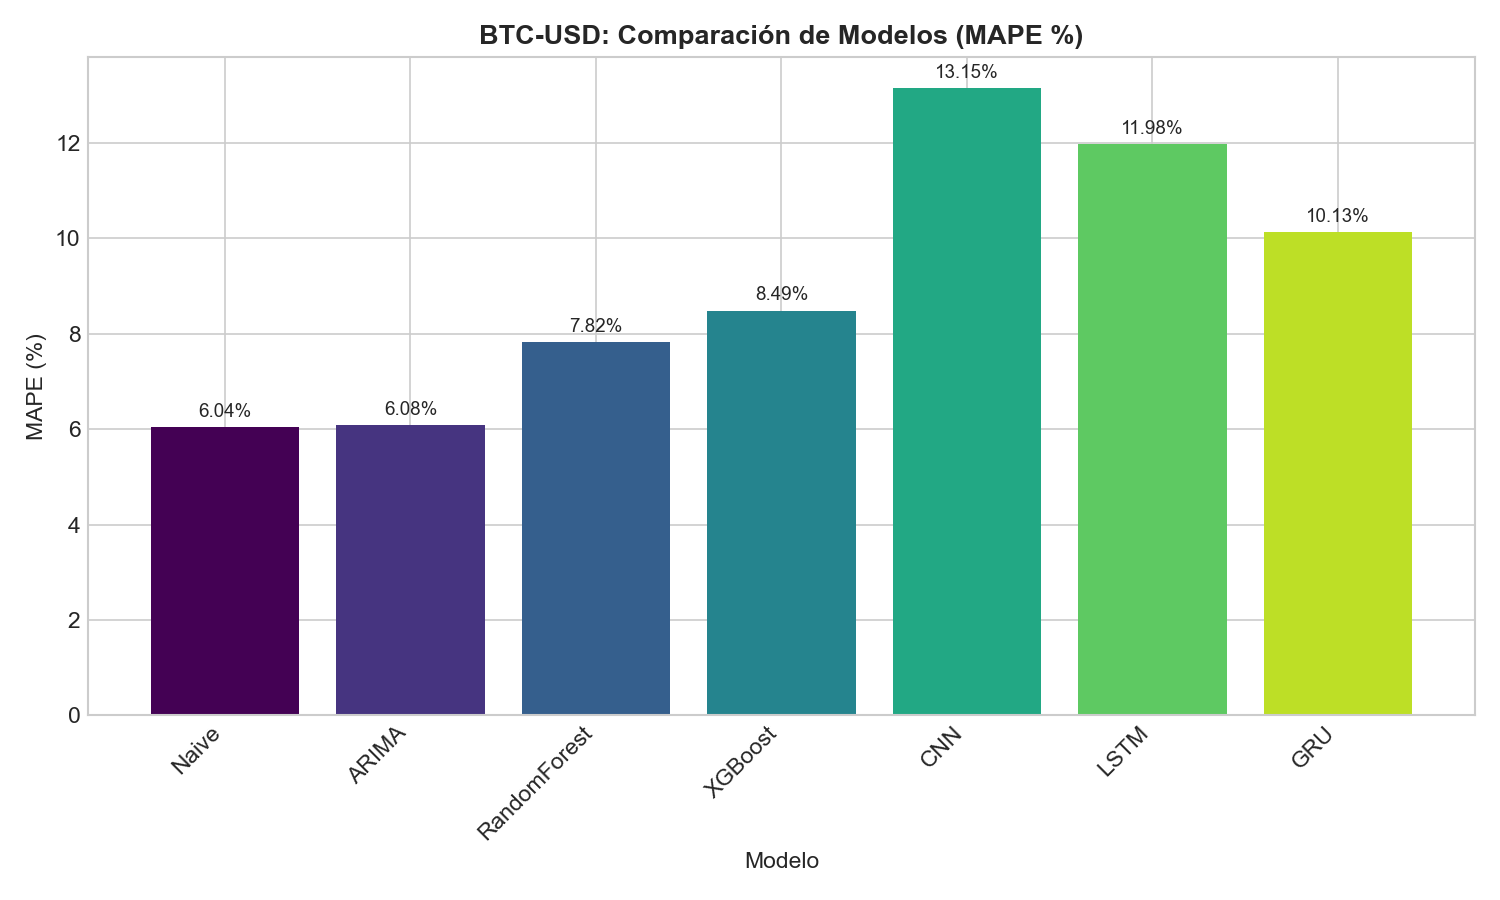
\includegraphics[width=0.95\textwidth]{Imagenes/model_comparison_BTC_USD_mape.png}
\caption{BTC-USD: Comparación de modelos (MAPE \%).}
\label{fig:model_btc_mape}
\end{figure}

\begin{figure}[H]
\centering
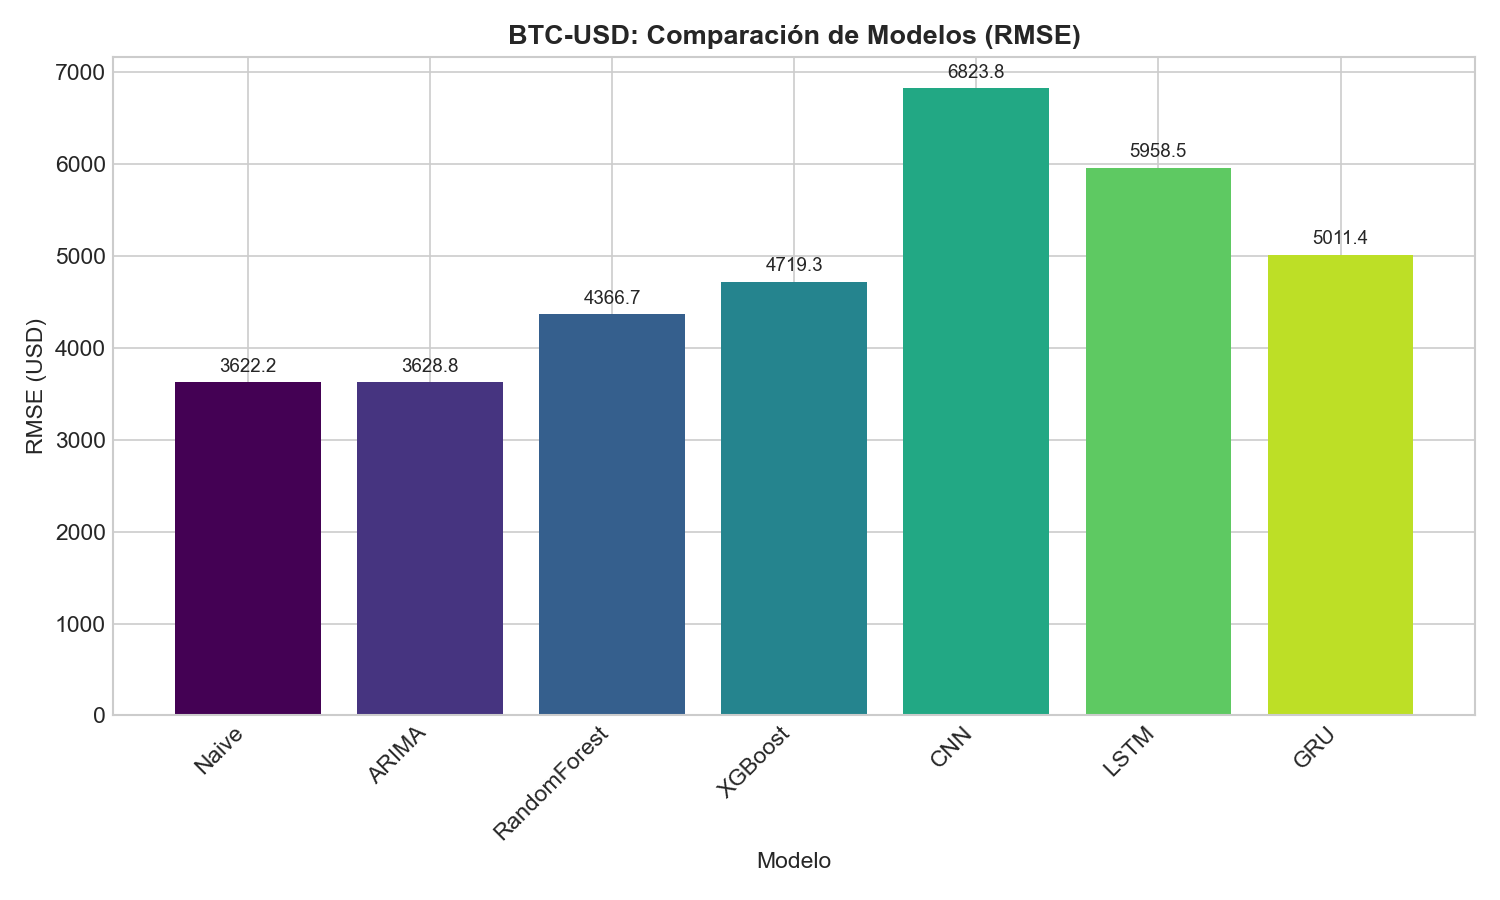
\includegraphics[width=0.95\textwidth]{Imagenes/model_comparison_BTC_USD_rmse.png}
\caption{BTC-USD: Comparación de modelos (RMSE en USD).}
\label{fig:model_btc_rmse}
\end{figure}

En Bitcoin, Naive obtiene el mejor MAPE y ARIMA le sigue de cerca. Los modelos de árboles no solo no mejoran, sino que empeoran de forma apreciable (XGBoost especialmente). Las redes profundas quedan aún más lejos: GRU es la que presenta menor error dentro de las arquitecturas DL, pero incluso esta se aleja de forma notable de los baselines.

La lectura práctica es que Bitcoin sigue siendo un activo difícil para los modelos predictivos. Su volatilidad es tan elevada que un baseline trivial como ``mañana valdrá lo mismo que hoy'' ya es difícil de mejorar. Si ni siquiera añadir indicadores técnicos y sentimiento basta para superar al Naive, es que la señal disponible no compensa el ruido.

\subsection{Tesla: ARIMA toma ventaja}

Las Figuras~\ref{fig:model_tsla_mape} y \ref{fig:model_tsla_rmse} muestran los resultados para Tesla.

\begin{figure}[H]
\centering
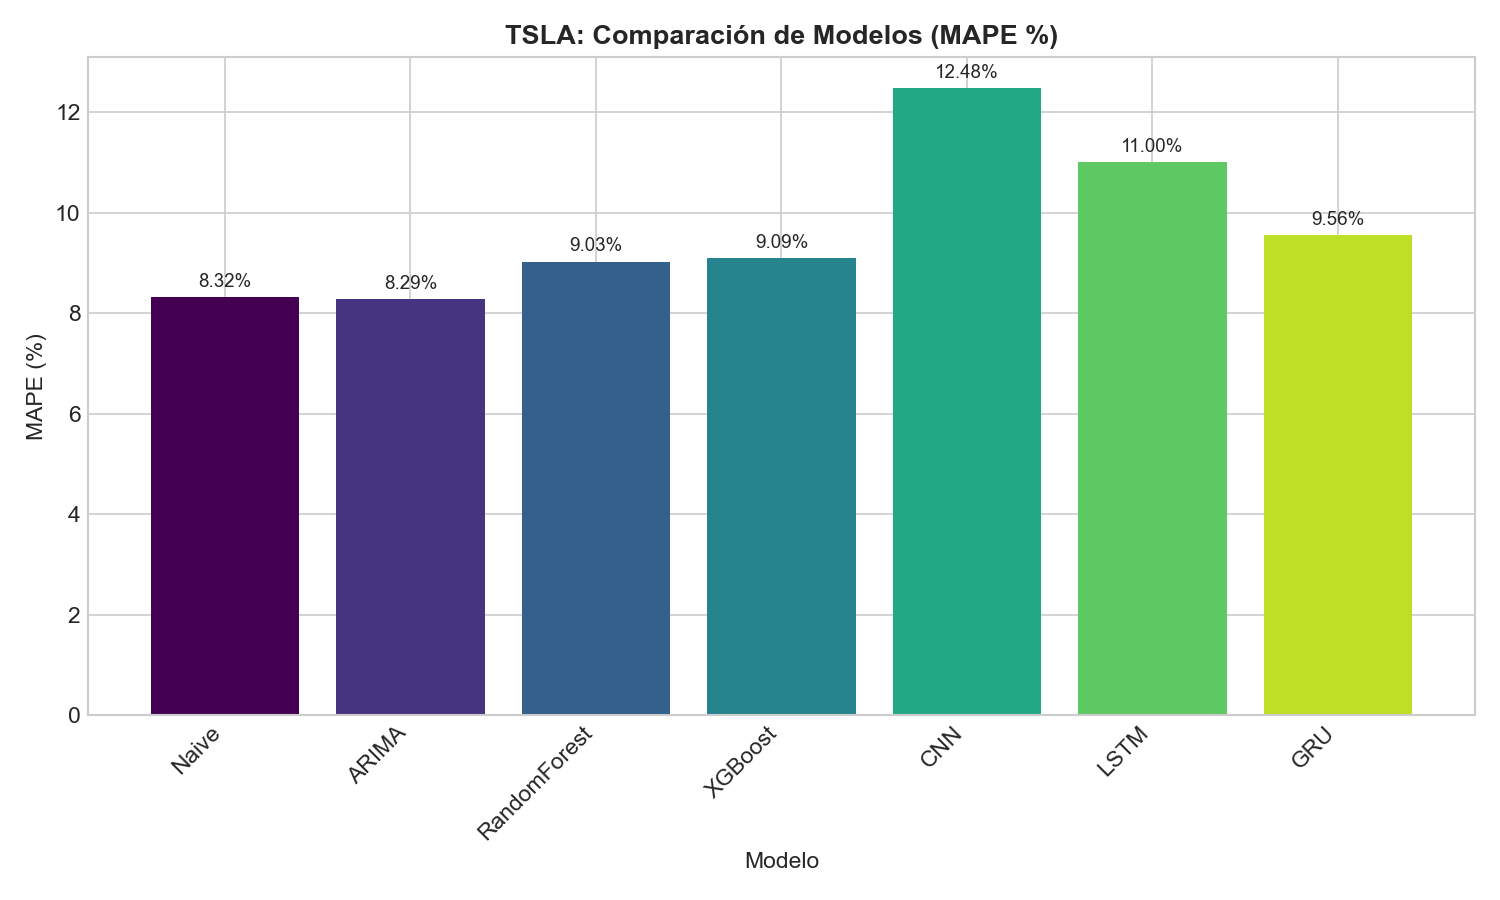
\includegraphics[width=0.95\textwidth]{Imagenes/model_comparison_TSLA_mape.png}
\caption{TSLA: Comparación de modelos (MAPE \%).}
\label{fig:model_tsla_mape}
\end{figure}

\begin{figure}[H]
\centering
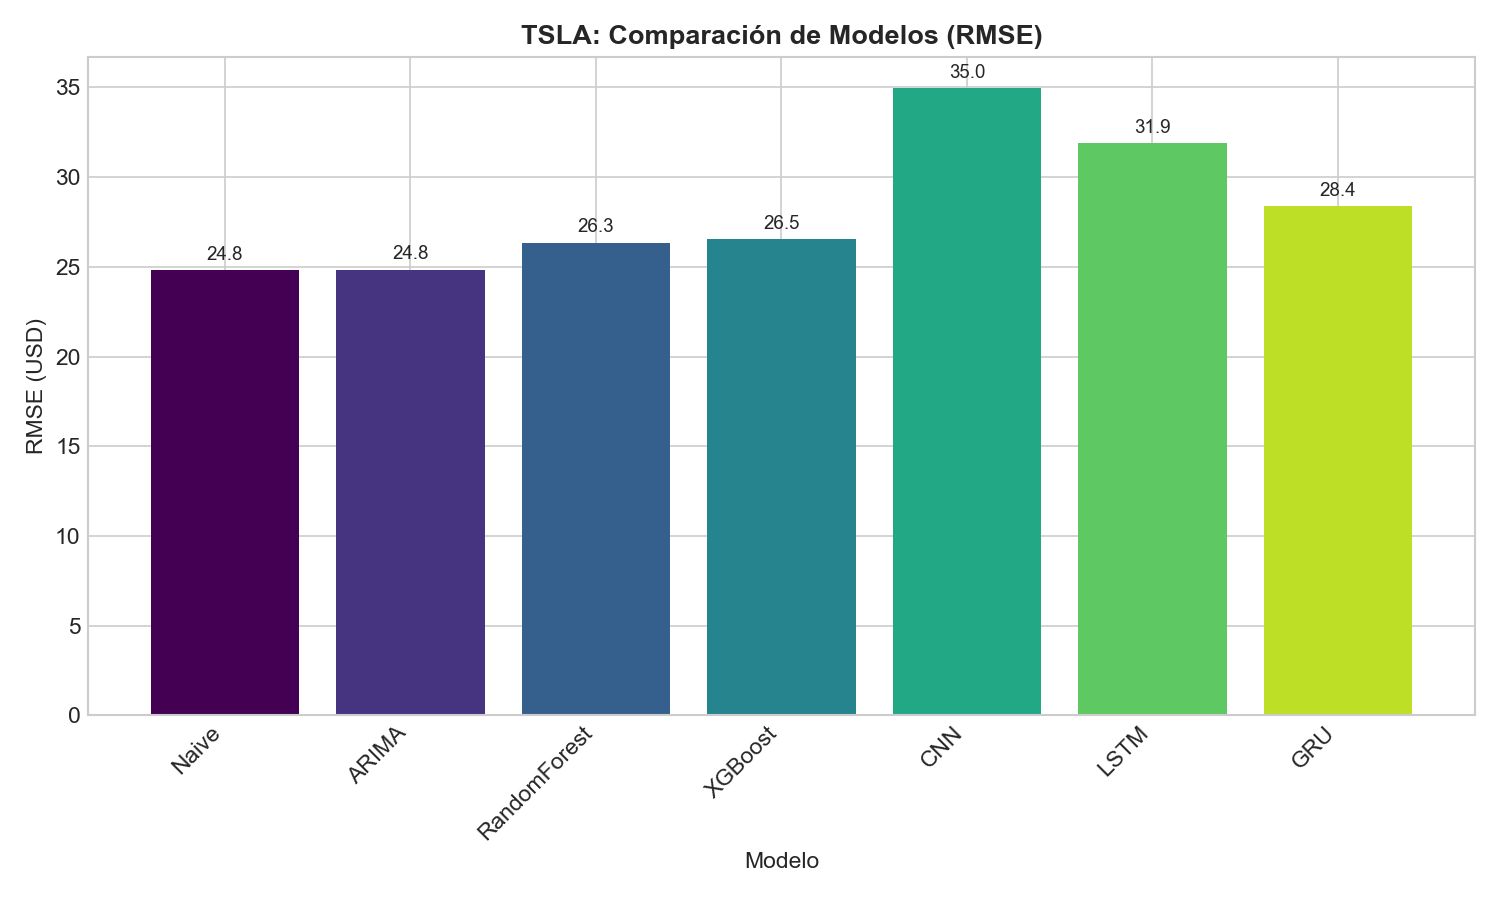
\includegraphics[width=0.95\textwidth]{Imagenes/model_comparison_TSLA_rmse.png}
\caption{TSLA: Comparación de modelos (RMSE en USD).}
\label{fig:model_tsla_rmse}
\end{figure}

En Tesla, ARIMA pasa a ser el mejor en MAPE y Naive queda prácticamente empatado. Los modelos de árboles no superan a los baselines y quedan por encima, aunque la diferencia es menor que en BTC-USD. Las redes profundas no resultan competitivas en esta configuración experimental: GRU es el modelo con menor error dentro de DL, pero aun así queda por encima de Naive/ARIMA, y CNN es la que más se degrada. Esto sugiere que, con series con cambios de régimen, aumentar la complejidad sin un tuning cuidadoso puede empeorar la generalización.

El rendimiento de Random Forest y XGBoost es razonable pero no aporta ventaja clara con retardos simples. Una ingeniería de características más rica (o modelos diseñados específicamente para forecasting tabular) podría mejorar su posición, pero en este trabajo se priorizó la comparativa entre familias de modelos sin optimización exhaustiva.

\subsection{Nvidia: ARIMA destaca}

Las Figuras~\ref{fig:model_nvda_mape} y \ref{fig:model_nvda_rmse} muestran los resultados para Nvidia.

\begin{figure}[H]
\centering
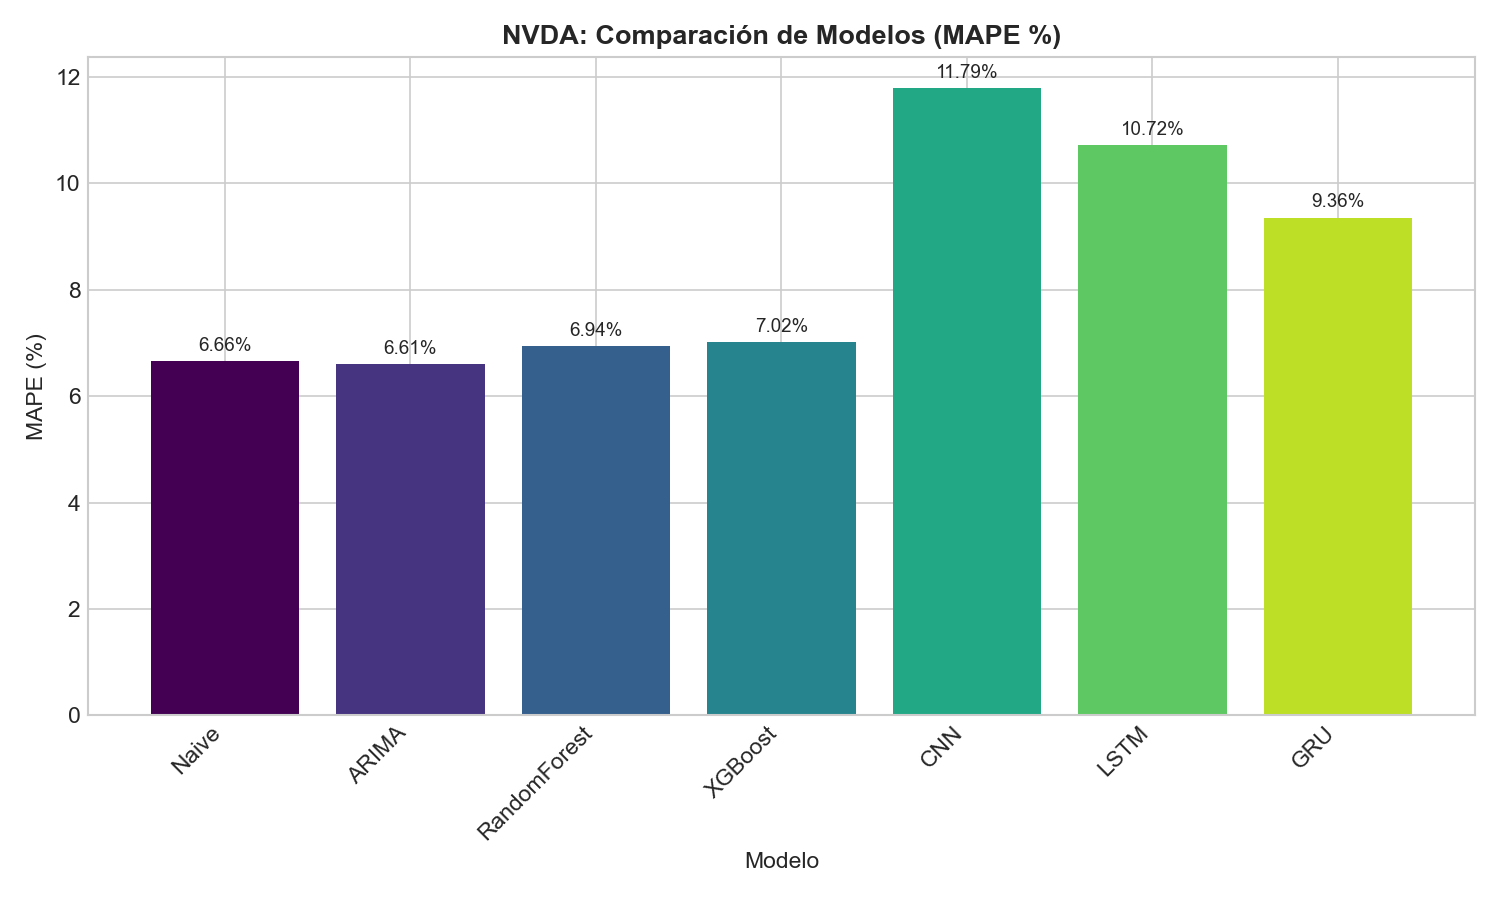
\includegraphics[width=0.95\textwidth]{Imagenes/model_comparison_NVDA_mape.png}
\caption{NVDA: Comparación de modelos (MAPE \%).}
\label{fig:model_nvda_mape}
\end{figure}

\begin{figure}[H]
\centering
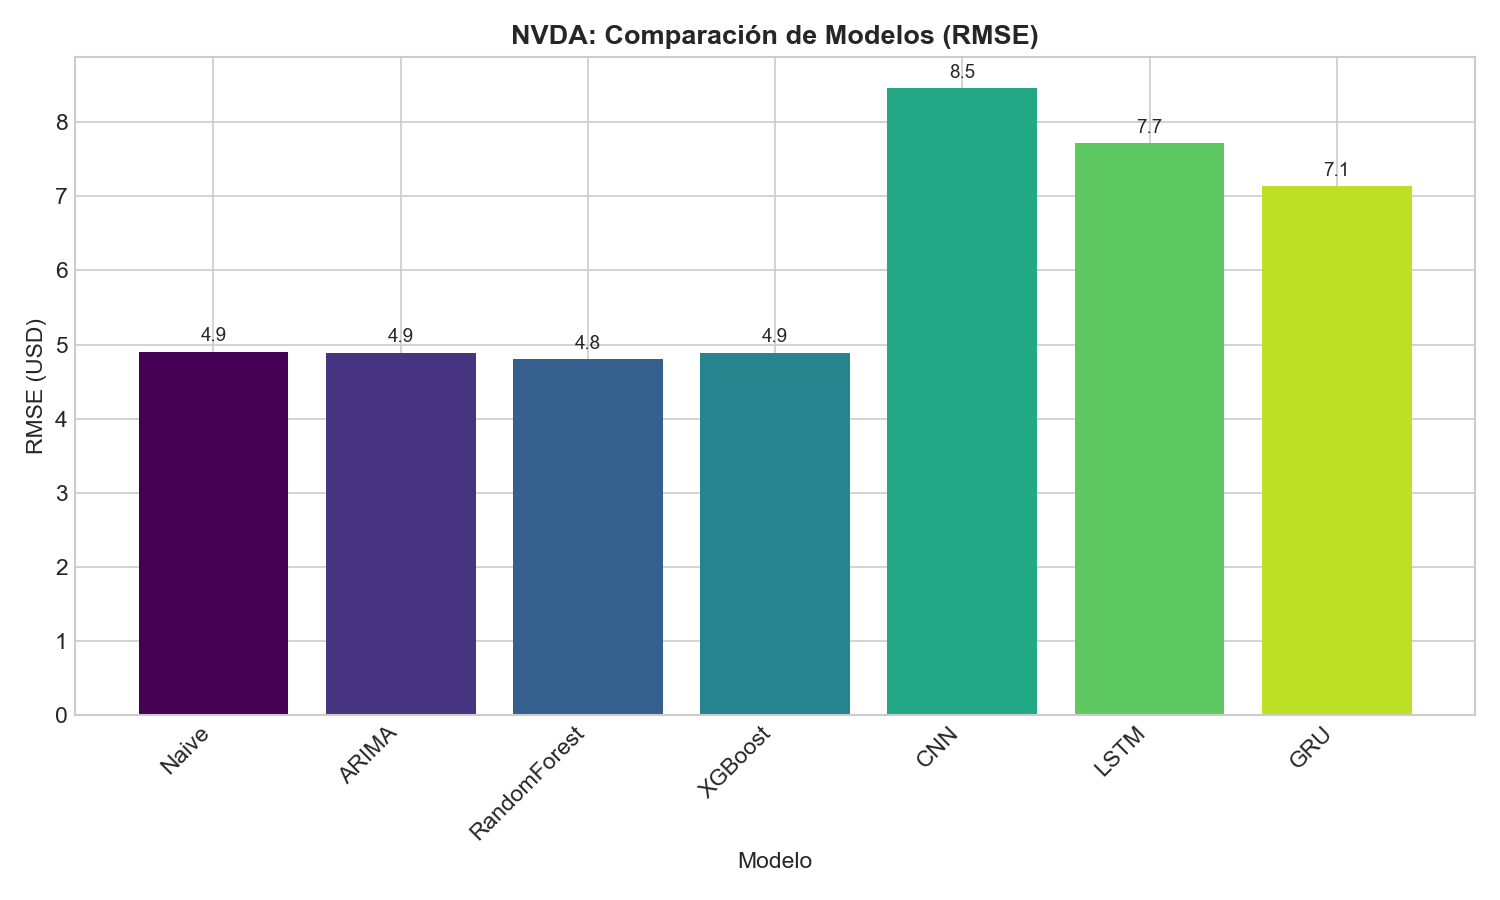
\includegraphics[width=0.95\textwidth]{Imagenes/model_comparison_NVDA_rmse.png}
\caption{NVDA: Comparación de modelos (RMSE en USD).}
\label{fig:model_nvda_rmse}
\end{figure}

En Nvidia, \textbf{ARIMA} marca el mejor MAPE, con Naive prácticamente empatado. Random Forest y XGBoost se quedan relativamente cerca pero no mejoran a los baselines. Las redes profundas vuelven a estar claramente por detrás (especialmente CNN y LSTM); GRU se aproxima más, pero no alcanza a ARIMA/Naive.

El hecho de que ARIMA y Naive estén tan próximos invita a no sobreinterpretar pequeñas diferencias: en un activo con cambios de régimen frecuentes, la estabilidad del rendimiento pesa casi tanto como la media.

\subsection{Visión de conjunto}

Para facilitar la comparación entre modelos y activos, se generaron varias visualizaciones de síntesis. La Figura~\ref{fig:cross_asset_heatmap} presenta un mapa de calor que resume el MAPE de cada modelo por activo. Los colores más fríos (azul) indican menor error y, por tanto, mejor rendimiento. Esta visualización permite identificar rápidamente qué combinaciones modelo-activo funcionan mejor y detectar patrones transversales.

\begin{figure}[H]
\centering
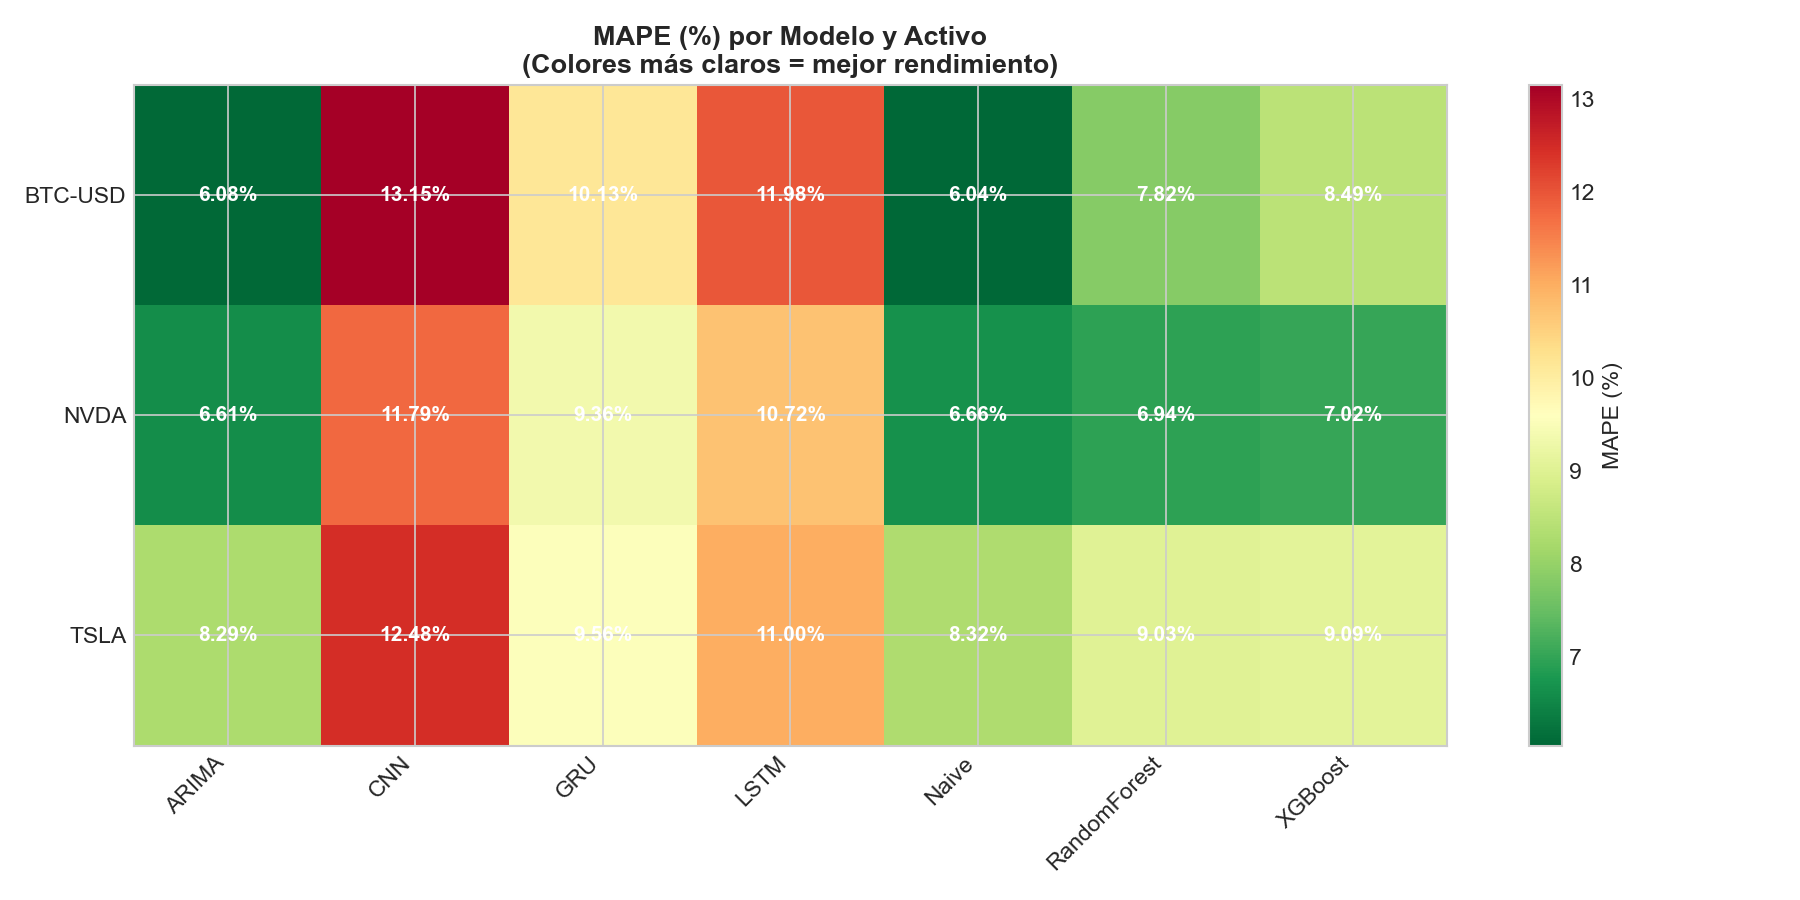
\includegraphics[width=0.95\textwidth]{Imagenes/cross_asset_heatmap.png}
\caption{Mapa de calor: MAPE (\%) por modelo y activo.}
\label{fig:cross_asset_heatmap}
\end{figure}

Complementando el mapa de calor, la Figura~\ref{fig:cross_asset_bar} presenta la misma información en formato de barras agrupadas, lo que facilita la comparación directa de la magnitud del error entre modelos dentro de cada activo. Este formato es especialmente útil para identificar cuánto mejor o peor es cada modelo respecto a los demás en términos absolutos.

\begin{figure}[H]
\centering
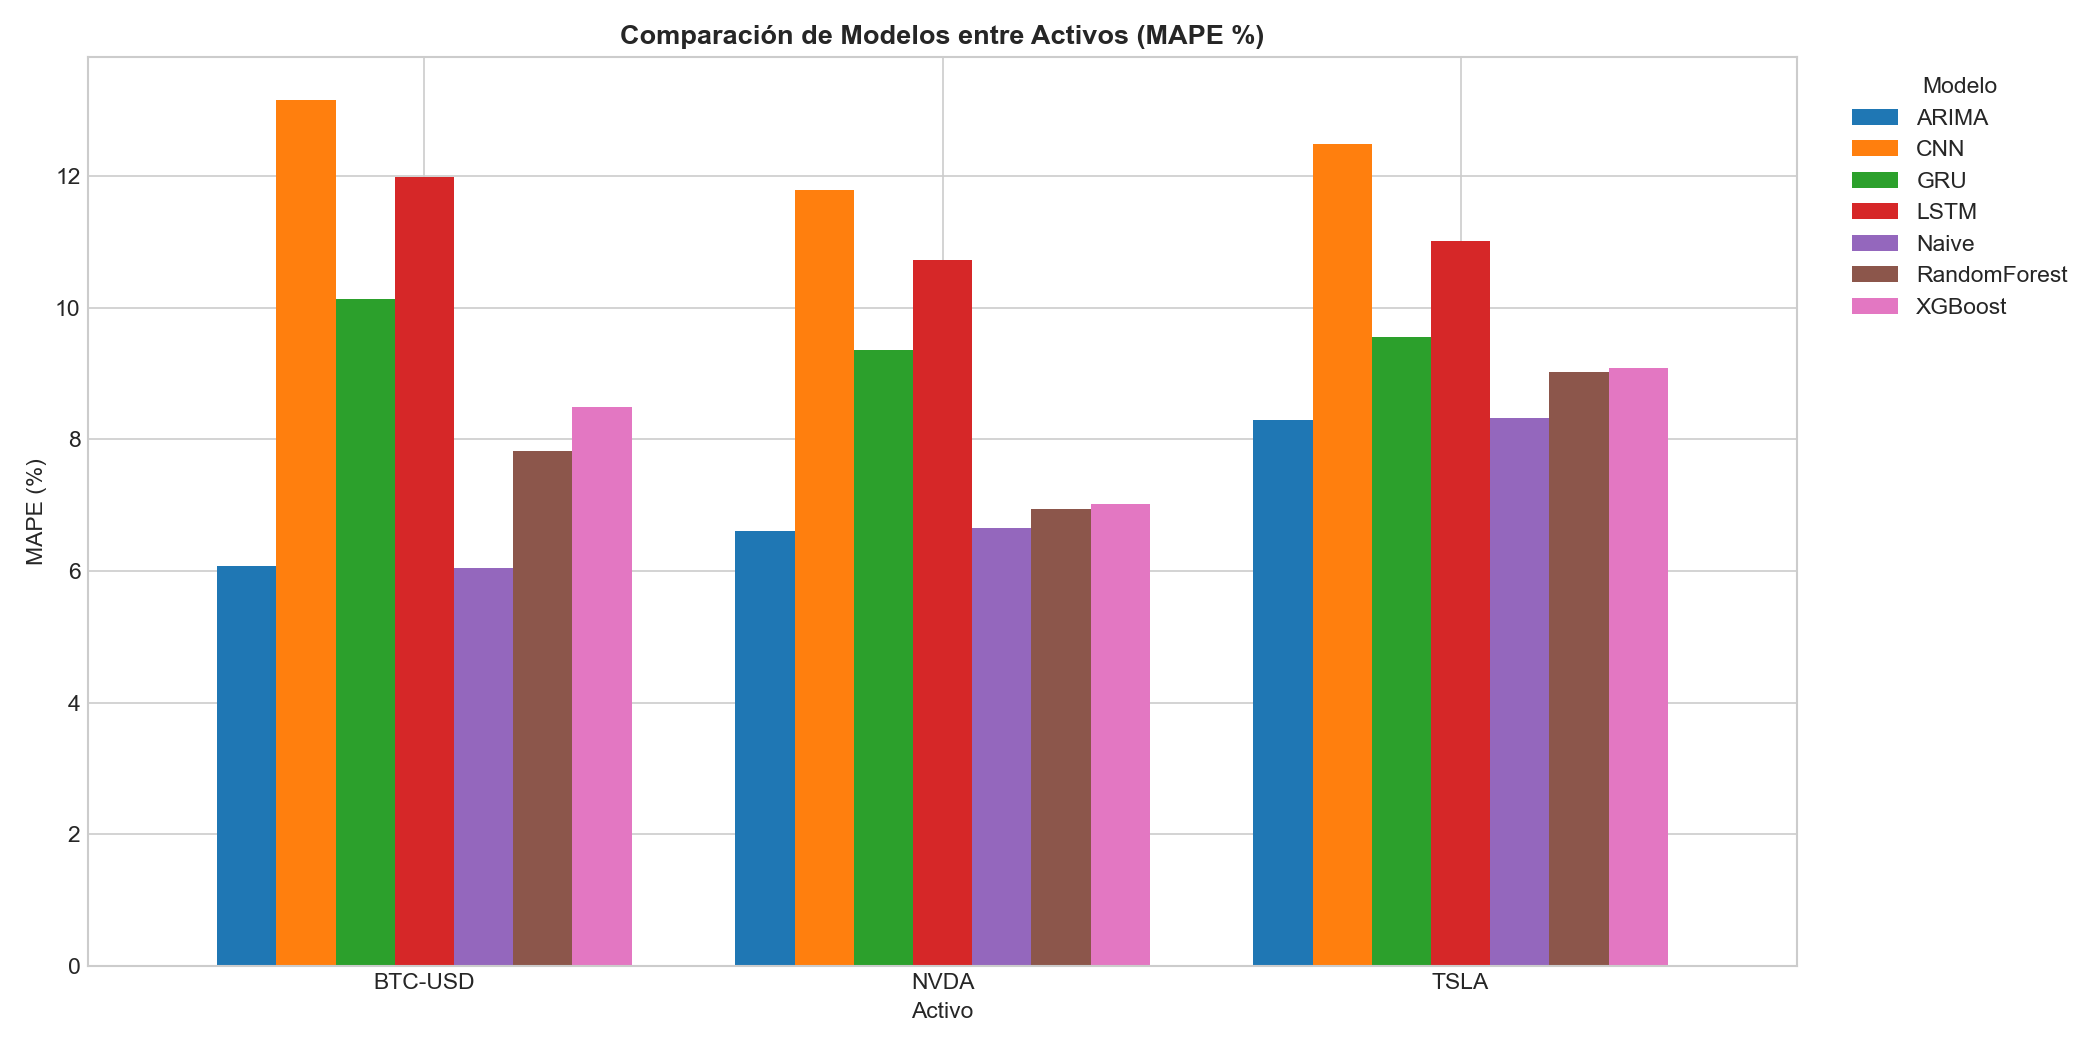
\includegraphics[width=0.95\textwidth]{Imagenes/cross_asset_grouped_bar.png}
\caption{Comparación agrupada de modelos entre activos.}
\label{fig:cross_asset_bar}
\end{figure}

Además de comparar medias, resulta fundamental analizar la dispersión del error. La Figura~\ref{fig:error_dist_all} muestra la distribución del MAPE mediante diagramas de caja (boxplots). Esta visualización permite identificar no solo qué modelo tiene menor error medio, sino también cuál presenta mayor estabilidad en sus predicciones. Un modelo con baja mediana pero alta dispersión (caja ancha) puede ser menos fiable en la práctica que otro con error algo mayor pero más consistente.

\begin{figure}[H]
\centering
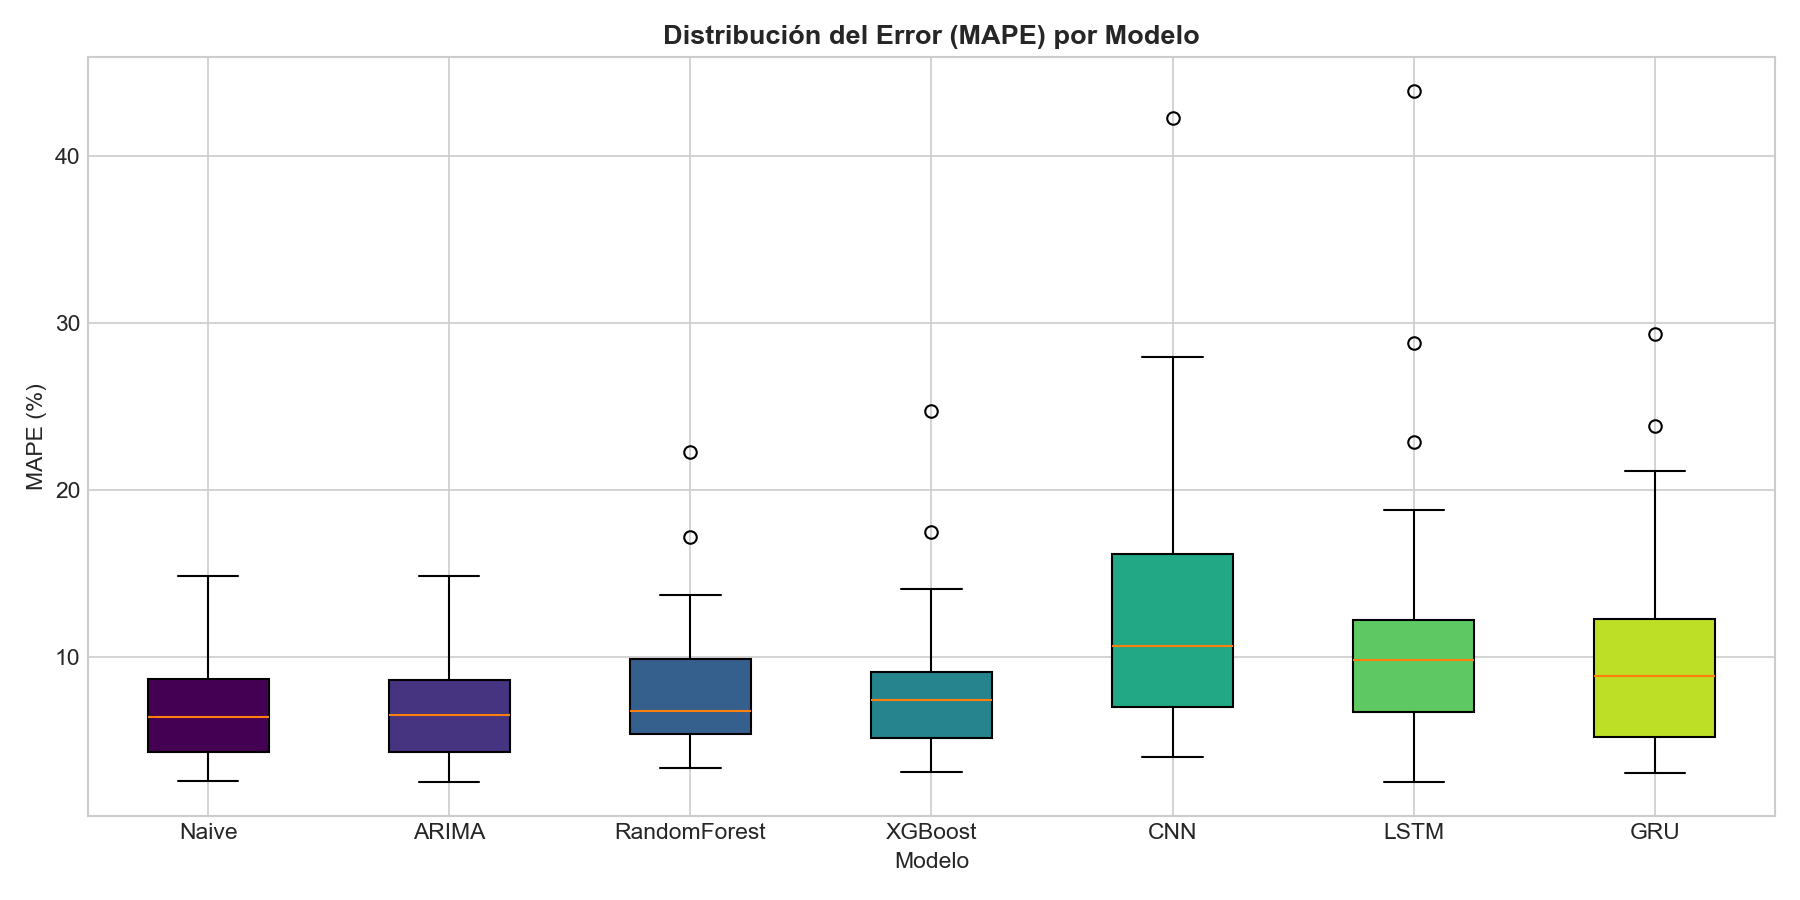
\includegraphics[width=0.95\textwidth]{Imagenes/error_distribution_boxplot.png}
\caption{Distribución del error MAPE por modelo.}
\label{fig:error_dist_all}
\end{figure}

Además de la media, resulta útil ver la dispersión por fold. La Figura~\ref{fig:mape_dispersion} resume el MAPE medio y su variabilidad, que ayuda a distinguir modelos estables de modelos con rendimiento errático.

\begin{figure}[H]
\centering
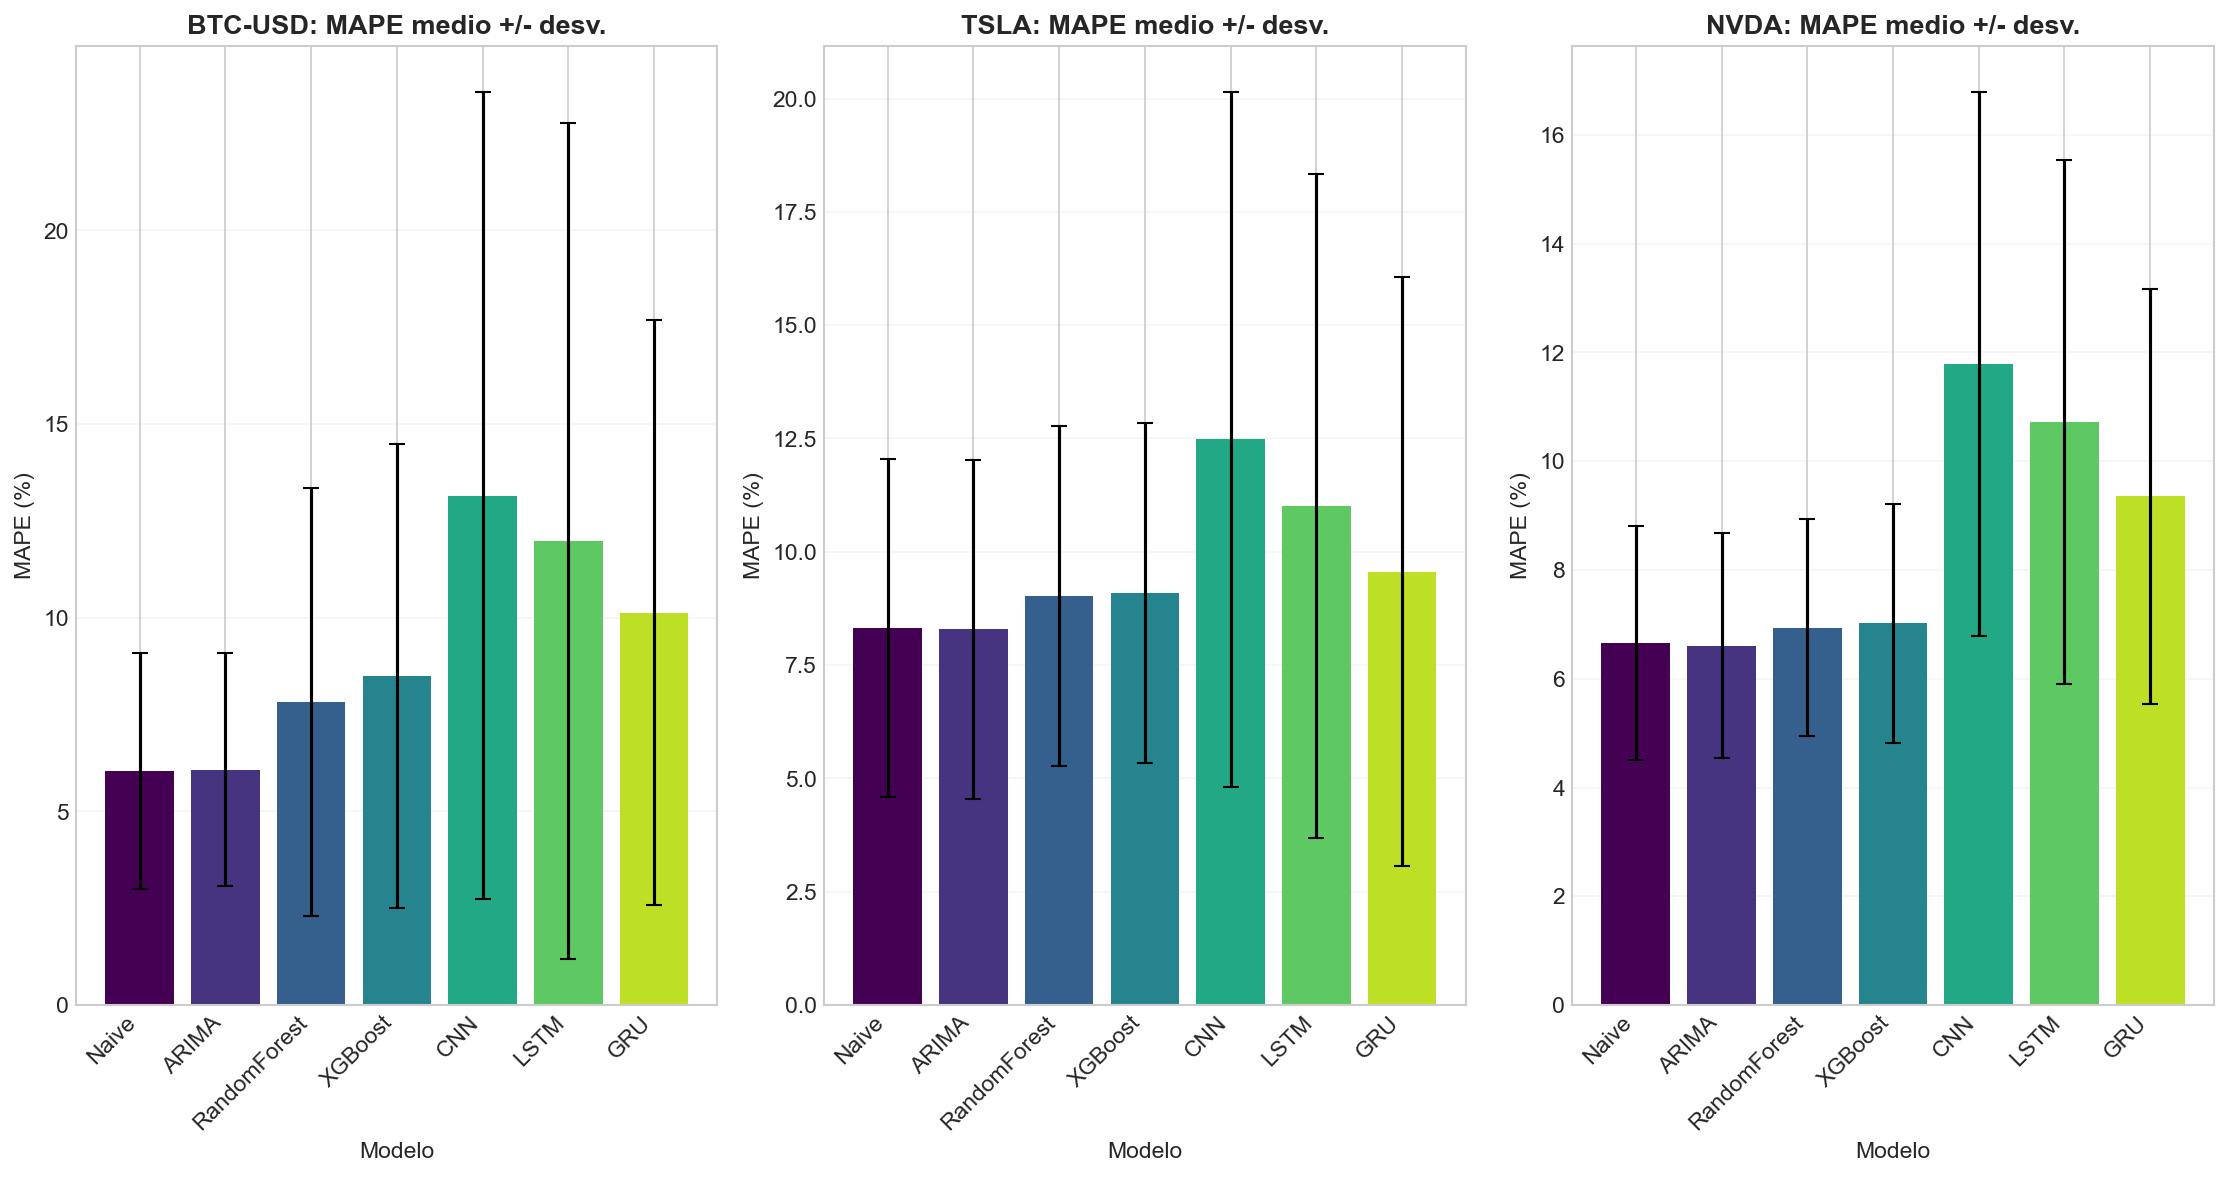
\includegraphics[width=0.95\textwidth]{Imagenes/model_comparison_mape_dispersion.png}
\caption{MAPE medio y dispersión por fold en cada activo.}
\label{fig:mape_dispersion}
\end{figure}

Estas tres vistas (heatmap, barras y boxplot) reflejan el mismo patrón desde perspectivas distintas: los baselines lideran de forma consistente y la dispersión de errores es relevante al comparar modelos no-baseline. En la práctica, un modelo con mejor media pero muy inestable puede ser peor elección que otro ligeramente peor pero más consistente.

Implicación práctica: si se necesita un modelo ``por defecto'' para repetir este experimento, \textbf{ARIMA} y \textbf{Naive} son referencias muy fuertes (Naive lidera BTC-USD y ARIMA lidera TSLA/NVDA). En este trabajo, ni los modelos de árboles ni los modelos DL justifican su complejidad frente a esos baselines en términos de MAPE.

%% ============================================================
%% EXPERIMENTO B: IMPACTO DEL HORIZONTE
%% ============================================================

\section{Impacto del horizonte de predicción (BTC-USD)}

Era previsible que la predicción resultara más difícil a mayor horizonte. La incertidumbre se acumula y la probabilidad de que ocurra algo inesperado crece con los días. Este experimento cuantifica dicha expectativa.

\subsection{Los números}

La Tabla~\ref{tab:experiment_b} compara los horizontes de 1, 7 y 30 días para Bitcoin.

\begin{table}[H]
\centering
\caption{MAPE (\%) por horizonte para BTC-USD}
\label{tab:experiment_b}
\begin{tabular}{l|ccc}
\hline
\textbf{Modelo} & \textbf{1 dia} & \textbf{7 dias} & \textbf{30 dias} \\
\hline
CNN & 7.71 & 13.15 & 20.93 \\
GRU & \textbf{5.58} & \textbf{10.13} & \textbf{20.11} \\
LSTM & 8.11 & 11.98 & 26.16 \\
\hline
\end{tabular}
\end{table}

Como era de esperar, todos los modelos empeoran a medida que aumenta el horizonte. En BTC-USD el salto es sustancial: el MAPE pasa de un orden del 5--8\% a 1 día a valores cercanos al 20\% a 30 días. Dentro de los modelos DL, GRU es el más consistente y mantiene el menor MAPE en los tres horizontes; LSTM y CNN degradan más, especialmente a 30 días. La Figura~\ref{fig:horizon_all_models} ilustra esta degradación.

\begin{figure}[H]
\centering
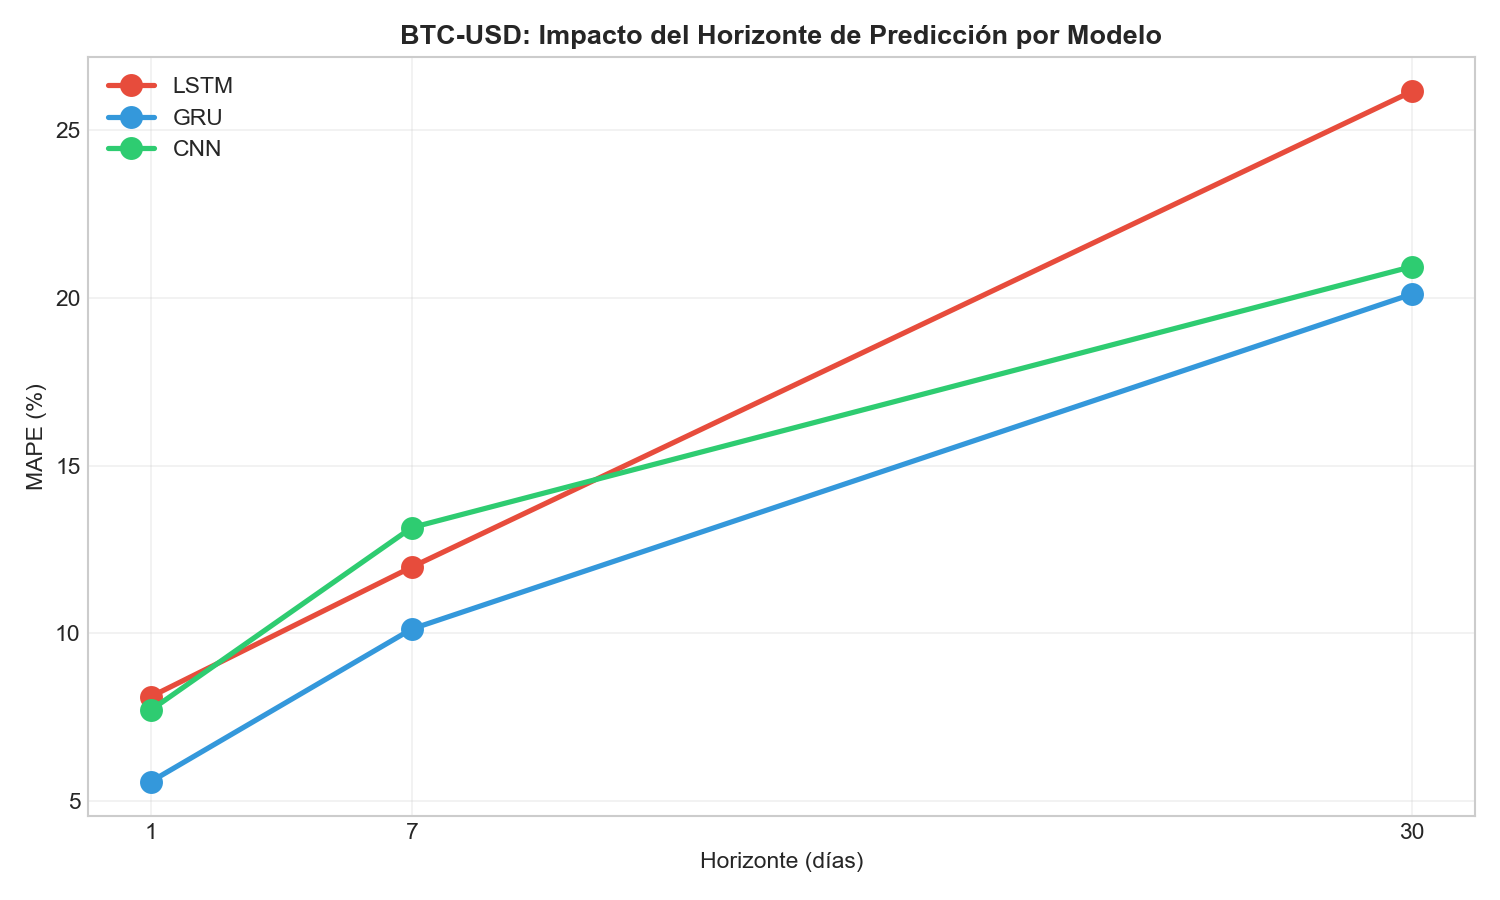
\includegraphics[width=0.90\textwidth]{Imagenes/horizon_impact_all_models.png}
\caption{Impacto del horizonte por modelo.}
\label{fig:horizon_all_models}
\end{figure}

Para analizar en detalle cómo se comporta cada arquitectura a medida que aumenta el horizonte, las Figuras~\ref{fig:horizon_lstm}, \ref{fig:horizon_gru} y \ref{fig:horizon_cnn} desglosan las métricas (RMSE, MAE y MAPE) por modelo. Estas visualizaciones permiten identificar no solo cuál modelo escala mejor, sino también detectar comportamientos anómalos ---por ejemplo, que un modelo degrade más rápido de lo esperado o que mantenga su rendimiento de forma atípica---.

\begin{figure}[H]
\centering
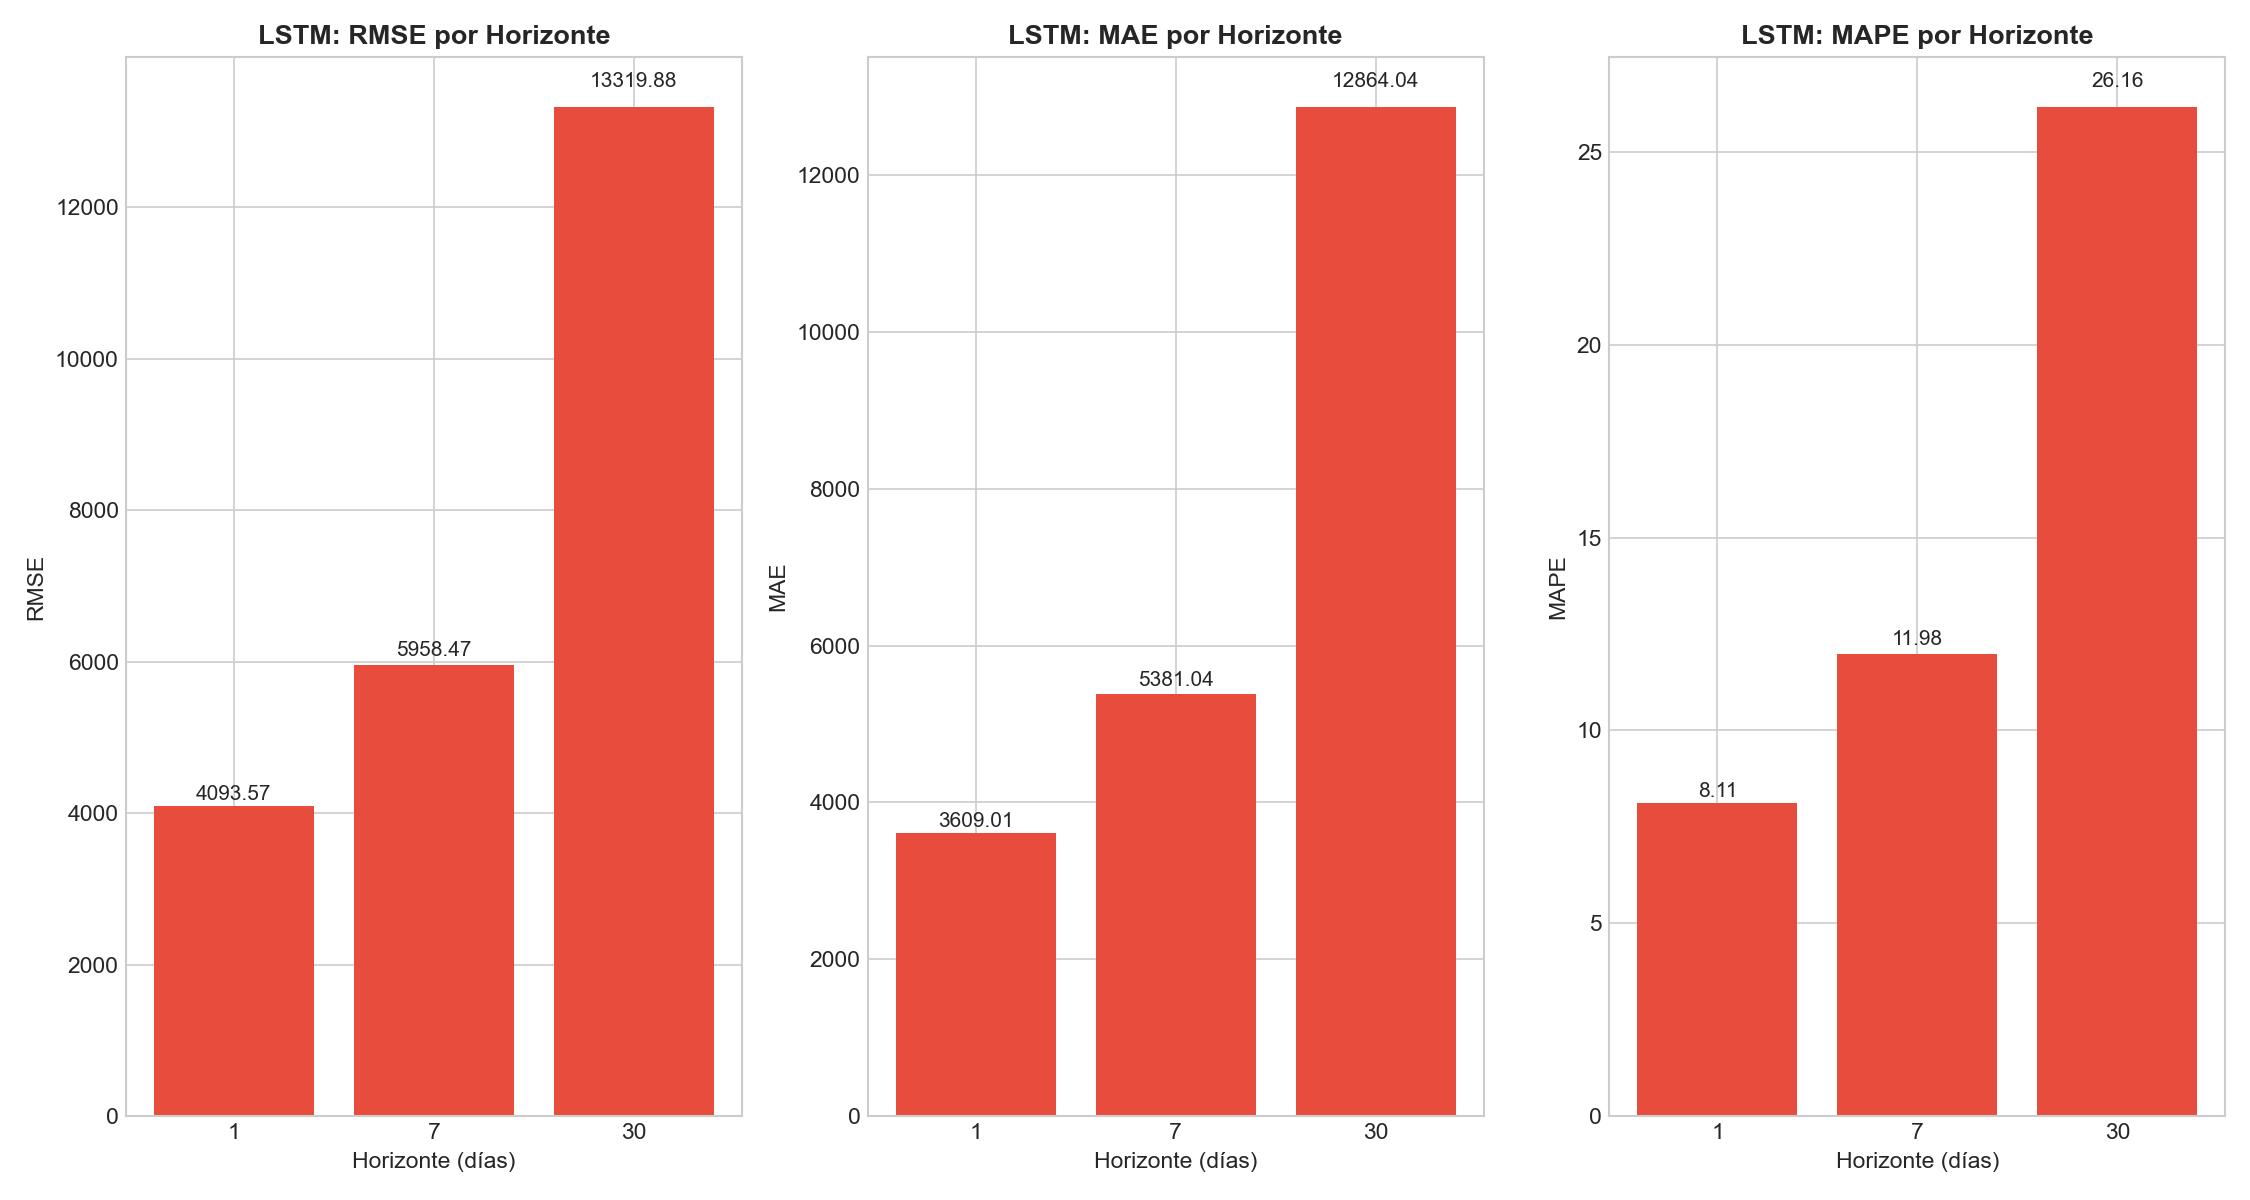
\includegraphics[width=0.95\textwidth]{Imagenes/horizon_impact_lstm_metrics.png}
\caption{LSTM: Métricas por horizonte. El error aumenta de forma marcada a medida que se alarga el horizonte, especialmente a 30 días.}
\label{fig:horizon_lstm}
\end{figure}

\begin{figure}[H]
\centering
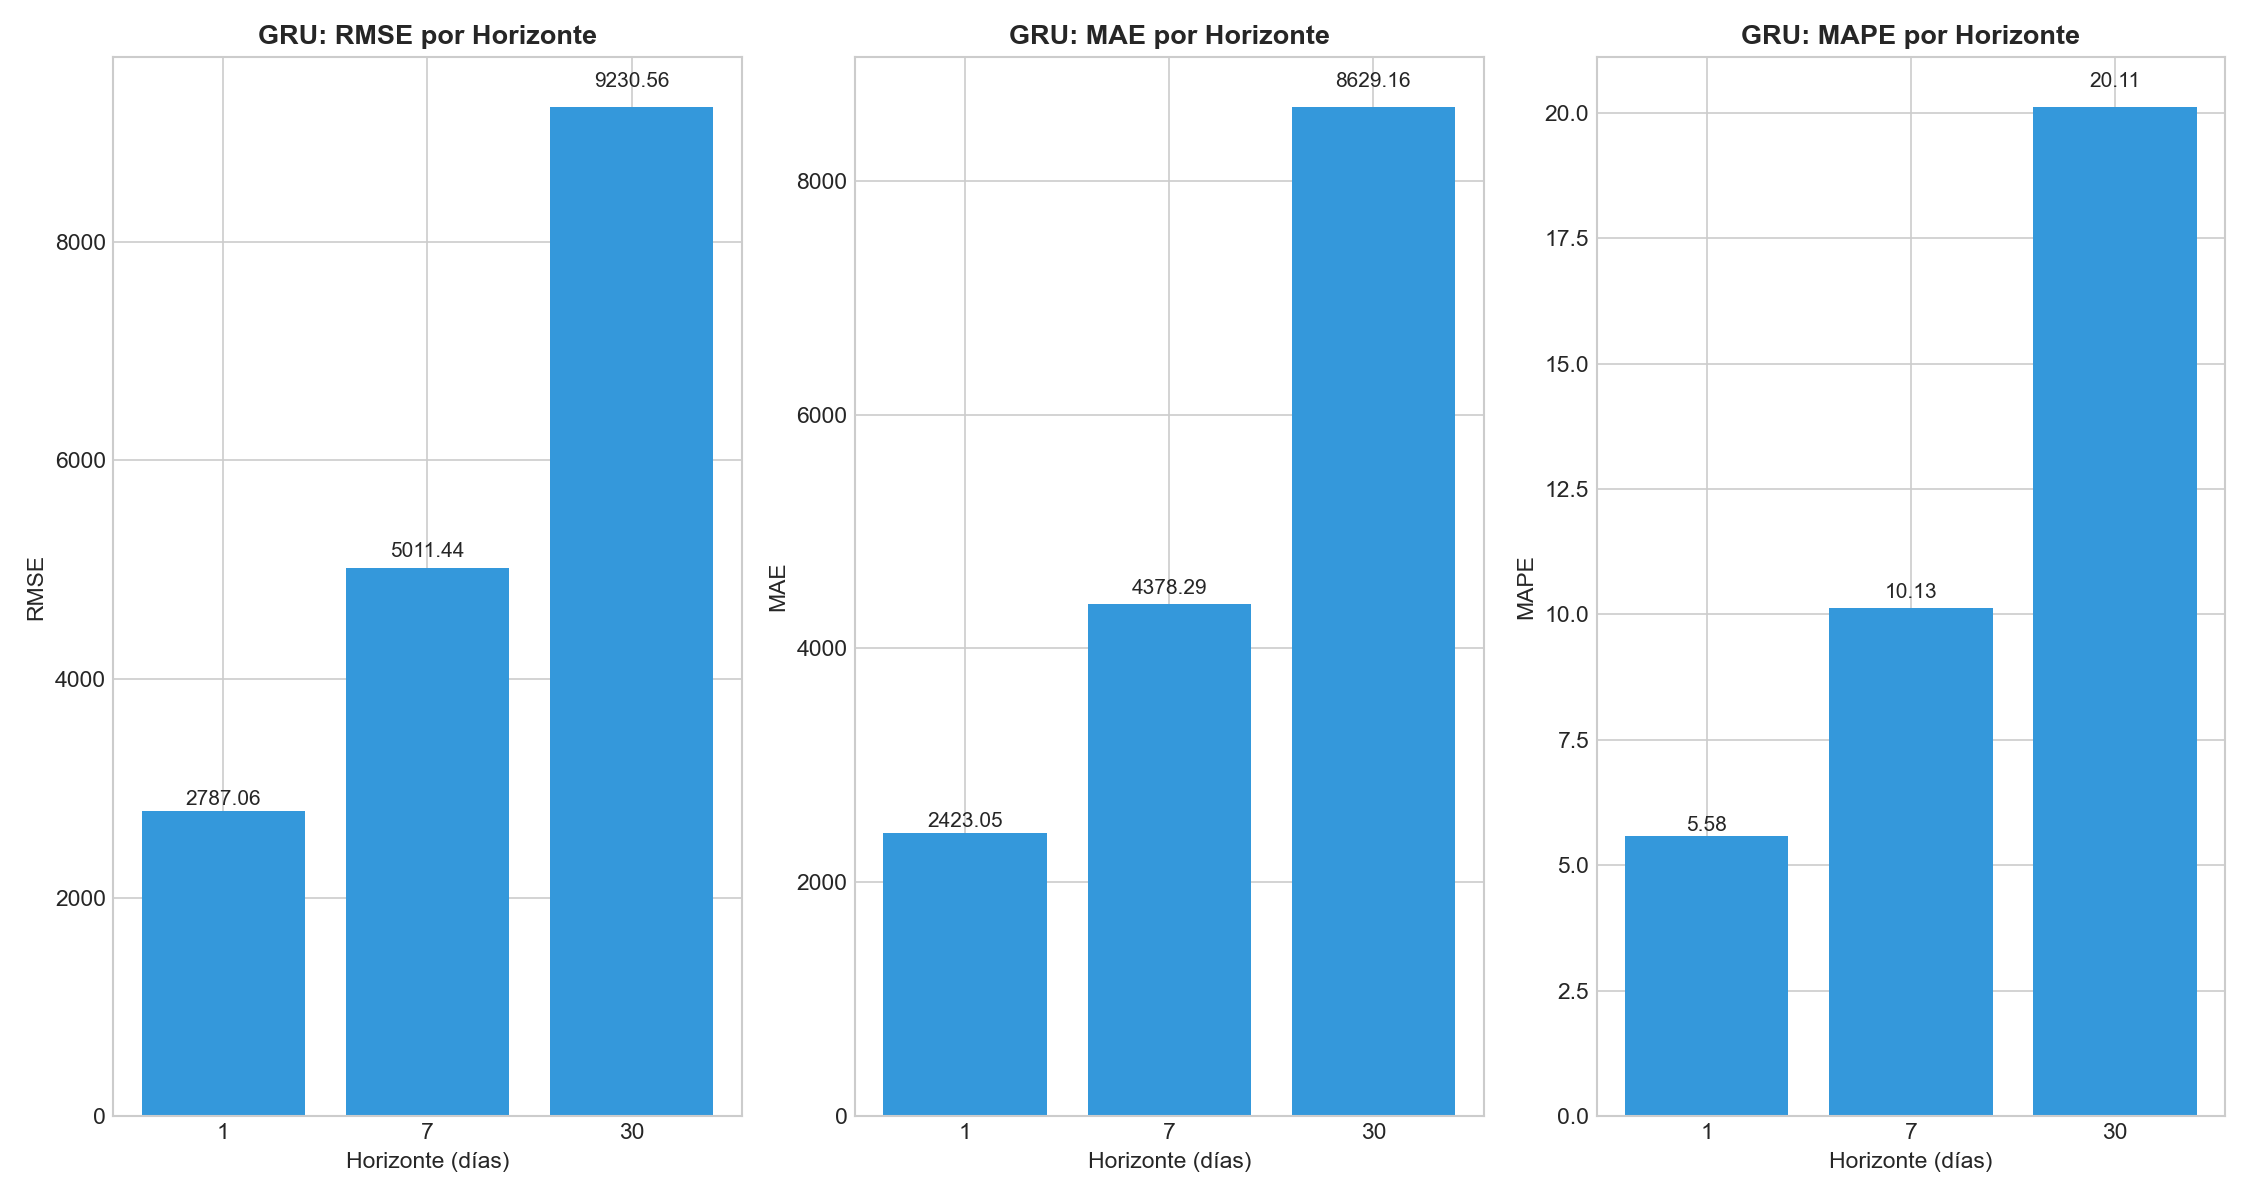
\includegraphics[width=0.95\textwidth]{Imagenes/horizon_impact_gru_metrics.png}
\caption{GRU: Métricas por horizonte. GRU muestra el comportamiento más estable de las tres arquitecturas, con una degradación más suave y valores consistentemente inferiores a LSTM y CNN en todos los horizontes.}
\label{fig:horizon_gru}
\end{figure}

\begin{figure}[H]
\centering
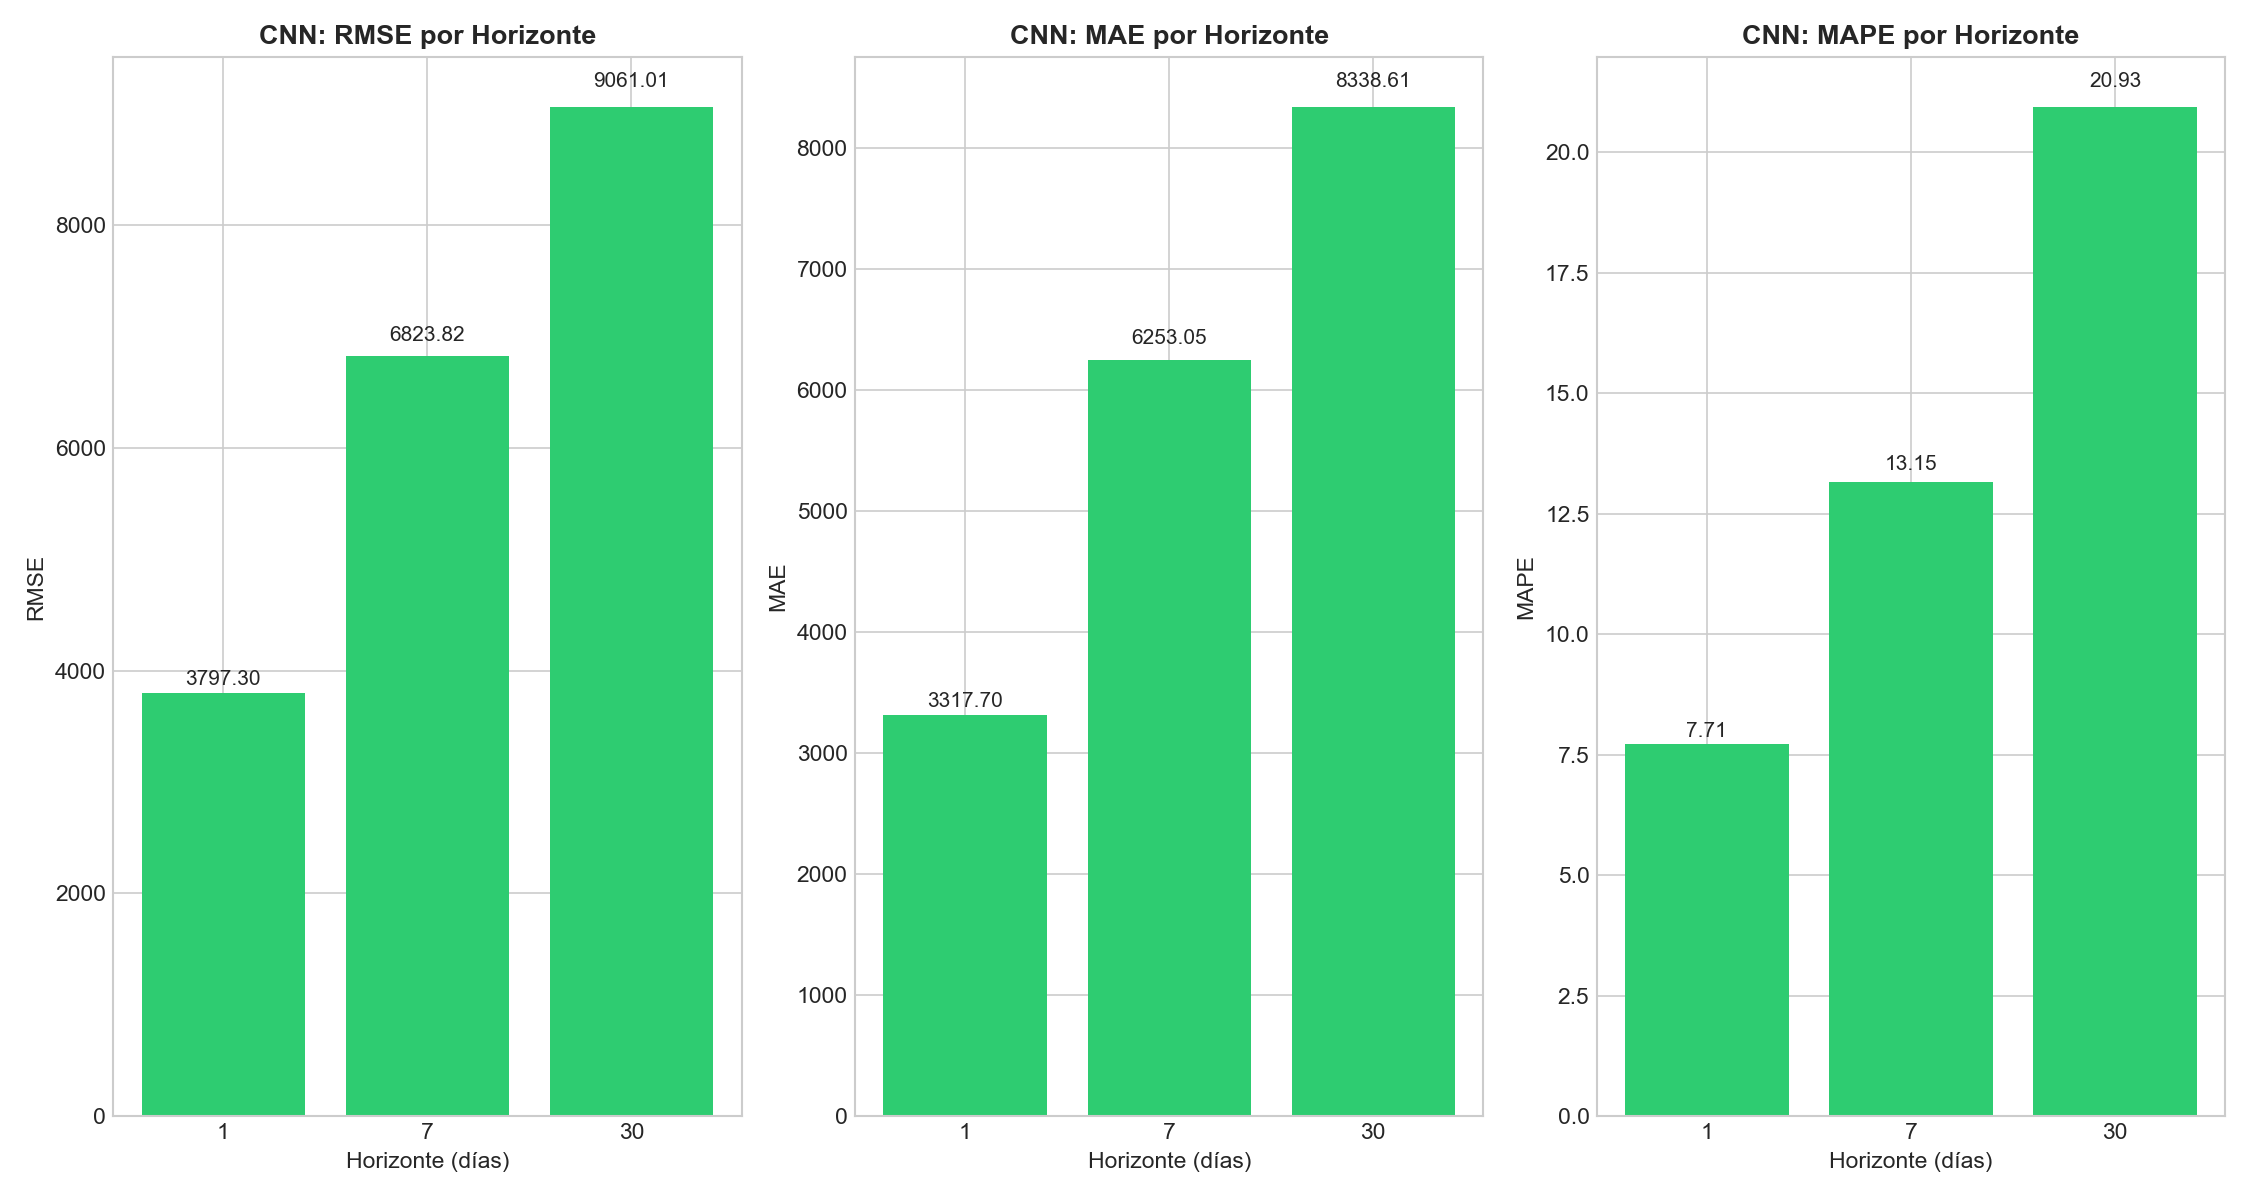
\includegraphics[width=0.95\textwidth]{Imagenes/horizon_impact_cnn_metrics.png}
\caption{CNN: Métricas por horizonte. CNN es la arquitectura que peor escala con el horizonte: aunque a 1 día se mueve en rangos similares, a 30 días el error aumenta de forma más pronunciada, evidenciando su limitación para capturar dependencias de largo plazo.}
\label{fig:horizon_cnn}
\end{figure}

La lección es clara dentro de la familia DL: GRU es el más robusto en todos los horizontes, aunque a 30 días los errores ya son altos. CNN, por el contrario, es la arquitectura que más sufre cuando el horizonte se alarga, lo que sugiere que su mecanismo de convolución local no captura adecuadamente las dependencias temporales extendidas necesarias para predicciones a largo plazo.

Desde un punto de vista operativo, esto pone un límite práctico: cuanto más lejos se intenta predecir, mayor es el coste en error. Si el objetivo es apoyar decisiones a corto plazo, el horizonte de 7 días parece un compromiso razonable; para 30 días, la señal se diluye demasiado.

Implicación práctica: si la predicción va a usarse en un contexto real, resulta más conveniente optimizar horizontes cortos y consistentes que perseguir horizontes largos con errores elevados.

%% ============================================================
%% EXPERIMENTO C: ABLACIÓN DE SENTIMIENTO
%% ============================================================

\section{Ablación de sentimiento (con vs sin)}

Este es el experimento central del trabajo. Se ejecutaron los modelos con y sin sentimiento para comprobar si contribuye de forma significativa a la predicción. El resultado principal es que el efecto existe, pero es \textbf{pequeño, y depende mucho del activo y del modelo}.

\subsection{Los números clave}

La Tabla~\ref{tab:experiment_c_full} muestra los resultados completos para todos los modelos de deep learning.

\begin{table}[H]
\centering
\caption{MAPE (\%) por modelo y activo, con y sin sentimiento}
\label{tab:experiment_c_full}
\begin{tabular}{l|l|cc|c}
\hline
\textbf{Activo} & \textbf{Modelo} & \textbf{Con Sent.} & \textbf{Sin Sent.} & \textbf{Ayuda?} \\
\hline
BTC-USD & CNN & 13.15 & 10.51 & \textcolor{red}{No (-25.1\%)} \\
BTC-USD & GRU & 10.13 & 9.16 & \textcolor{red}{No (-10.6\%)} \\
BTC-USD & LSTM & 11.98 & 10.94 & \textcolor{red}{No (-9.5\%)} \\
NVDA & CNN & 11.79 & 10.71 & \textcolor{red}{No (-10.1\%)} \\
NVDA & GRU & 9.36 & 8.95 & \textcolor{red}{No (-4.6\%)} \\
NVDA & LSTM & 10.72 & 10.96 & \textcolor{green!60!black}{Si (2.2\%)} \\
TSLA & CNN & 12.48 & 12.95 & \textcolor{green!60!black}{Si (3.6\%)} \\
TSLA & GRU & 9.56 & 9.82 & \textcolor{green!60!black}{Si (2.7\%)} \\
TSLA & LSTM & 11.00 & 11.32 & \textcolor{green!60!black}{Si (2.8\%)} \\
\hline
\end{tabular}
\end{table}

Los resultados muestran un patrón heterogéneo. El sentimiento \textbf{puede ayudar o perjudicar} según el activo:

\textbf{En Bitcoin, el sentimiento perjudica en los tres modelos.} El deterioro es especialmente marcado en CNN.

\textbf{En Tesla, el sentimiento mejora en los tres modelos.} La mejora existe, pero es moderada (del orden de unos pocos puntos porcentuales).

\textbf{En Nvidia, el efecto es mixto.} LSTM mejora ligeramente, mientras que CNN y GRU empeoran.

Estas diferencias pueden interpretarse como consecuencia de la naturaleza agregada de la señal de sentimiento y de la forma en que cada arquitectura integra variables externas. Bajo este protocolo, no se observa un patrón universal.

Estos resultados deben leerse en clave relativa. El test total es de 360 días, lo que mejora la estabilidad, pero un cambio de periodo puede mover bastante los porcentajes. Son resultados indicativos, no concluyentes; se discute de nuevo en la sección de limitaciones del capítulo final. La columna con sentimiento coincide con el experimento A; la comparación relevante es el salto frente a la columna sin sentimiento en cada modelo.

El porcentaje de mejora se calcula como $(\text{MAPE}_{\text{sin}} - \text{MAPE}_{\text{con}}) / \text{MAPE}_{\text{sin}}$. Valores positivos implican reducción del error al incluir sentimiento; valores negativos, empeoramiento. Las Figuras~\ref{fig:ablation_btc}--\ref{fig:ablation_nvda} muestran la ablación por activo, y la Figura~\ref{fig:ablation_heatmap} sintetiza los porcentajes de mejora en un mapa de calor.

\begin{figure}[H]
\centering
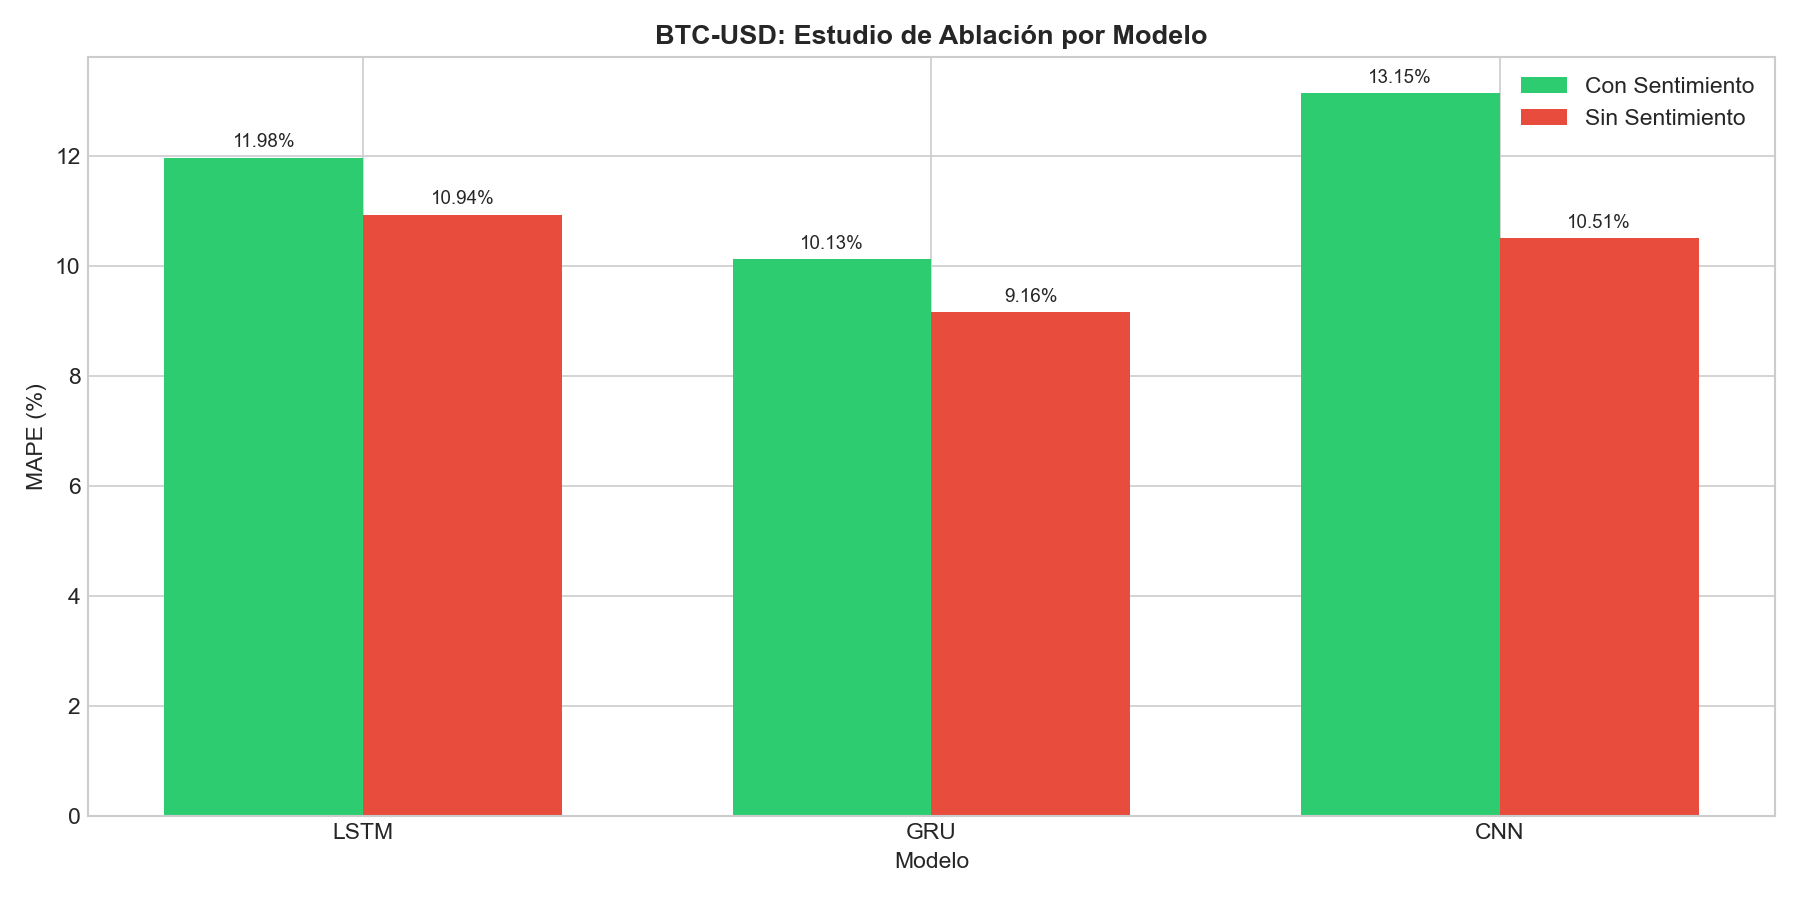
\includegraphics[width=0.90\textwidth]{Imagenes/ablation_BTC_USD_all_models.png}
\caption{BTC-USD: Ablación por modelo. En los tres modelos, incluir sentimiento empeora el MAPE (especialmente en CNN).}
\label{fig:ablation_btc}
\end{figure}

\begin{figure}[H]
\centering
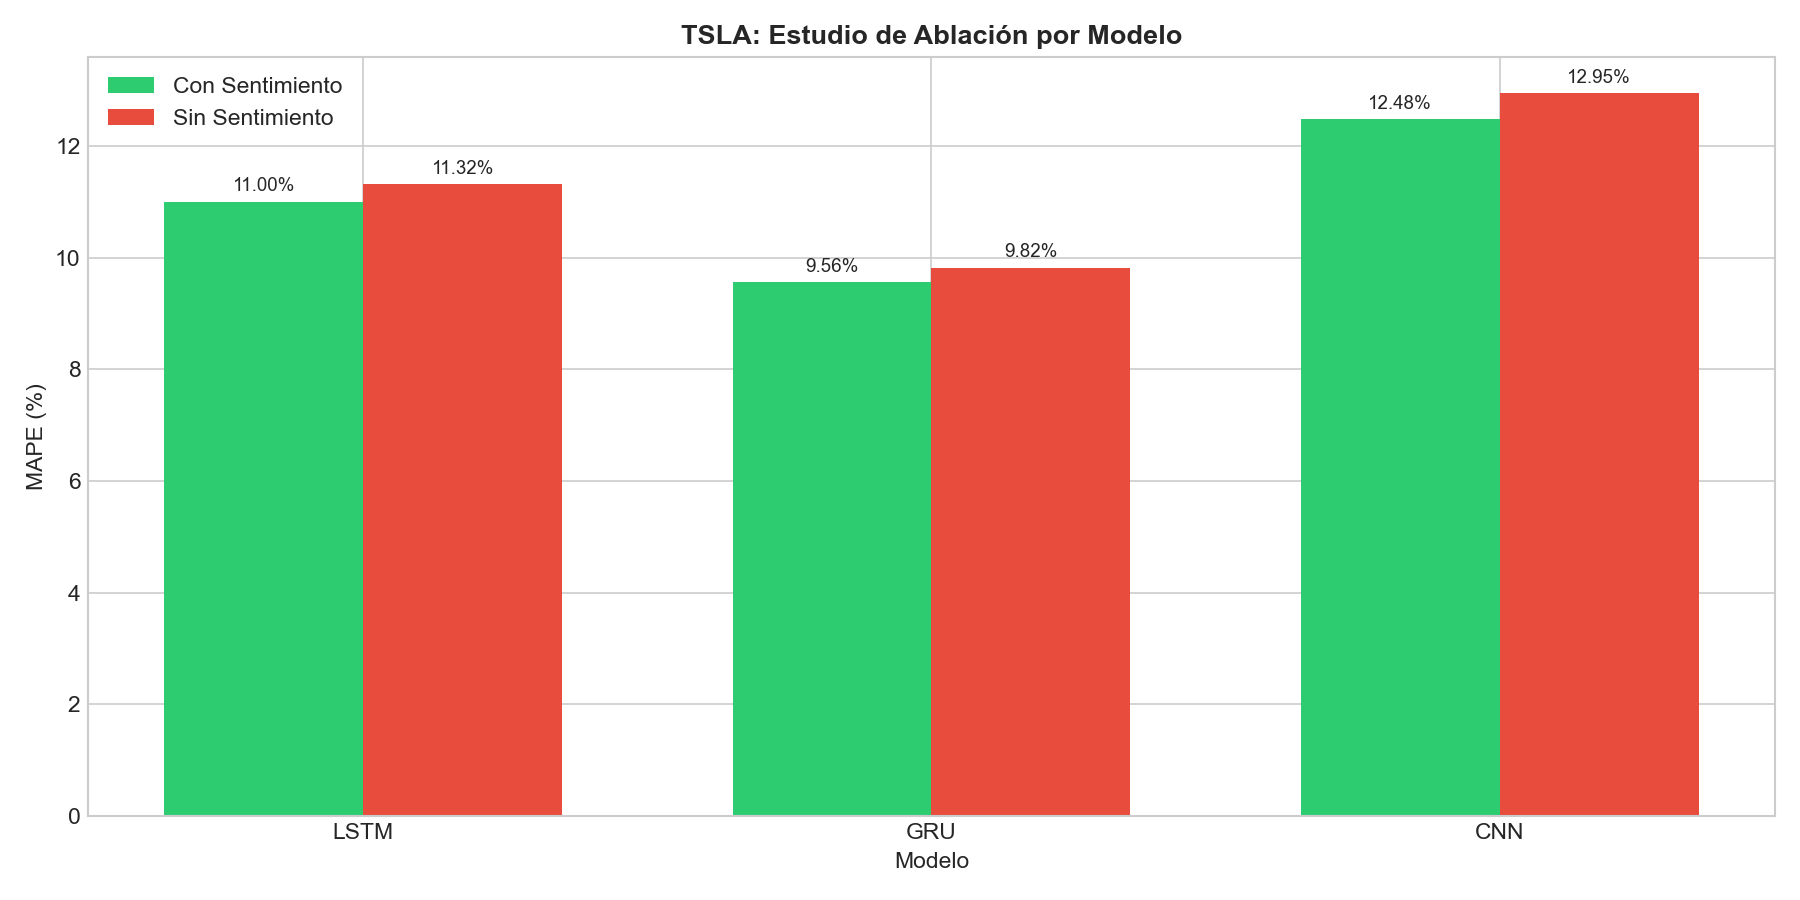
\includegraphics[width=0.90\textwidth]{Imagenes/ablation_TSLA_all_models.png}
\caption{TSLA: Ablación por modelo. Incluir sentimiento reduce el MAPE en los tres modelos, con mejoras pequeñas ($\sim$2--4\%).}
\label{fig:ablation_tsla}
\end{figure}

\begin{figure}[H]
\centering
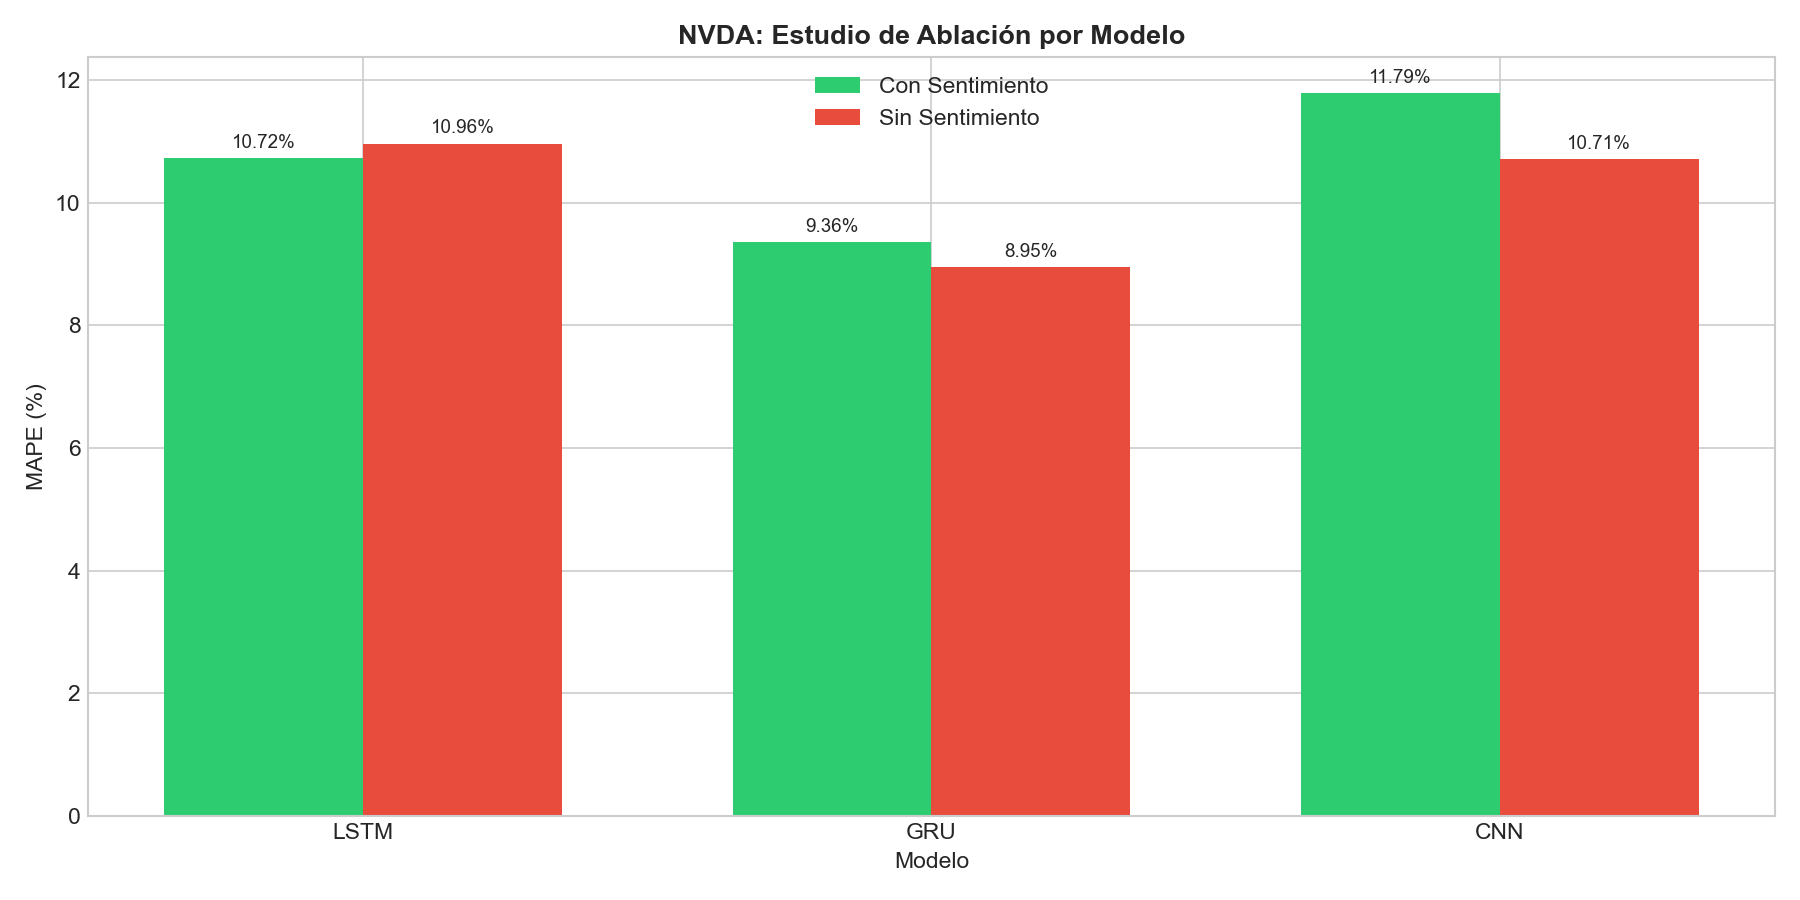
\includegraphics[width=0.90\textwidth]{Imagenes/ablation_NVDA_all_models.png}
\caption{NVDA: Ablación por modelo. LSTM mejora ligeramente; CNN y GRU empeoran.}
\label{fig:ablation_nvda}
\end{figure}

\begin{figure}[H]
\centering
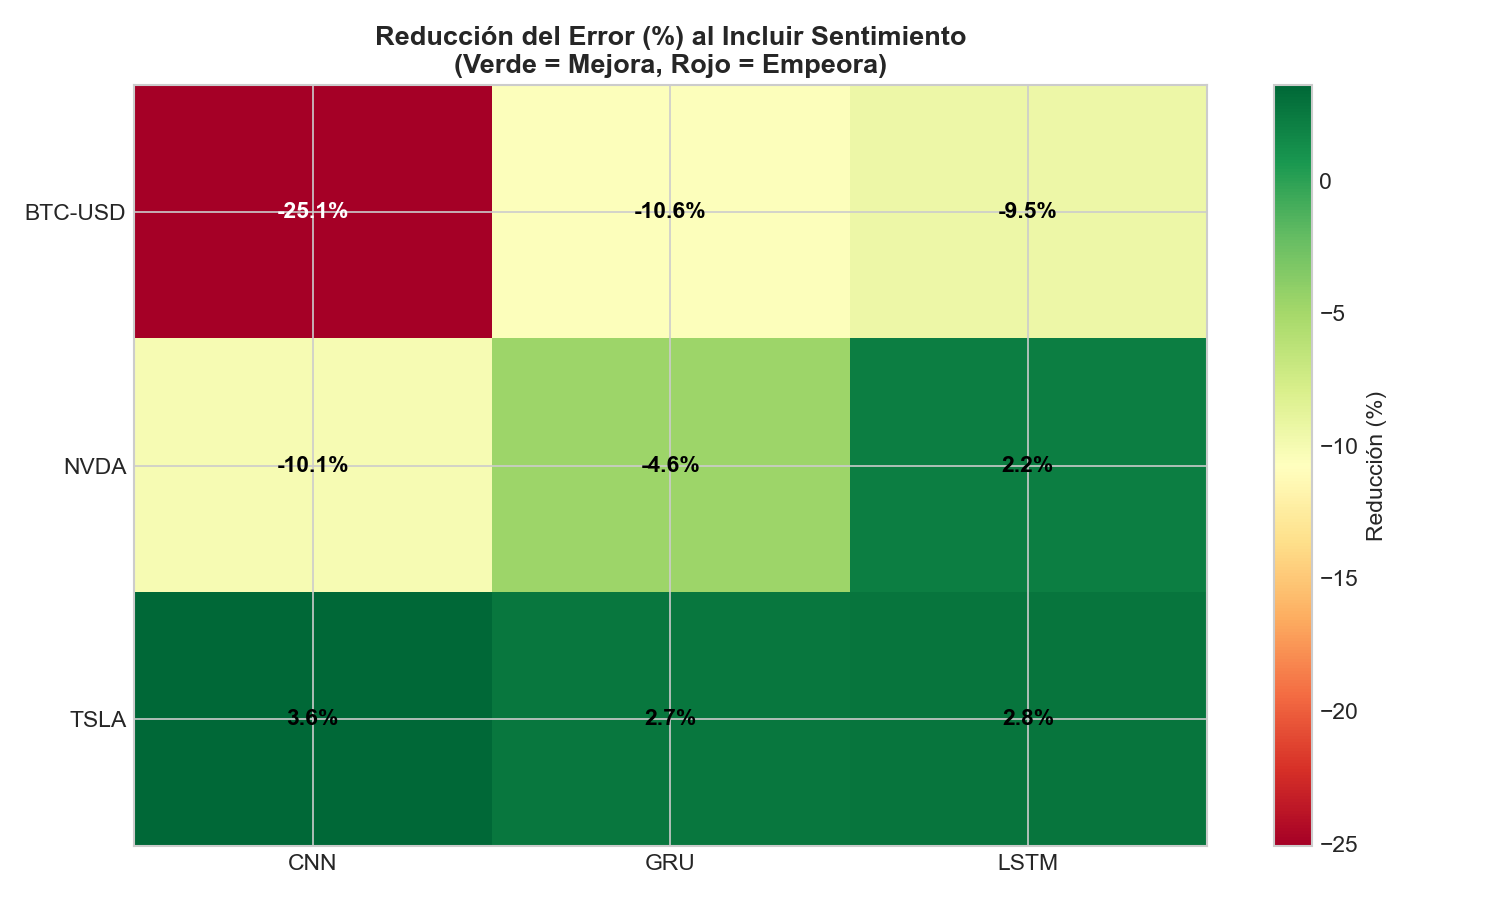
\includegraphics[width=0.90\textwidth]{Imagenes/ablation_improvement_heatmap.png}
\caption{Mapa de calor: Reducción del error (\%) al incluir sentimiento. Valores positivos (verdes) indican mejora; negativos (rojos) indican que el sentimiento perjudica.}
\label{fig:ablation_heatmap}
\end{figure}

Para ver el efecto desde el punto de vista de cada arquitectura, la Figura~\ref{fig:ablation_models_overview} resume la ablación por modelo en los tres activos.

\begin{figure}[H]
\centering
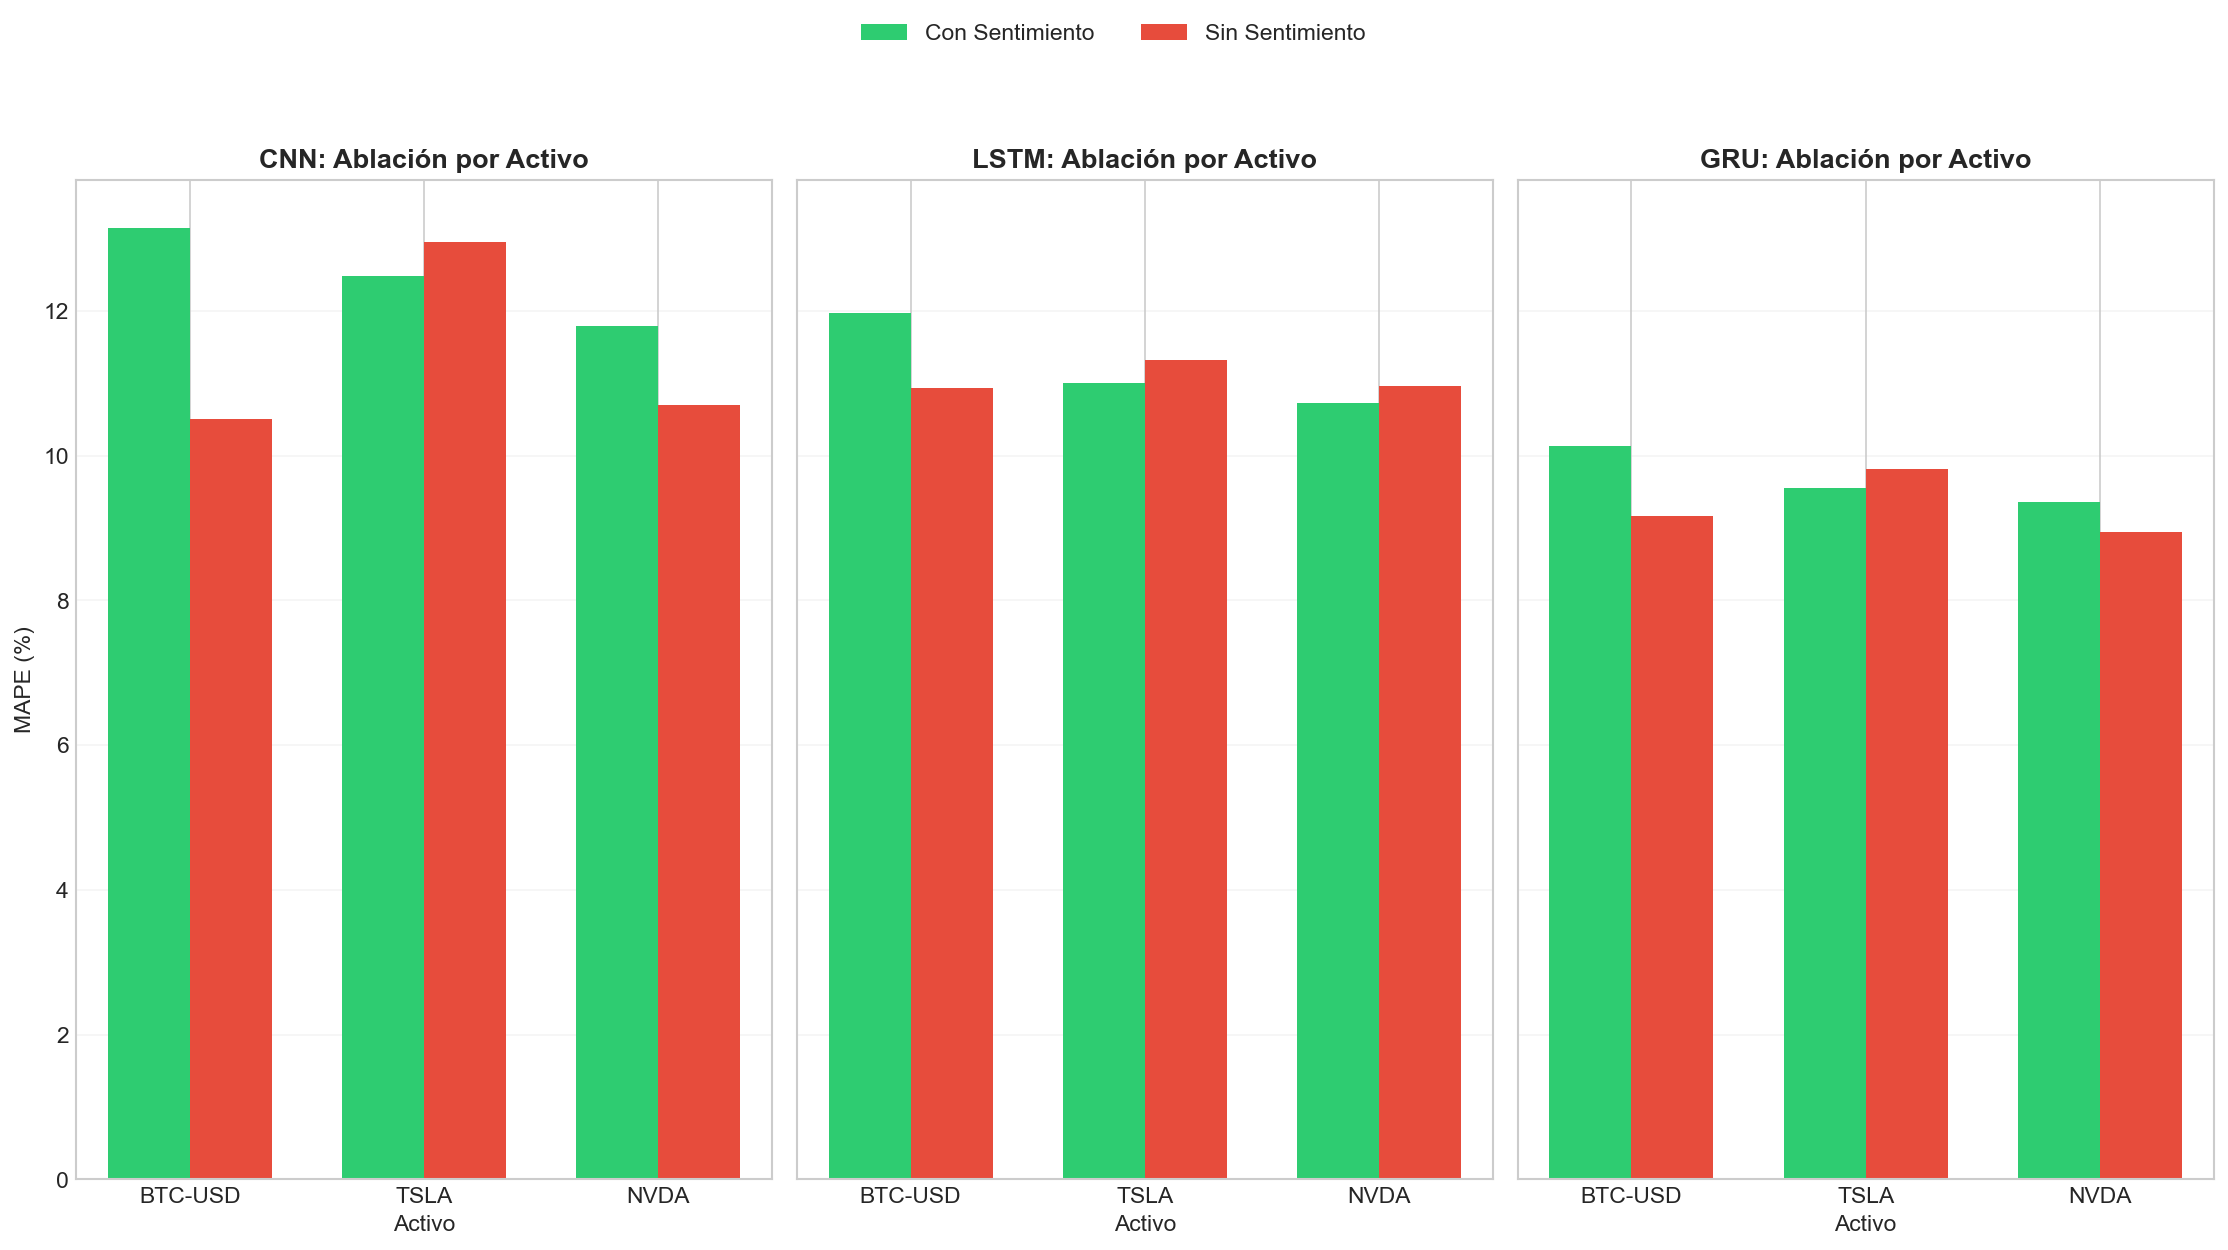
\includegraphics[width=0.95\textwidth]{Imagenes/ablation_models_overview.png}
\caption{Ablación por modelo (MAPE) comparando los tres activos.}
\label{fig:ablation_models_overview}
\end{figure}

En términos prácticos, esto significa que el sentimiento no es una ``mejora automática''. En Tesla aporta de forma consistente (aunque poco), mientras que en Bitcoin y, salvo en el caso de LSTM en Nvidia, tiende a perjudicar. La conclusión no es que el sentimiento carezca de utilidad, sino que su contribución se limita a determinadas condiciones.

\subsection{Significancia estadística de la ablación}

Además de comparar medias, se aplicó un test de Wilcoxon pareado sobre las métricas por fold para evaluar si la diferencia con/sin sentimiento es consistente. La Tabla~\ref{tab:ablation_tests} resume los resultados para MAPE y métricas direccionales (DA, F1 y MCC). En la tabla, la columna \textbf{Dif.} se define como \textbf{(sin sentimiento) $-$ (con sentimiento)}: en MAPE un valor positivo indica que incluir sentimiento reduce el error (mejora), mientras que en las métricas direccionales un valor positivo indica mejor comportamiento sin sentimiento.

\begin{table}[H]
\centering
\caption{Test de Wilcoxon para la ablación con/sin sentimiento}
\label{tab:ablation_tests}
\begin{tabular}{l|l|c|c|c|c}
\hline
\textbf{Activo} & \textbf{Modelo} & \textbf{Metr.} & \textbf{Dif.} & \textbf{p} & \textbf{Sig.?} \\
\hline
BTC-USD & CNN & MAPE & -2.64 & 0.233 & No \\
BTC-USD & GRU & MAPE & -0.97 & 1.000 & No \\
BTC-USD & LSTM & MAPE & -1.04 & 0.733 & No \\
NVDA & CNN & MAPE & -1.08 & 0.110 & No \\
NVDA & GRU & MAPE & -0.41 & 0.424 & No \\
NVDA & LSTM & MAPE & 0.24 & 0.470 & No \\
TSLA & CNN & MAPE & 0.47 & 0.380 & No \\
TSLA & GRU & MAPE & 0.26 & 0.470 & No \\
TSLA & LSTM & MAPE & 0.32 & 0.176 & No \\
BTC-USD & CNN & DA & 1.11 & 0.766 & No \\
BTC-USD & GRU & DA & 2.50 & 0.461 & No \\
BTC-USD & LSTM & DA & -1.94 & 0.688 & No \\
NVDA & CNN & DA & 2.50 & 0.508 & No \\
NVDA & GRU & DA & 0.56 & 1.000 & No \\
NVDA & LSTM & DA & -1.67 & 0.469 & No \\
TSLA & CNN & DA & -3.89 & 0.336 & No \\
TSLA & GRU & DA & 1.11 & 0.625 & No \\
TSLA & LSTM & DA & -0.28 & 0.844 & No \\
BTC-USD & CNN & F1 & 7.02 & 0.461 & No \\
BTC-USD & GRU & F1 & 7.37 & 0.164 & No \\
BTC-USD & LSTM & F1 & 3.03 & 0.742 & No \\
NVDA & CNN & F1 & 8.78 & 0.278 & No \\
NVDA & GRU & F1 & 1.07 & 0.812 & No \\
NVDA & LSTM & F1 & -3.11 & 0.461 & No \\
TSLA & CNN & F1 & -9.52 & 0.206 & No \\
TSLA & GRU & F1 & 2.21 & 0.312 & No \\
TSLA & LSTM & F1 & 0.68 & 0.688 & No \\
BTC-USD & CNN & MCC & -0.02 & 0.652 & No \\
BTC-USD & GRU & MCC & 0.00 & 0.910 & No \\
BTC-USD & LSTM & MCC & -0.00 & 0.742 & No \\
NVDA & CNN & MCC & 0.12 & 0.024 & Si \\
NVDA & GRU & MCC & -0.03 & 0.812 & No \\
NVDA & LSTM & MCC & 0.01 & 0.945 & No \\
TSLA & CNN & MCC & -0.08 & 0.465 & No \\
TSLA & GRU & MCC & 0.03 & 0.688 & No \\
TSLA & LSTM & MCC & 0.05 & 0.297 & No \\
\hline
\end{tabular}
\end{table}

La Figura~\ref{fig:wilcoxon_pvalues} ofrece una lectura rápida de los p-values: cuanto más oscuro, más evidencia contra la hipótesis nula.

\begin{figure}[H]
\centering
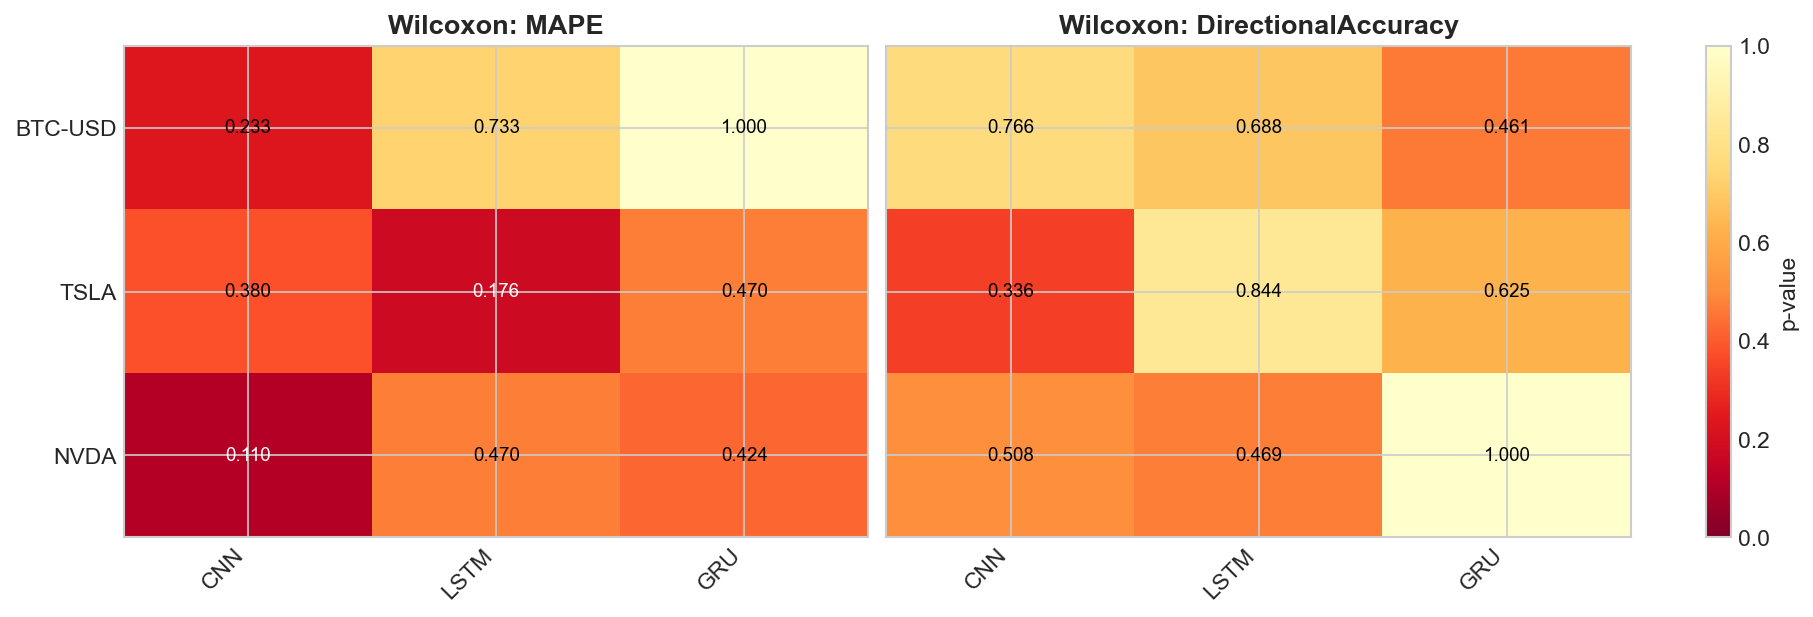
\includegraphics[width=0.95\textwidth]{Imagenes/wilcoxon_pvalues_heatmap.png}
\caption{P-values del test de Wilcoxon para MAPE y precisión direccional.}
\label{fig:wilcoxon_pvalues}
\end{figure}

En MAPE y en DA/F1 no aparecen diferencias significativas (p < 0.05) en ninguna combinación. Solo aparece un caso aislado significativo en MCC (NVDA-CNN), por lo que no cambia la conclusión general. El signo de \textbf{Dif.} sugiere tendencias (por ejemplo, que el sentimiento tiende a empeorar el MAPE en Bitcoin y a mejorar ligeramente en Tesla), pero el efecto no es estadísticamente consistente por fold.

En síntesis, no hay evidencia sólida de que el error baje de forma repetible al incluir sentimiento. Eso pone límites a cualquier conclusión contundente y es coherente con la variabilidad que se observa en la ablación.

Implicación práctica: incluir sentimiento tiene un coste (datos y procesamiento) y solo se justifica cuando la mejora es clara, estable y repetible. En este estudio, aunque Tesla muestra un patrón favorable, el tamaño del efecto es pequeño y no alcanza significancia estadística.

%% ============================================================
%% EXPERIMENTO D: PERIODOS DE MERCADO
%% ============================================================

\section{Rendimiento por periodos de mercado}

El último experimento compara el rendimiento de los tres modelos de aprendizaje profundo (LSTM, GRU y CNN) en tres periodos muy diferentes para Bitcoin.

\subsection{Los números}

La Tabla~\ref{tab:experiment_d} recoge las métricas de cada modelo en los tres periodos, y la Figura~\ref{fig:market_periods} las visualiza.

\begin{table}[H]
\centering
\caption{Rendimiento de LSTM, GRU y CNN por periodo de mercado (BTC-USD, h=7)}
\label{tab:experiment_d}
\begin{tabular}{l|l|ccc}
\hline
\textbf{Periodo} & \textbf{Modelo} & \textbf{RMSE (USD)} & \textbf{MAE (USD)} & \textbf{MAPE (\%)} \\
\hline
Bull-2021 & LSTM & 8513 & 7184 & 11.99 \\
Bull-2021 & GRU & 6336 & 5165 & 8.71 \\
Bull-2021 & CNN & 9405 & 7577 & 12.64 \\
Bear-2022 & LSTM & 1571 & 1143 & 6.50 \\
Bear-2022 & GRU & 1816 & 1368 & 7.41 \\
Bear-2022 & CNN & 1642 & 1258 & 7.13 \\
Recent & LSTM & 6868 & 5451 & 4.86 \\
Recent & GRU & 5180 & 4085 & 3.71 \\
Recent & CNN & 8482 & 7050 & 6.48 \\
\hline
\end{tabular}
\end{table}

\begin{figure}[H]
\centering
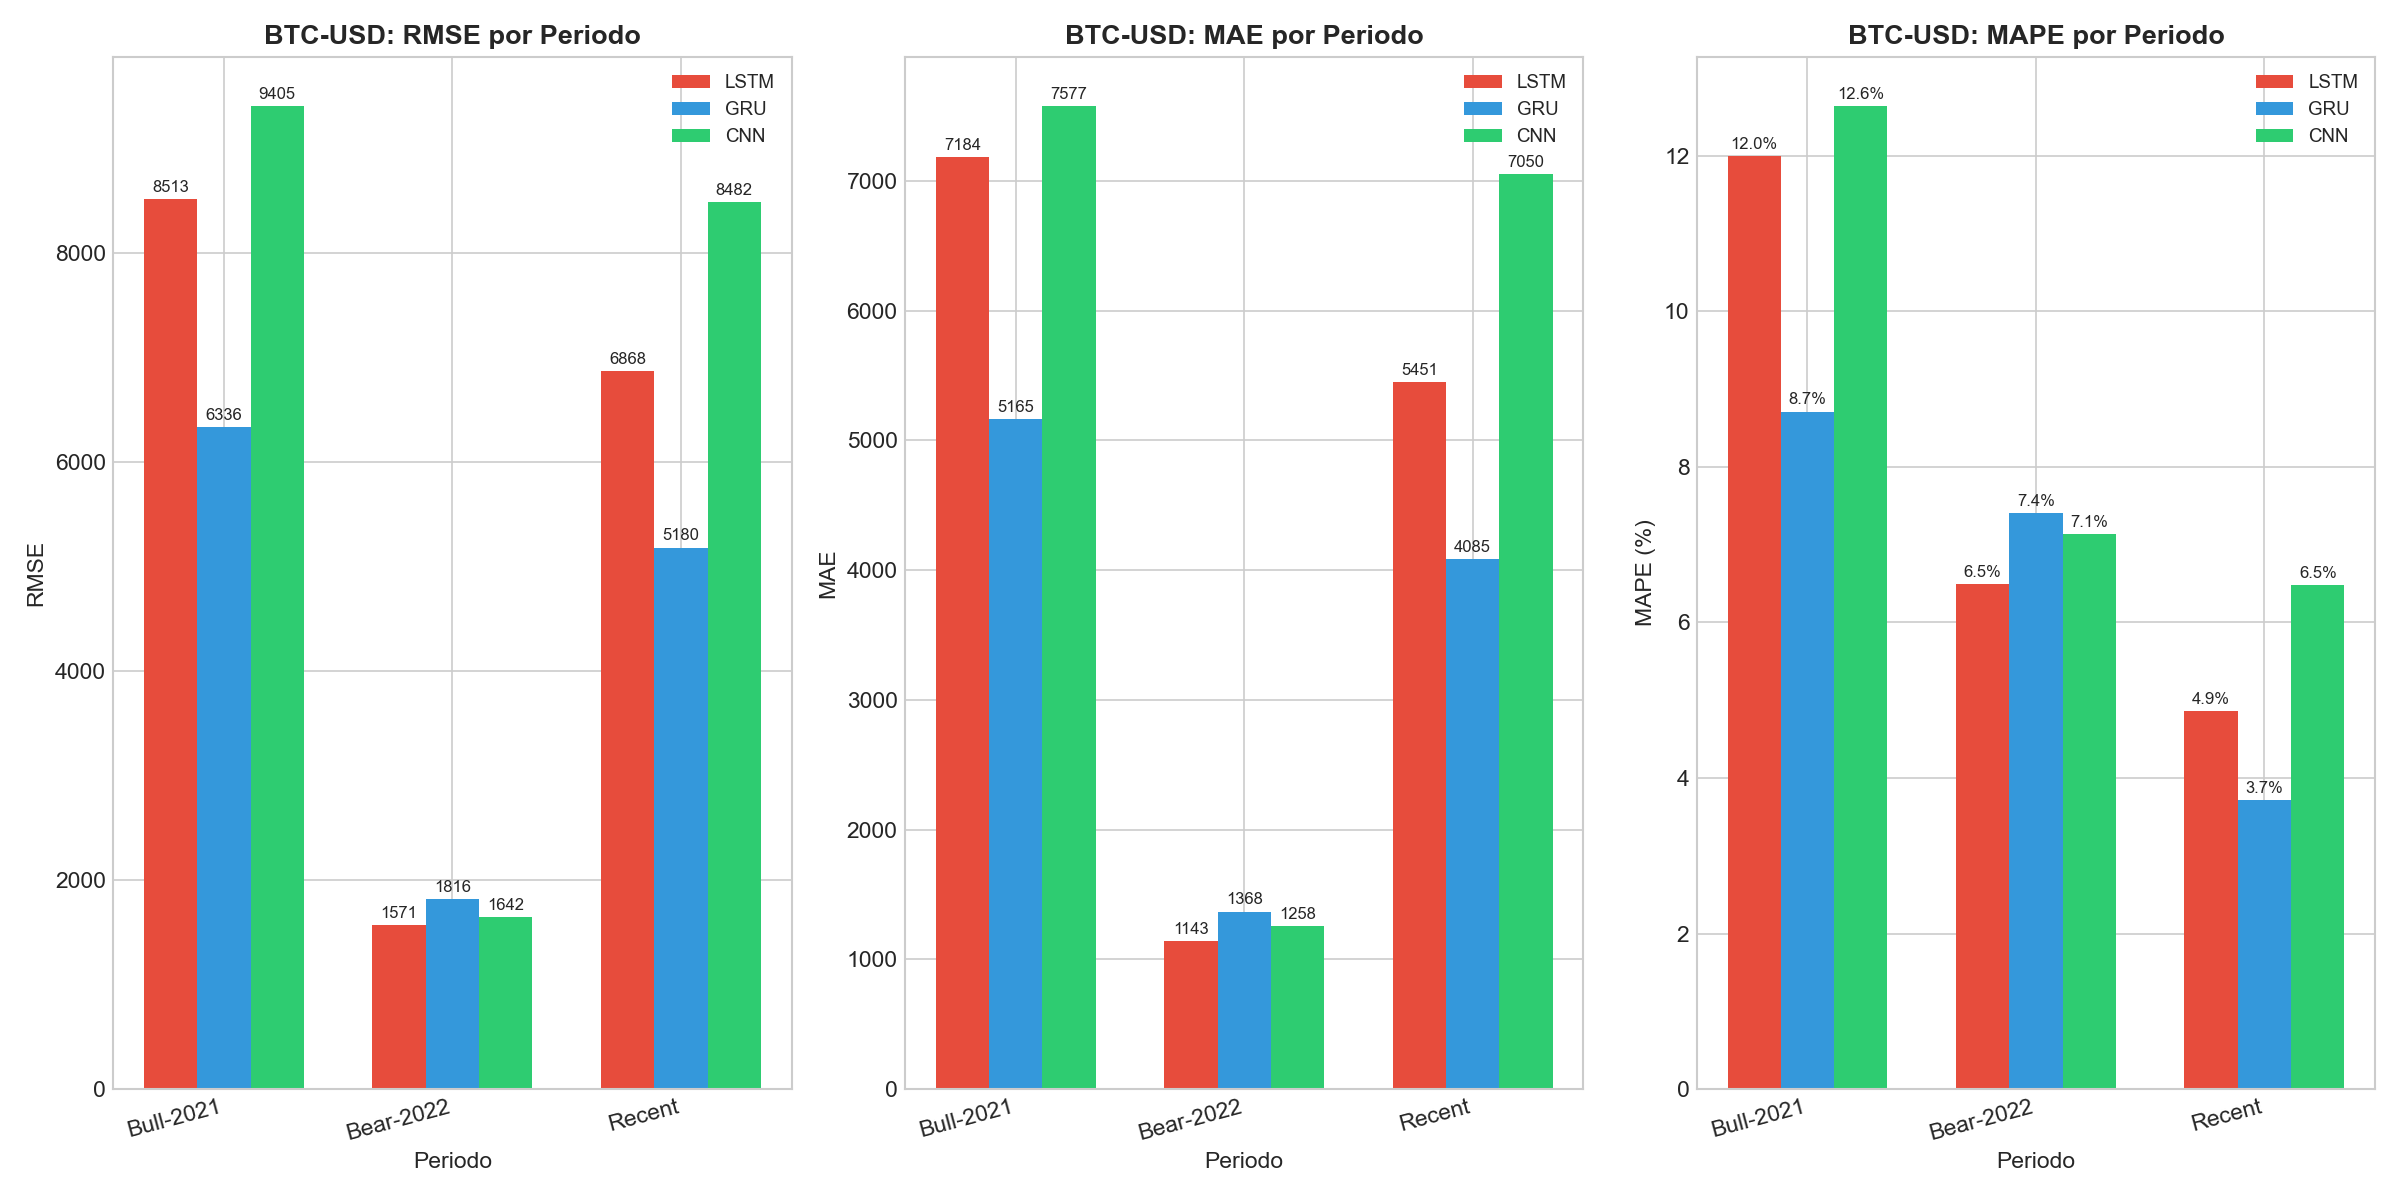
\includegraphics[width=0.95\textwidth]{Imagenes/market_periods_all_metrics.png}
\caption{Rendimiento por periodo de mercado para los tres modelos DL.}
\label{fig:market_periods}
\end{figure}

El rendimiento varía sustancialmente entre periodos y entre modelos. En el periodo alcista de 2021, GRU es claramente el mejor modelo (MAPE 8.71\%), mientras que LSTM (11.99\%) y CNN (12.64\%) quedan lejos. En el mercado bajista de 2022, las diferencias se reducen: LSTM obtiene el menor MAPE (6.50\%), seguido de CNN (7.13\%) y GRU (7.41\%). En el periodo reciente, GRU vuelve a liderar con un MAPE de 3.71\%, seguido de LSTM (4.86\%) y CNN (6.48\%).

Este resultado tiene varias lecturas. Primero, GRU es la arquitectura más consistente en dos de los tres periodos y la que mejor MAPE global presenta. Segundo, respecto al tramo alcista de 2021, el rendimiento en el mercado bajista de 2022 mejora para los tres modelos en MAPE, lo que puede parecer contraintuitivo; sin embargo, los precios absolutos eran significativamente menores, lo que reduce el error relativo. Tercero, CNN muestra una consistencia intermedia pero es la más inestable en direccionalidad: en el periodo reciente apenas alcanza un 37.5\% de precisión direccional, lo que es peor que el azar.

Por tanto, el rendimiento de un mismo modelo puede variar sustancialmente entre periodos, incluso con hiperparámetros constantes. Esta sensibilidad al régimen es una limitación práctica que conviene explicitar. Además, las diferencias entre arquitecturas se amplifican en ciertos regímenes, lo que sugiere que la elección del modelo no es independiente del contexto de mercado.

Implicación práctica: si se usa un modelo para apoyar decisiones, hay que vigilar el contexto de mercado y considerar que el ranking entre LSTM, GRU y CNN puede cambiar según el régimen. GRU parece la opción más segura como punto de partida, pero LSTM puede superarlo en entornos bajistas.

%% ============================================================
%% PREDICCIONES VS VALORES REALES
%% ============================================================

\section{Análisis cualitativo de predicciones}

Las tablas resumen métricas agregadas, mientras que las figuras permiten evaluar la dinámica del ajuste. En esta sección se muestran las predicciones superpuestas con los valores reales para cada activo y horizonte.

La idea no es buscar coincidencia punto a punto, sino ver si el modelo sigue la tendencia general y qué tipo de errores comete: desfases, suavizado de picos o incapacidad para reaccionar a shocks.

Estas gráficas se generan con el conjunto completo de variables, incluyendo sentimiento; es decir, corresponden a la versión ``con sentimiento'' del modelo.

\subsection{Bitcoin}

\begin{figure}[H]
\centering
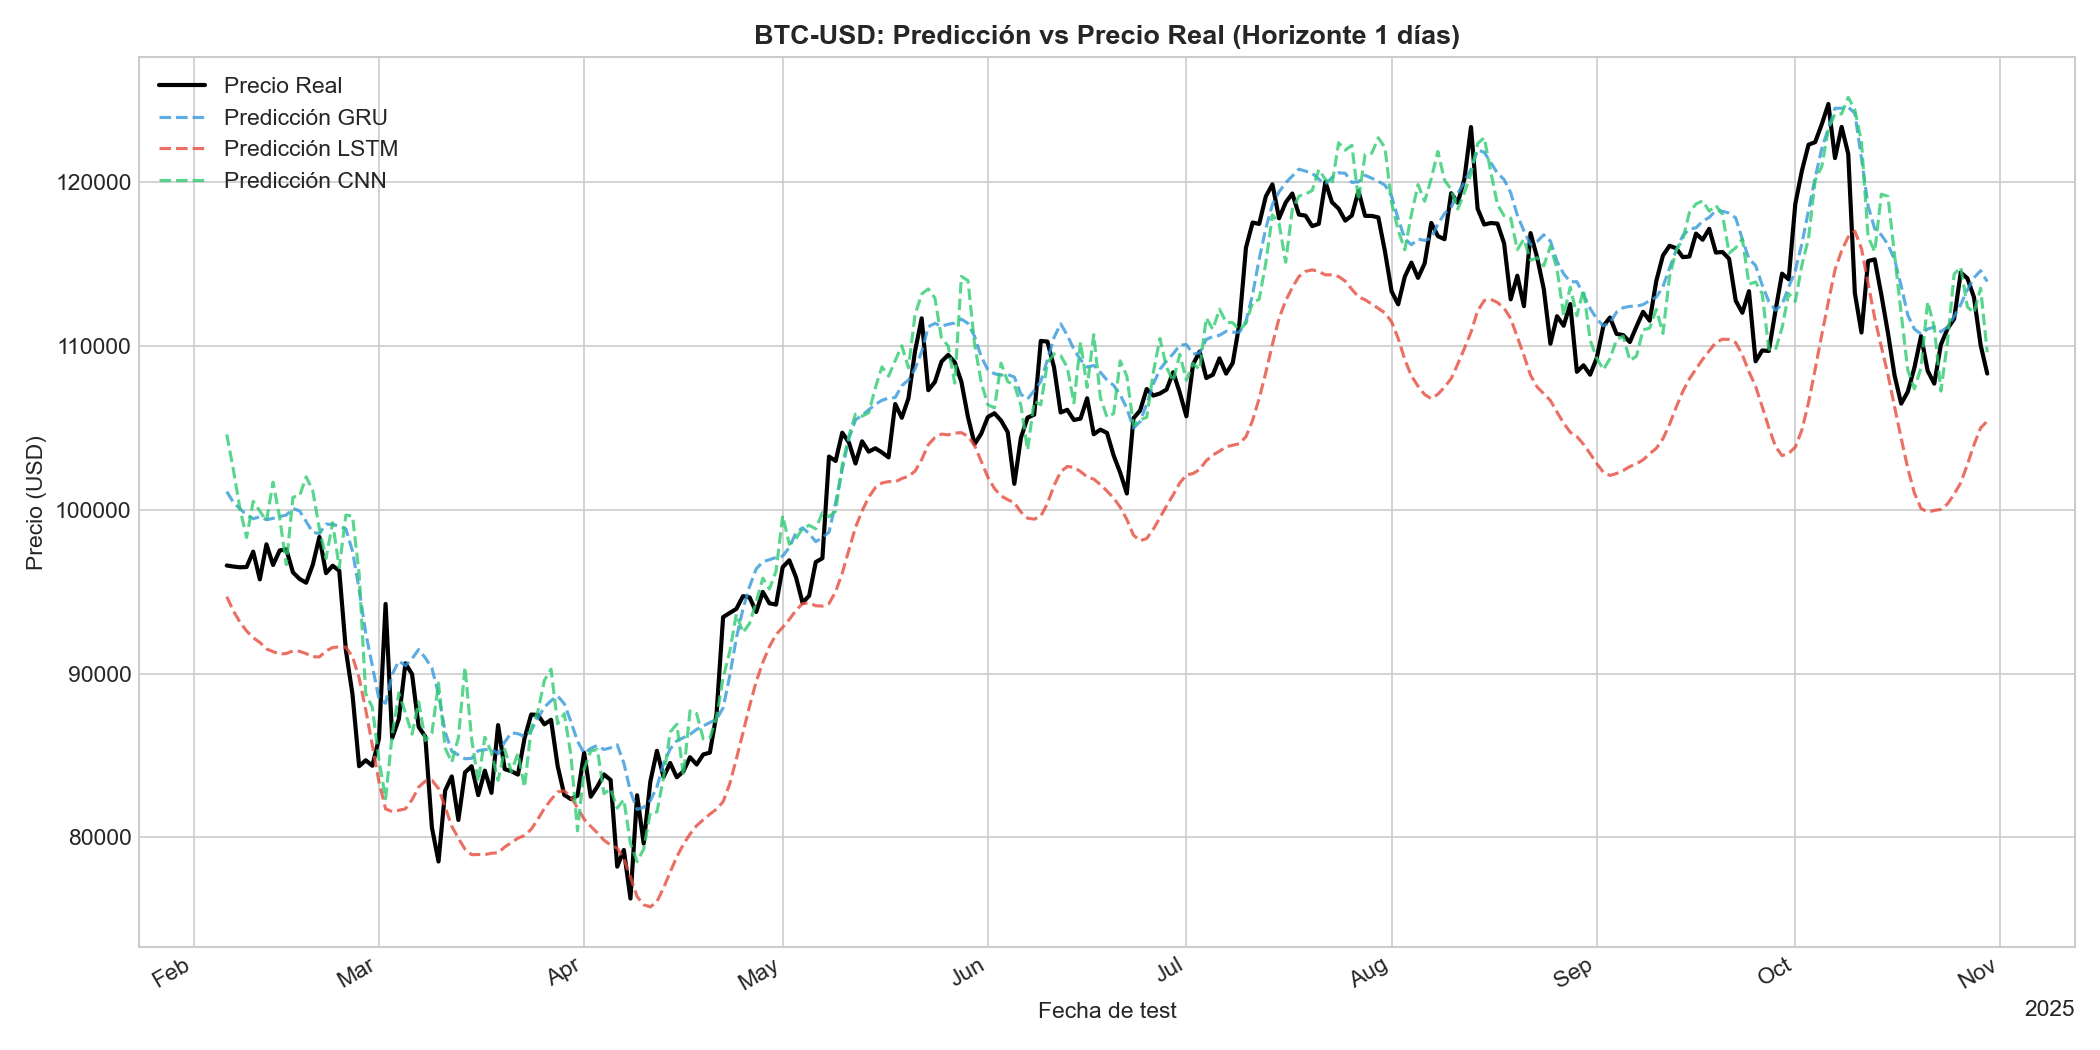
\includegraphics[width=0.95\textwidth]{Imagenes/pred_vs_actual_BTC_USD_h1.png}
\caption{BTC-USD: Predicción vs Real (1 día). A horizonte de un día, el modelo sigue de cerca la serie real, aunque con un ligero retardo. Las predicciones tienden a suavizar los picos, lo que es típico de modelos que aprenden de ventanas históricas.}
\label{fig:pred_btc_h1}
\end{figure}

\begin{figure}[H]
\centering
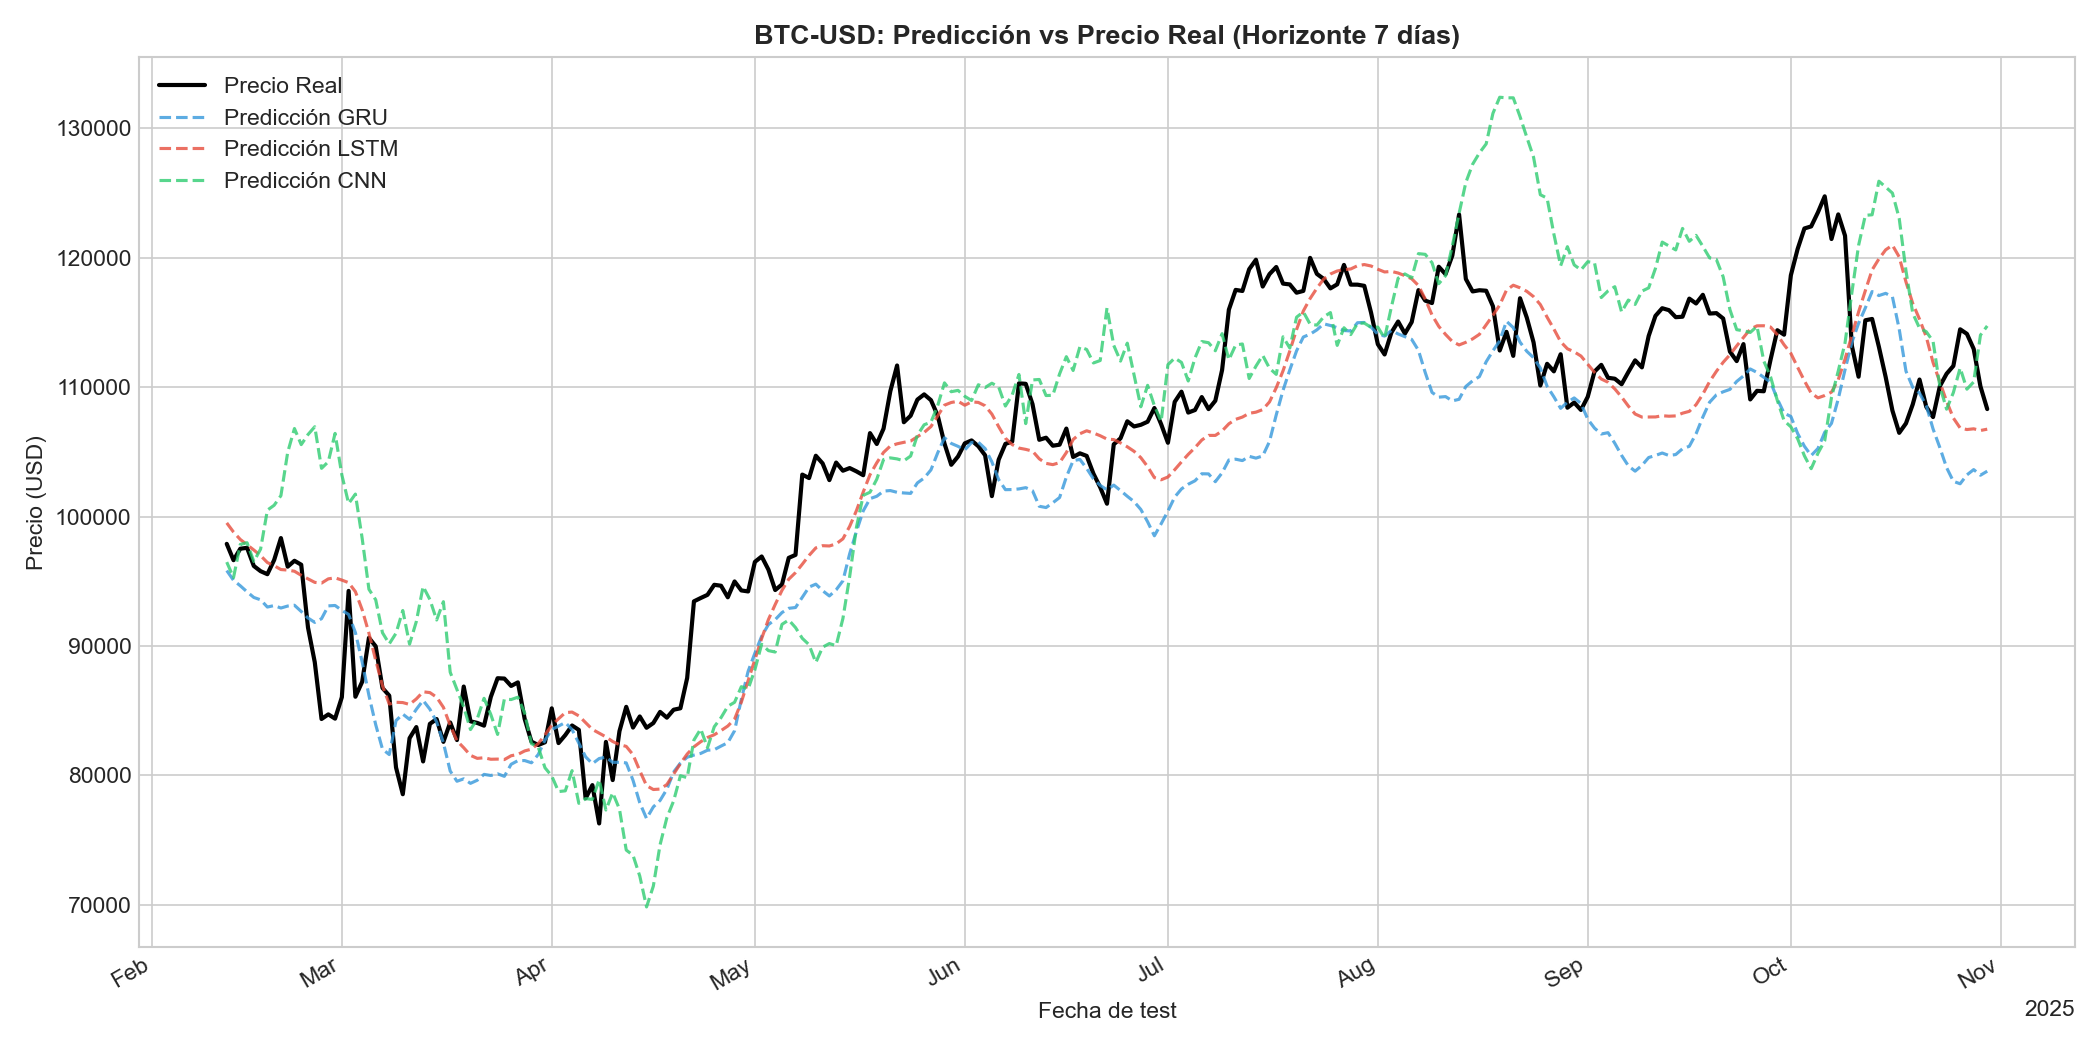
\includegraphics[width=0.95\textwidth]{Imagenes/pred_vs_actual_BTC_USD_h7.png}
\caption{BTC-USD: Predicción vs Real (7 días). Con una semana de horizonte, el error aumenta pero la tendencia general sigue siendo reconocible. Los cambios bruscos de dirección son los que mayor error generan, ya que el modelo no puede anticipar eventos inesperados.}
\label{fig:pred_btc_h7}
\end{figure}

\begin{figure}[H]
\centering
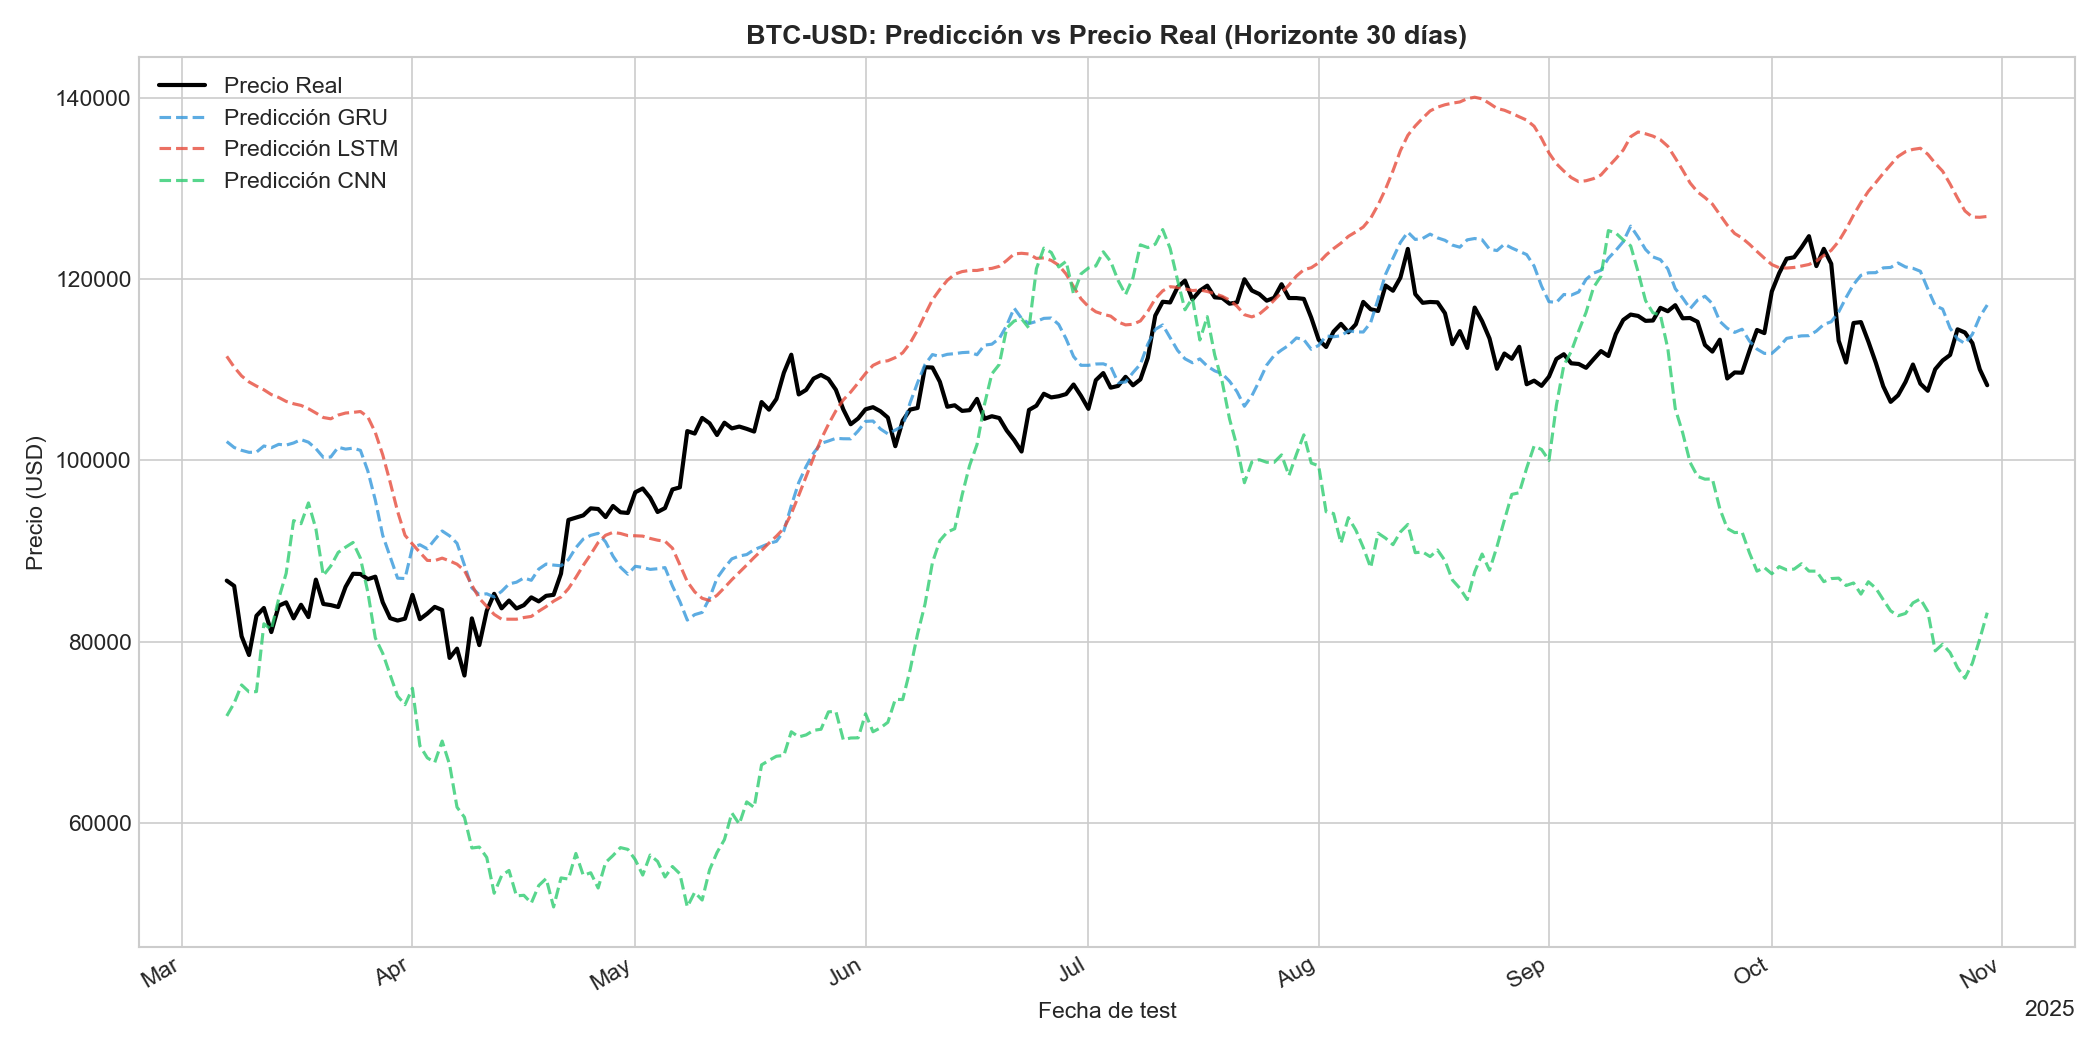
\includegraphics[width=0.95\textwidth]{Imagenes/pred_vs_actual_BTC_USD_h30.png}
\caption{BTC-USD: Predicción vs Real (30 días). A un mes, la predicción se convierte esencialmente en una media suavizada. El modelo captura la dirección general pero pierde resolución en los movimientos intermedios.}
\label{fig:pred_btc_h30}
\end{figure}

En conjunto, las gráficas de Bitcoin muestran un patrón consistente: las predicciones tienden a suavizar los movimientos y a llegar tarde a los cambios bruscos. Esto es habitual en modelos entrenados con ventanas históricas y refleja la dificultad intrínseca de anticipar shocks en un mercado tan volátil como el de criptomonedas. A medida que aumenta el horizonte, la curva de predicción se aplana progresivamente, lo que indica que el modelo pierde capacidad de seguimiento y converge hacia valores medios.

\clearpage
\subsection{Tesla}

\begin{figure}[H]
\centering
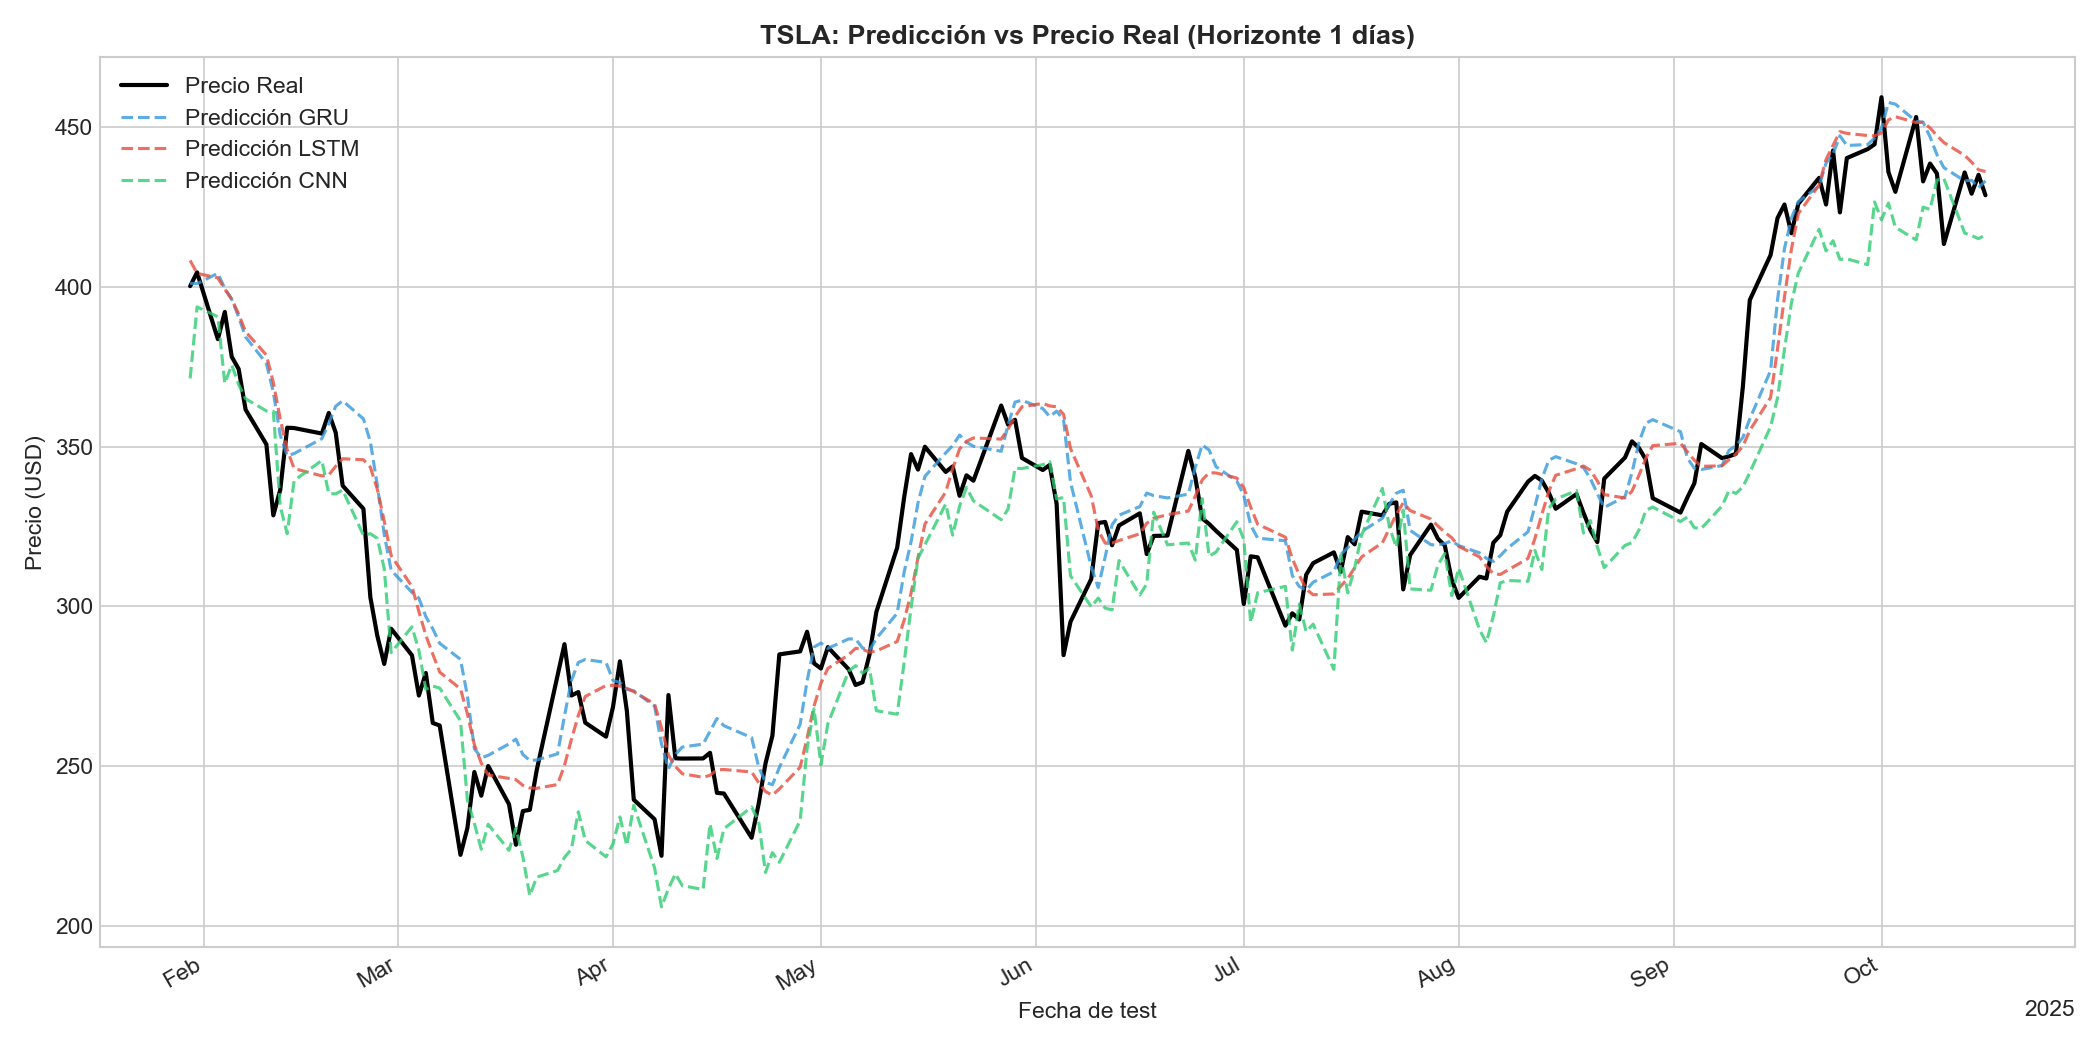
\includegraphics[width=0.95\textwidth]{Imagenes/pred_vs_actual_TSLA_h1.png}
\caption{TSLA: Predicción vs Real (1 día). Tesla muestra un ajuste visual más limpio que Bitcoin a corto plazo. El modelo captura la mayoría de movimientos diarios, aunque tiende a subestimar la magnitud de los picos más pronunciados.}
\label{fig:pred_tsla_h1}
\end{figure}

\begin{figure}[H]
\centering
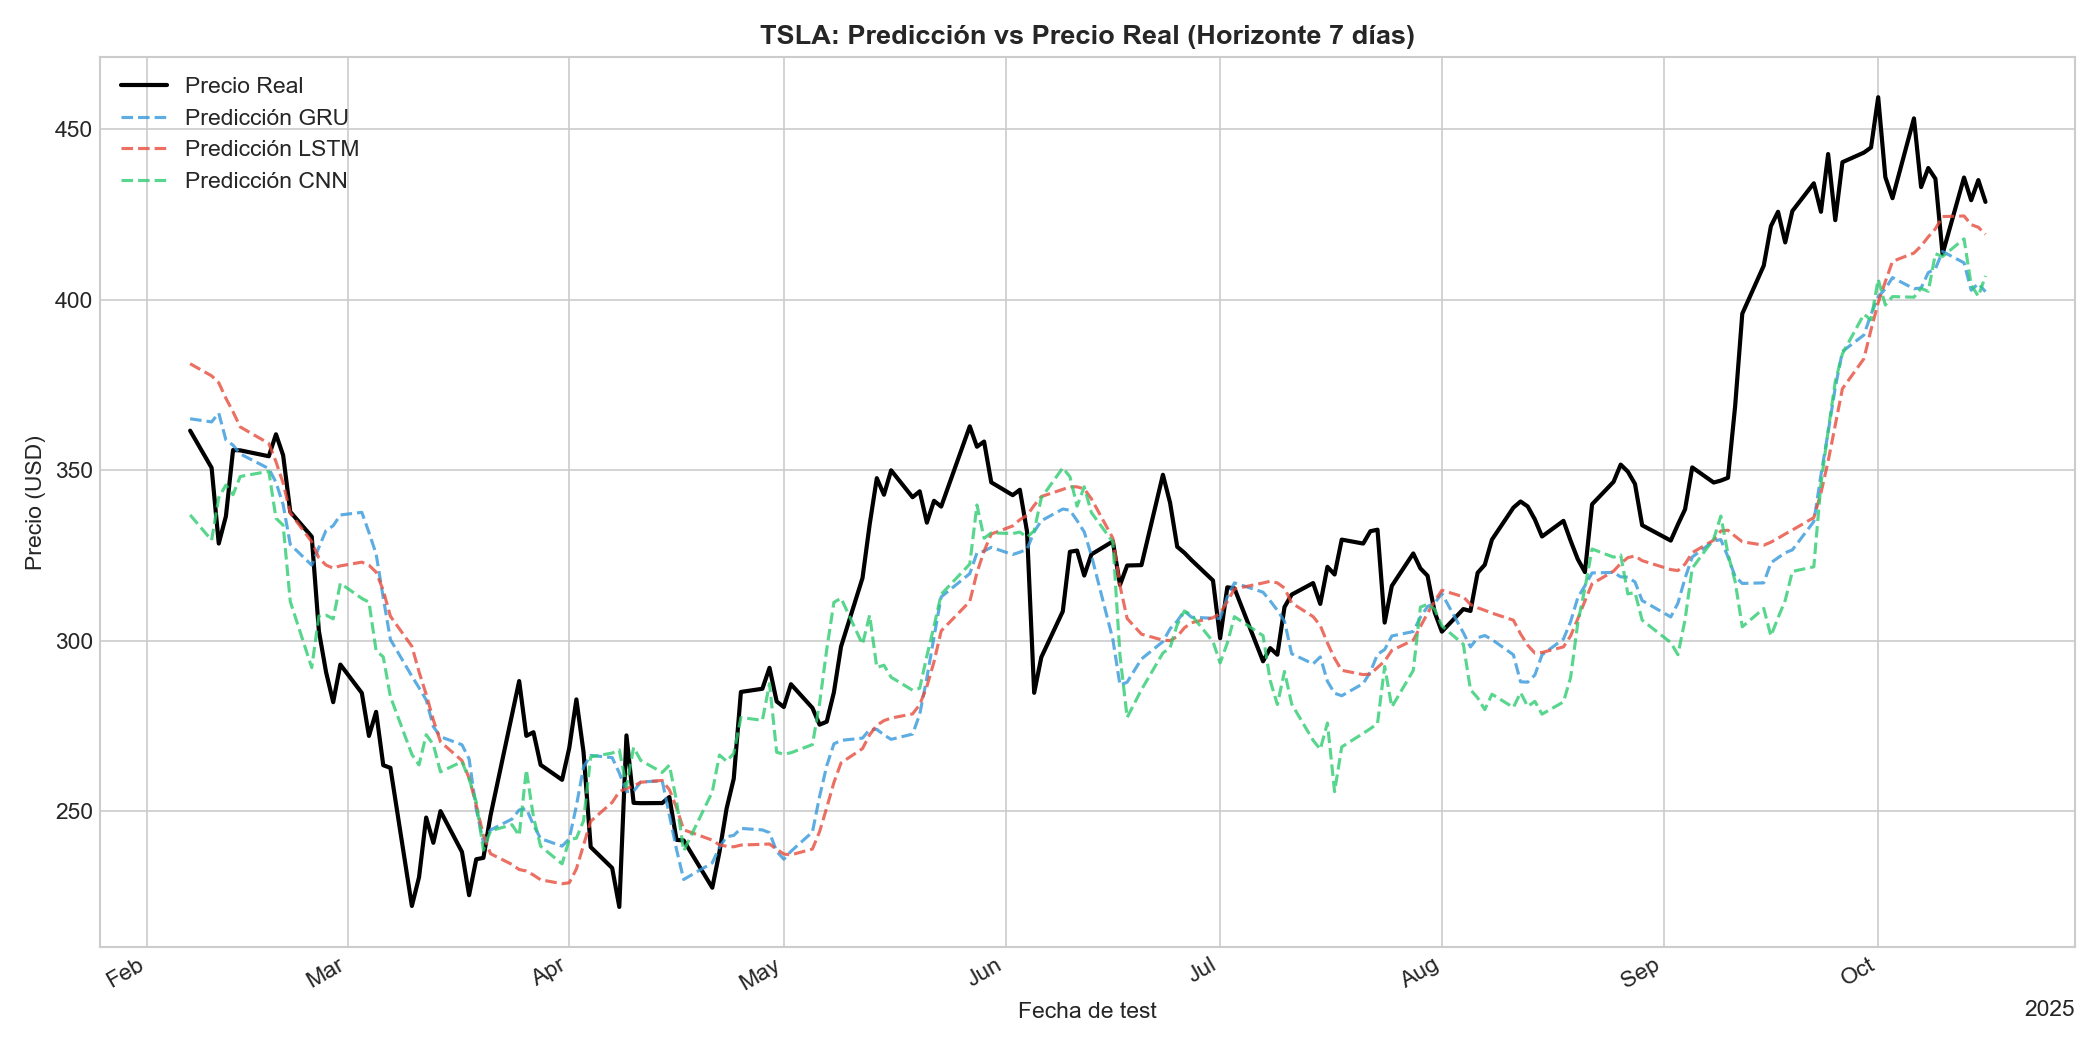
\includegraphics[width=0.95\textwidth]{Imagenes/pred_vs_actual_TSLA_h7.png}
\caption{TSLA: Predicción vs Real (7 días). A una semana, el modelo mantiene un seguimiento razonable de la tendencia, aunque los picos de volatilidad generan desviaciones significativas. Los periodos de baja volatilidad muestran mejor ajuste que los turbulentos.}
\label{fig:pred_tsla_h7}
\end{figure}

\begin{figure}[H]
\centering
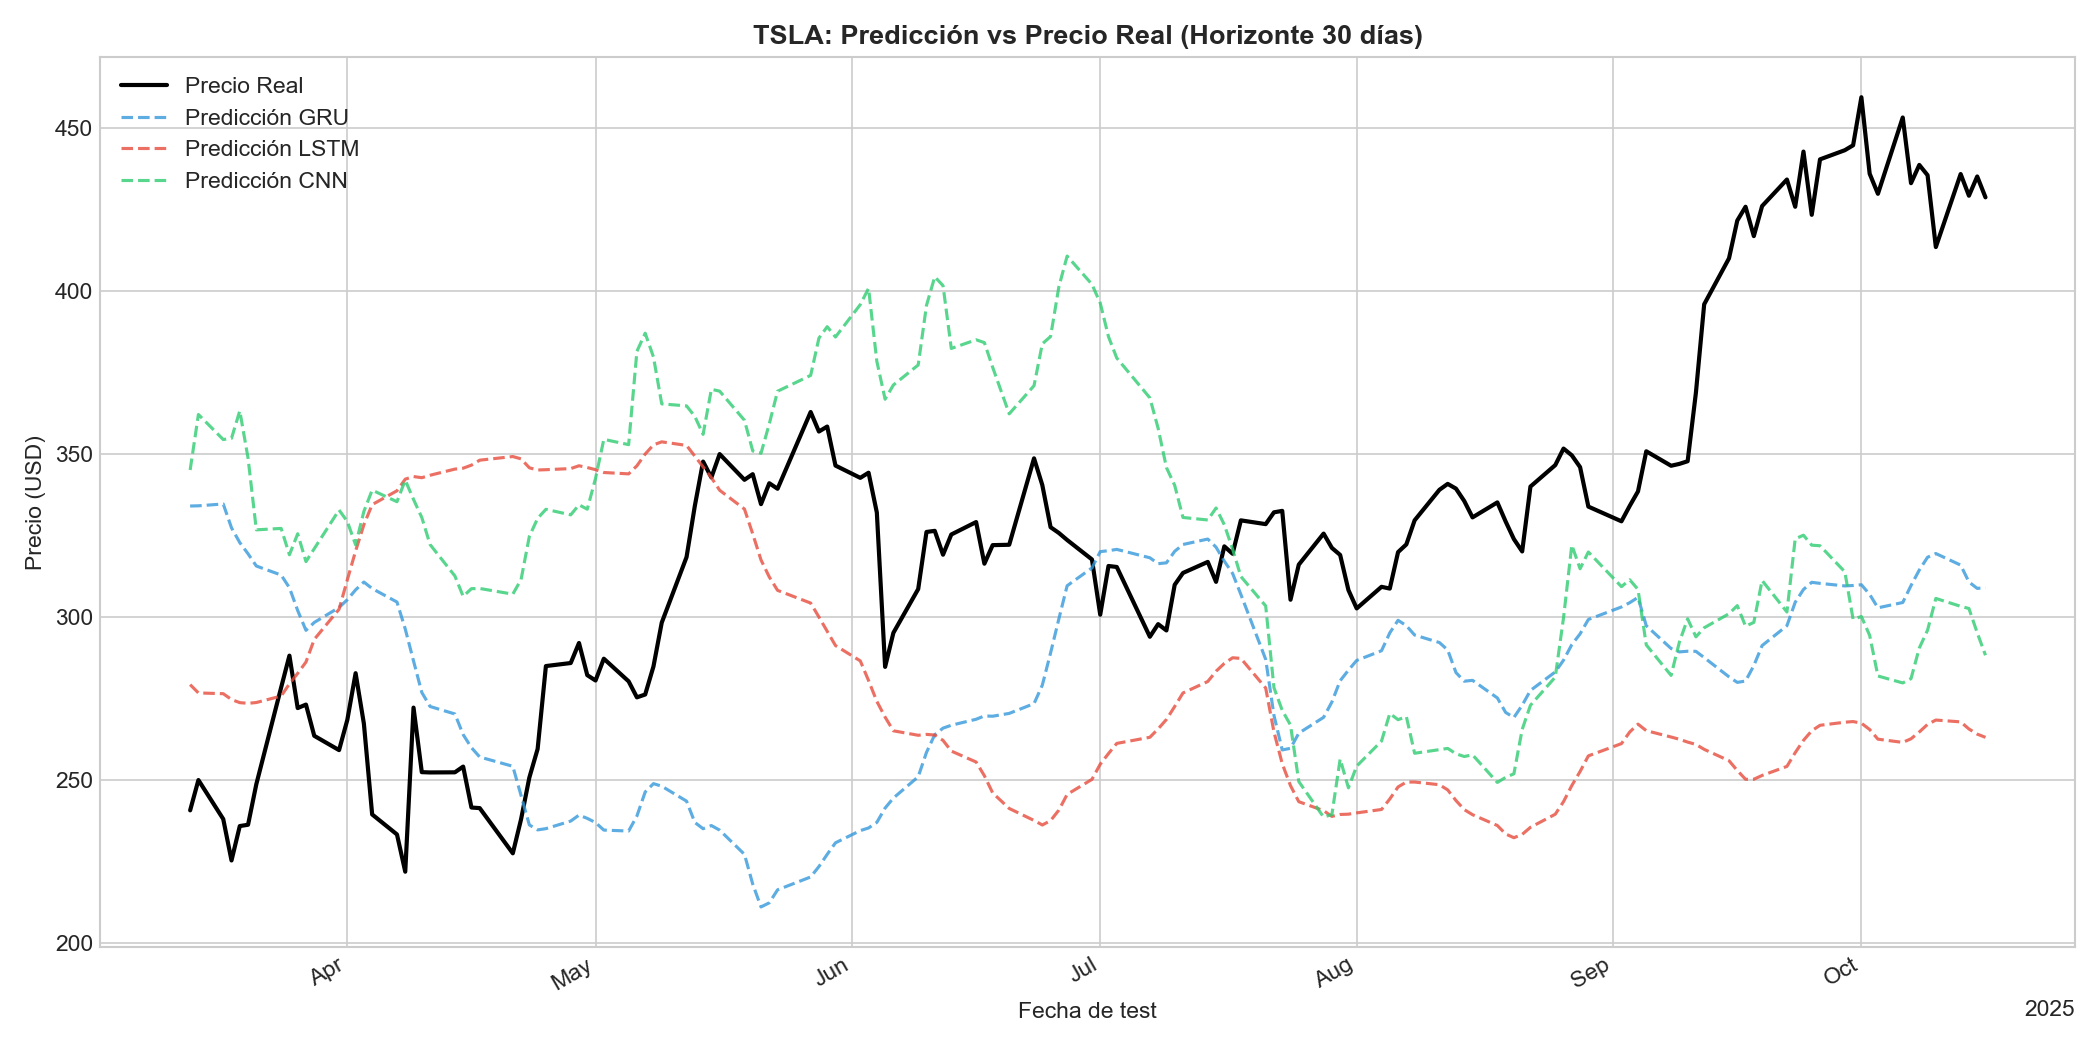
\includegraphics[width=0.95\textwidth]{Imagenes/pred_vs_actual_TSLA_h30.png}
\caption{TSLA: Predicción vs Real (30 días). Con horizonte de un mes, las predicciones capturan la tendencia general pero pierden precisión en los movimientos intermedios. Los cambios de régimen (por ejemplo, tras earnings o noticias de Elon Musk) son especialmente difíciles de anticipar.}
\label{fig:pred_tsla_h30}
\end{figure}

En conjunto, Tesla presenta una evolución más estable que Bitcoin en horizontes cortos en estas gráficas, pero un buen ajuste visual no implica necesariamente mejor MAPE: en la comparación global a 7 días, los baselines siguen siendo los modelos con menor error. Además, aunque el estudio de ablación sugiere una mejora ligera al incluir sentimiento en TSLA, el efecto no es estadísticamente significativo.

\clearpage
\subsection{Nvidia}

\begin{figure}[H]
\centering
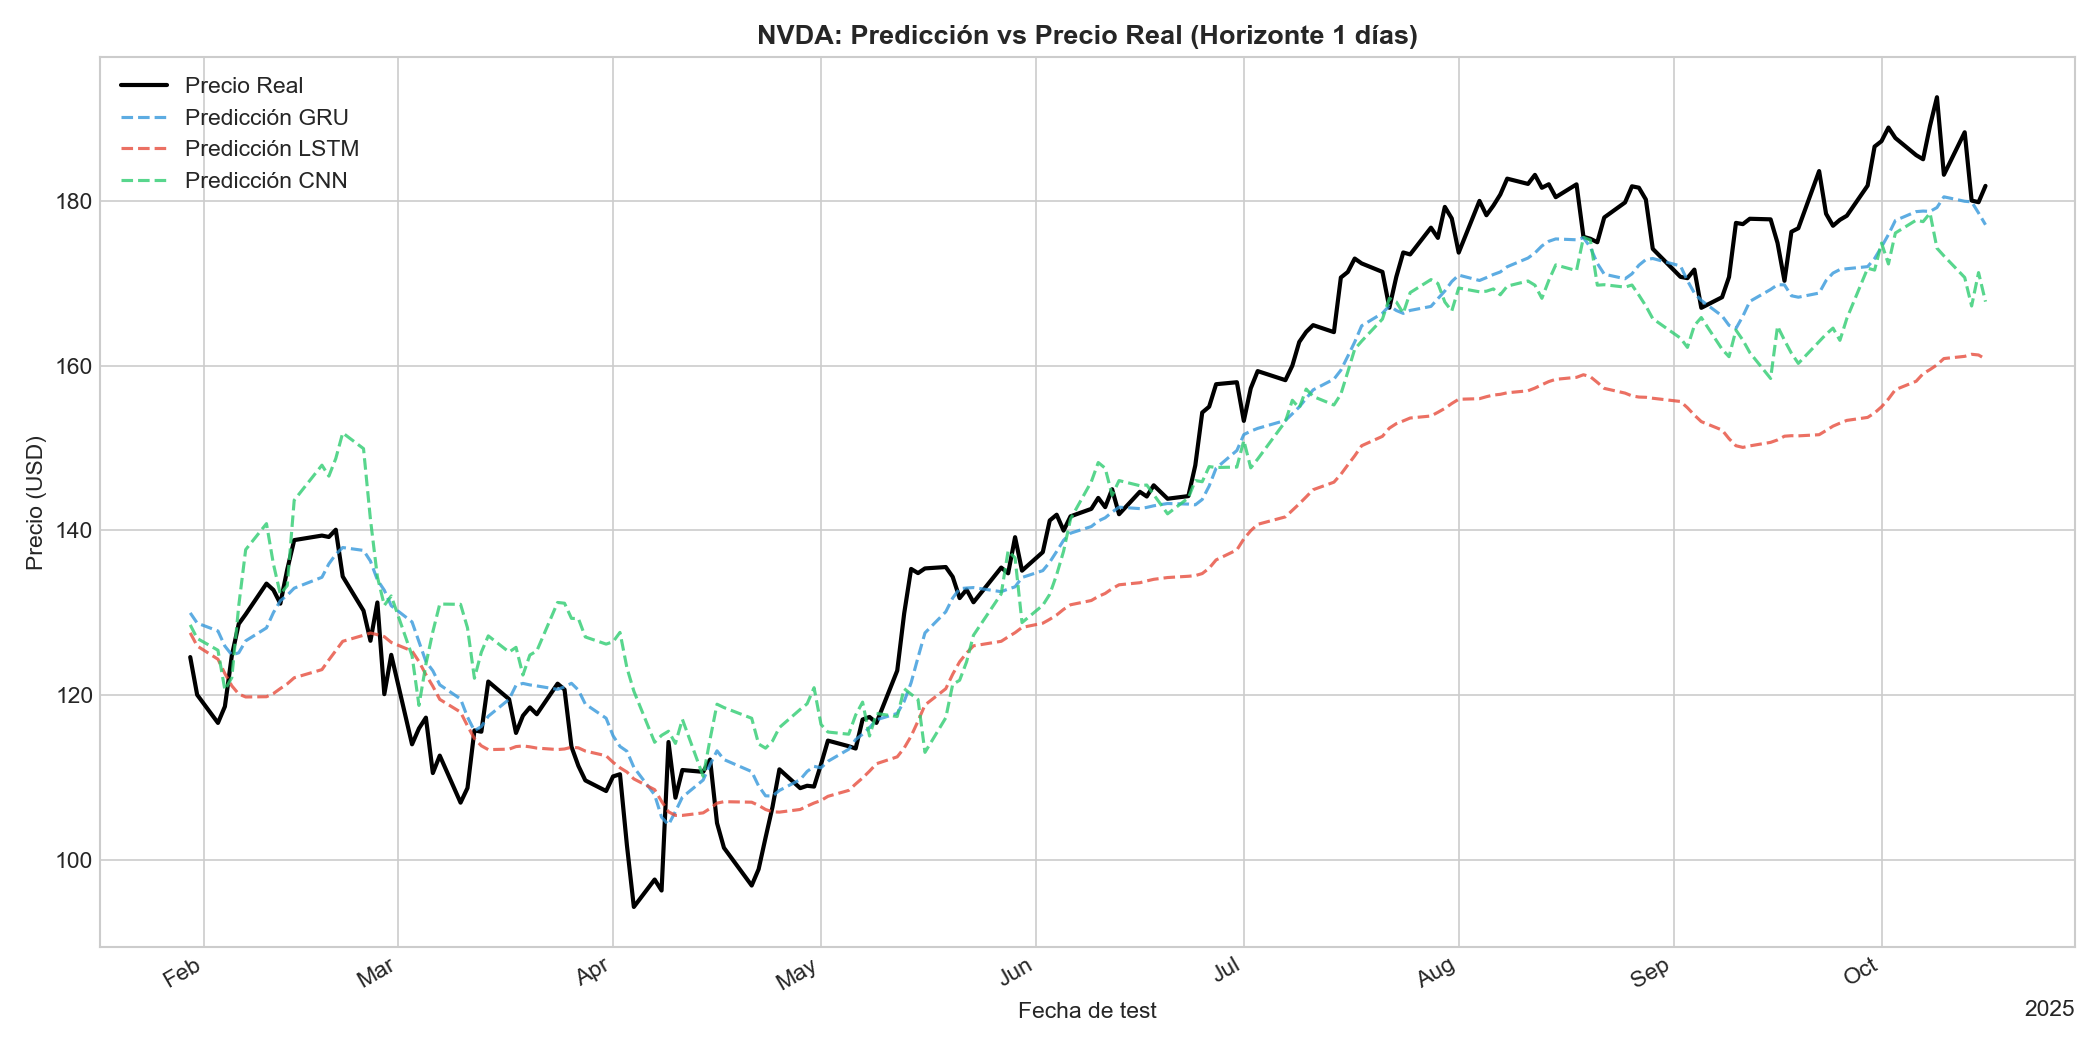
\includegraphics[width=0.95\textwidth]{Imagenes/pred_vs_actual_NVDA_h1.png}
\caption{NVDA: Predicción vs Real (1 día). Nvidia muestra un seguimiento cercano de la tendencia a corto plazo. Las oscilaciones diarias están bien capturadas, aunque con el típico retardo de los modelos basados en ventanas históricas.}
\label{fig:pred_nvda_h1}
\end{figure}

\begin{figure}[H]
\centering
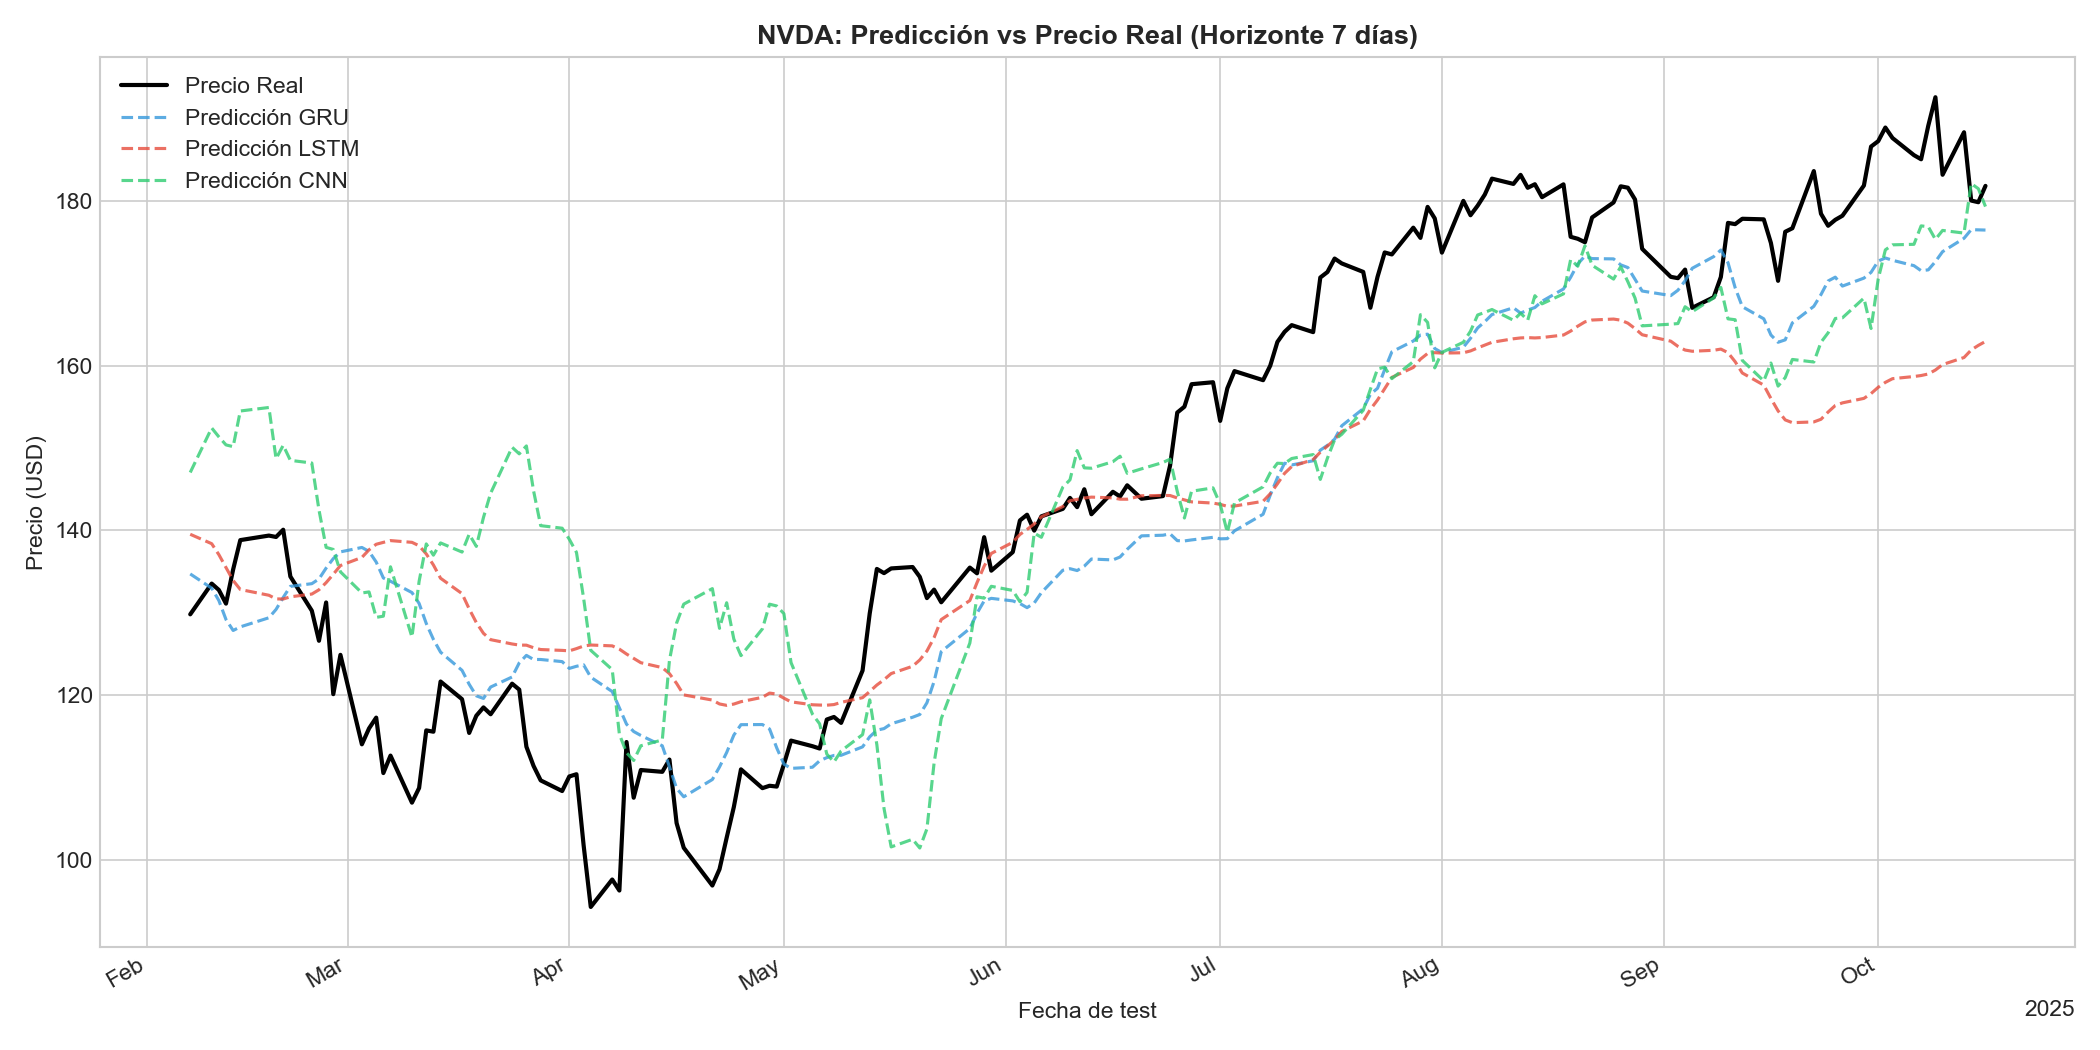
\includegraphics[width=0.95\textwidth]{Imagenes/pred_vs_actual_NVDA_h7.png}
\caption{NVDA: Predicción vs Real (7 días). A una semana, el modelo mantiene la dirección general pero pierde precisión en los puntos de inflexión. Los periodos de alta volatilidad ---especialmente durante noticias sobre IA--- presentan mayor error.}
\label{fig:pred_nvda_h7}
\end{figure}

\begin{figure}[H]
\centering
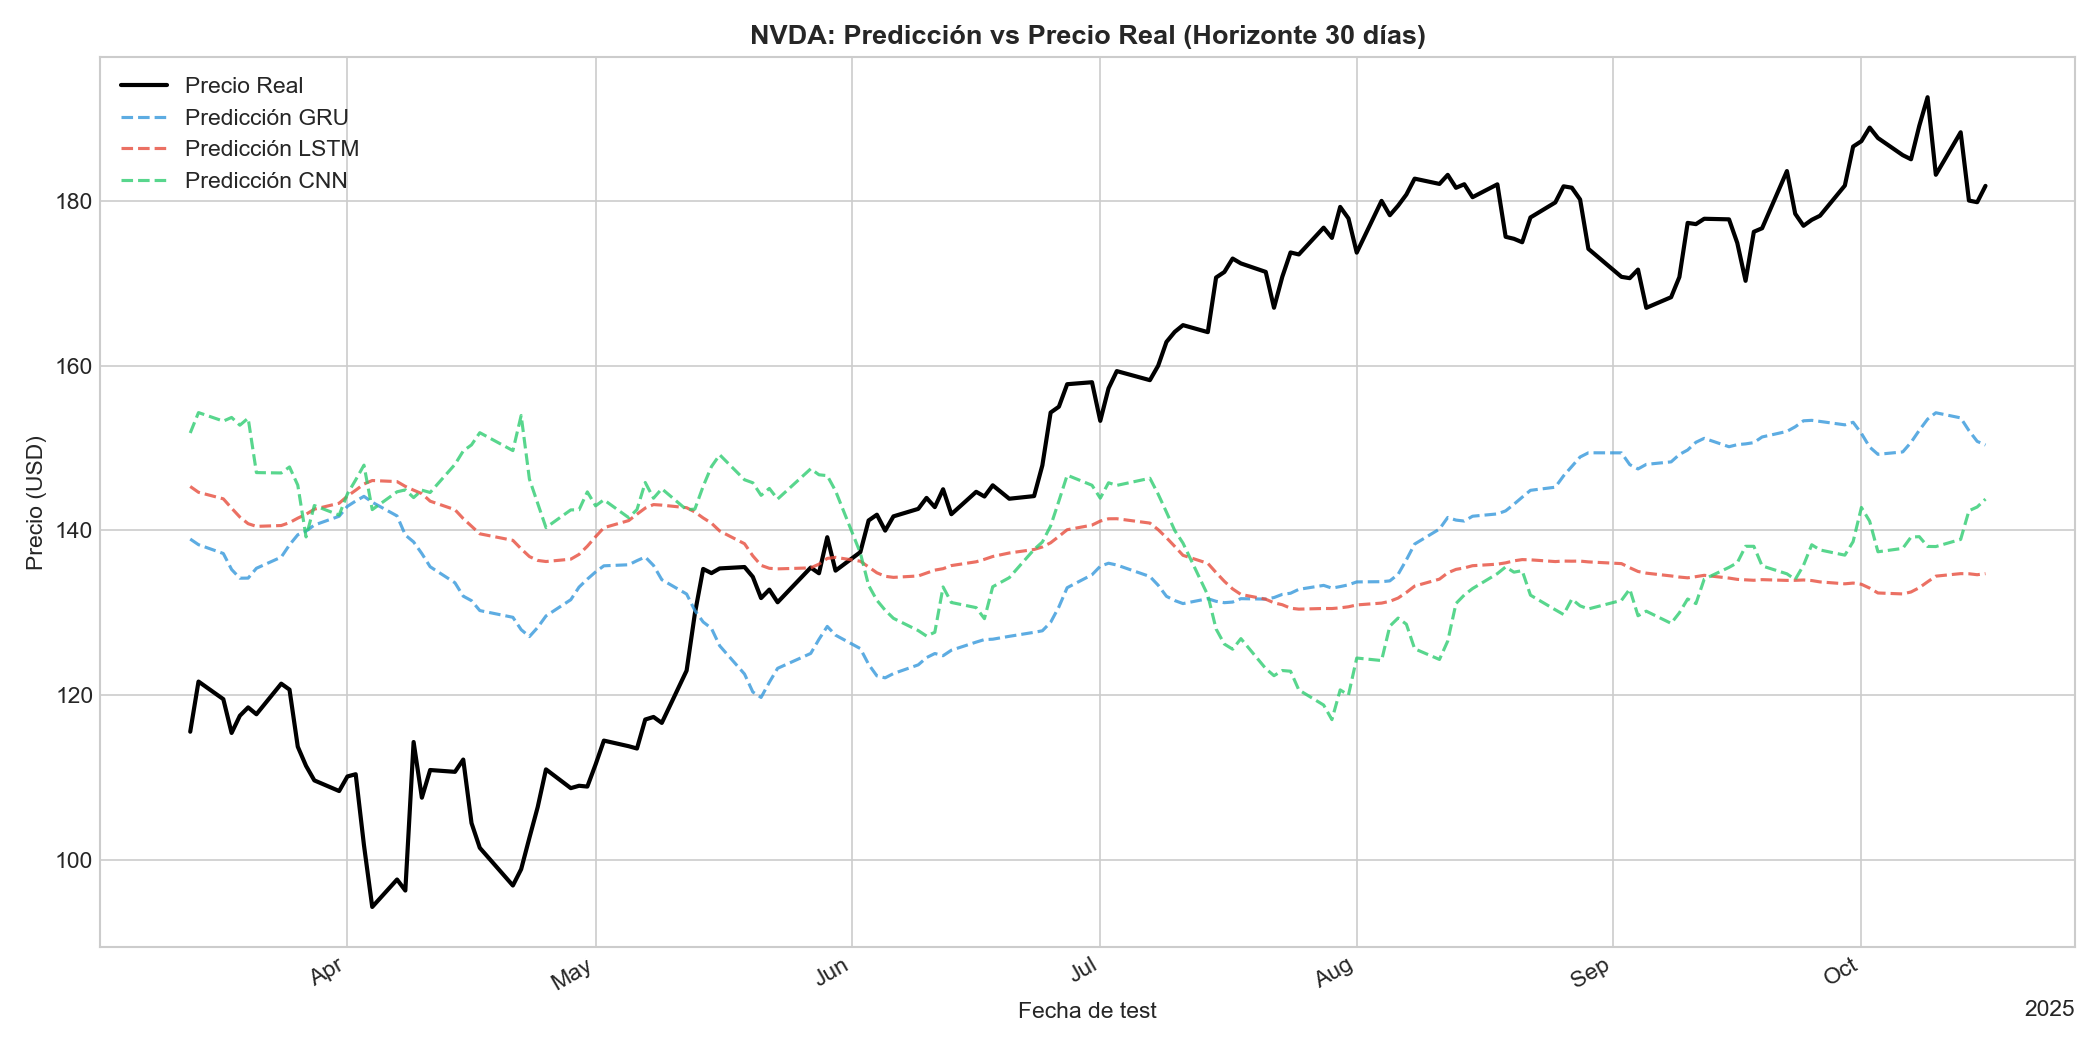
\includegraphics[width=0.95\textwidth]{Imagenes/pred_vs_actual_NVDA_h30.png}
\caption{NVDA: Predicción vs Real (30 días). Con horizonte mensual, la predicción captura movimientos de medio plazo pero falla en anticipar cambios de ritmo. La fuerte tendencia alcista del periodo analizado ayuda a que las predicciones sean razonables en términos de dirección.}
\label{fig:pred_nvda_h30}
\end{figure}

En Nvidia, las curvas muestran un seguimiento razonable de la tendencia, aunque con errores notables en los cambios de ritmo. Al ser el activo más vinculado al boom de la inteligencia artificial, su precio está fuertemente influenciado por noticias y expectativas del sector, lo que genera cambios de régimen difíciles de capturar. La lectura general es similar a la de los otros activos: existe estructura temporal aprovechable, pero la volatilidad y los eventos externos limitan la capacidad predictiva del modelo.

%% ============================================================
%% RESUMEN VISUAL
%% ============================================================

\clearpage
\section{Resumen visual}

Esta sección consolida los hallazgos principales mediante visualizaciones de síntesis. Aunque no añaden resultados nuevos, estas figuras facilitan la comparación de patrones y la comprensión global de los experimentos realizados.

\begin{figure}[H]
\centering
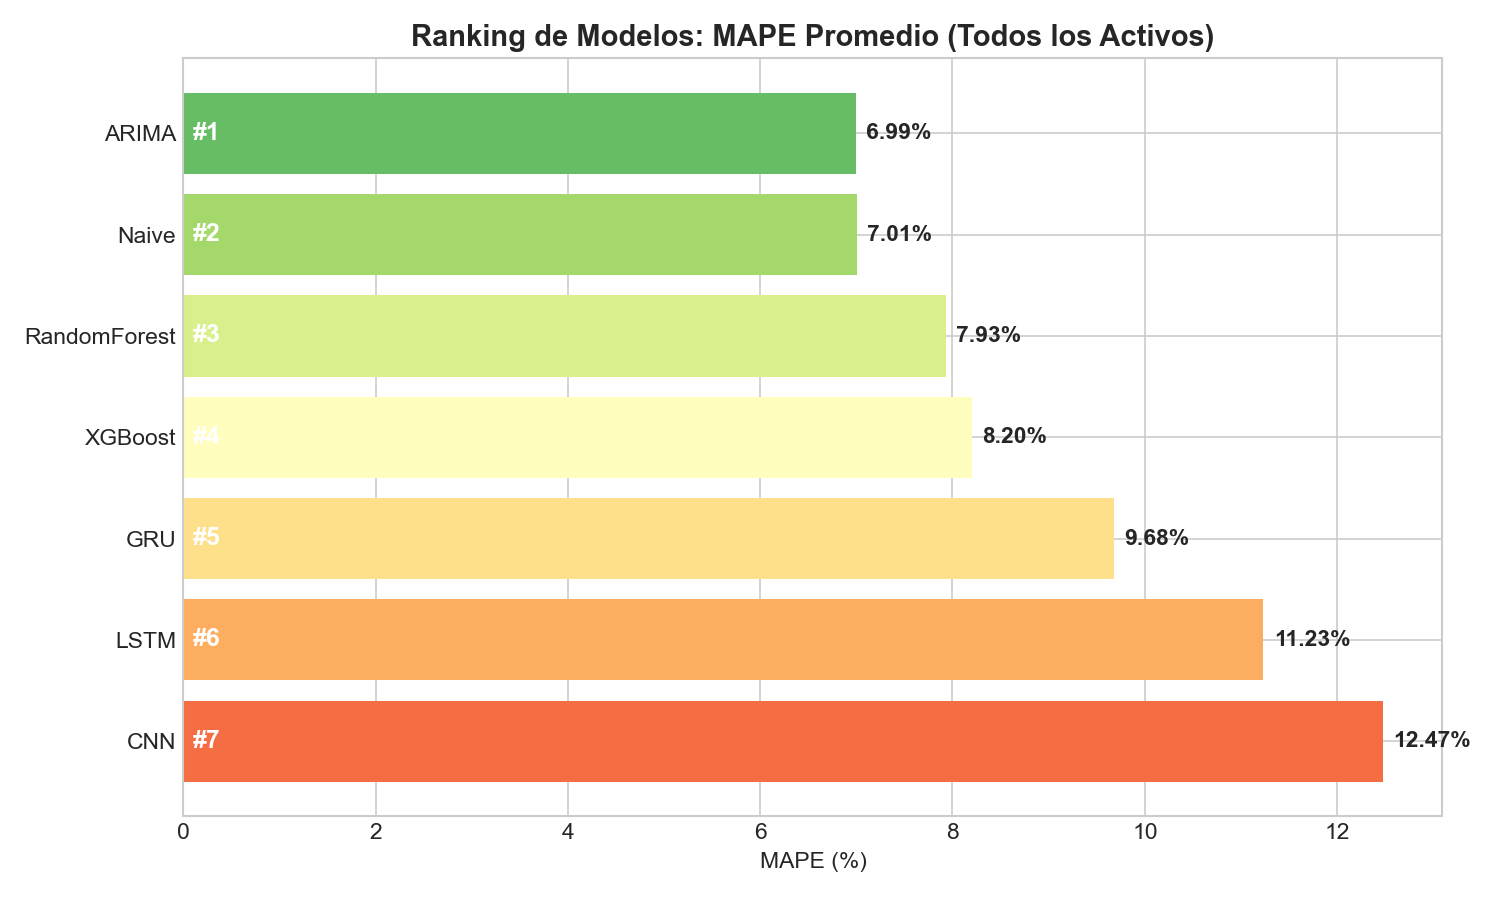
\includegraphics[width=0.90\textwidth]{Imagenes/summary_model_ranking.png}
\caption{Ranking global de modelos.}
\label{fig:summary_ranking}
\end{figure}

La Figura~\ref{fig:summary_ranking} presenta el ranking consolidado de los siete modelos evaluados. Se observa que los baselines (Naive y ARIMA) lideran el rendimiento medio, con los modelos de árboles a cierta distancia; las arquitecturas de aprendizaje profundo quedan en la parte baja del ranking. Esta visualización permite identificar rápidamente qué familias de modelos se acercan a los baselines y cuáles no justifican su complejidad adicional en esta configuración experimental.

\begin{figure}[H]
\centering
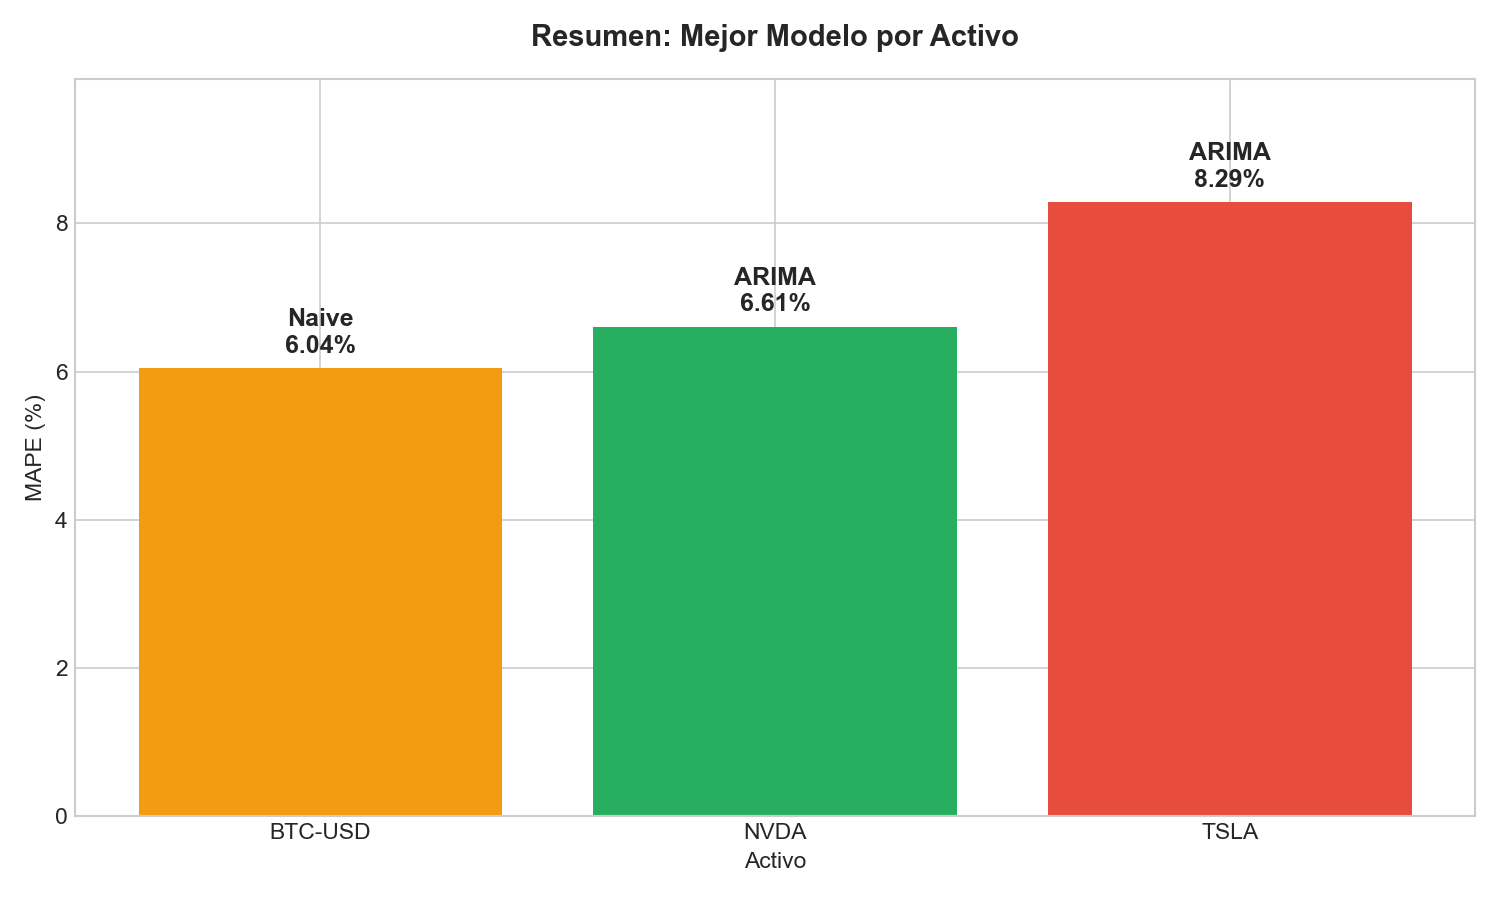
\includegraphics[width=0.85\textwidth]{Imagenes/summary_best_models.png}
\caption{Mejor modelo por activo.}
\label{fig:summary_best}
\end{figure}

La Figura~\ref{fig:summary_best} desglosa el mejor modelo para cada activo analizado. En este experimento, Naive es el mejor en BTC-USD, mientras que ARIMA lidera en TSLA y NVDA. Esta heterogeneidad refuerza la importancia de evaluar cada combinación modelo-activo de forma independiente.

\begin{figure}[H]
\centering
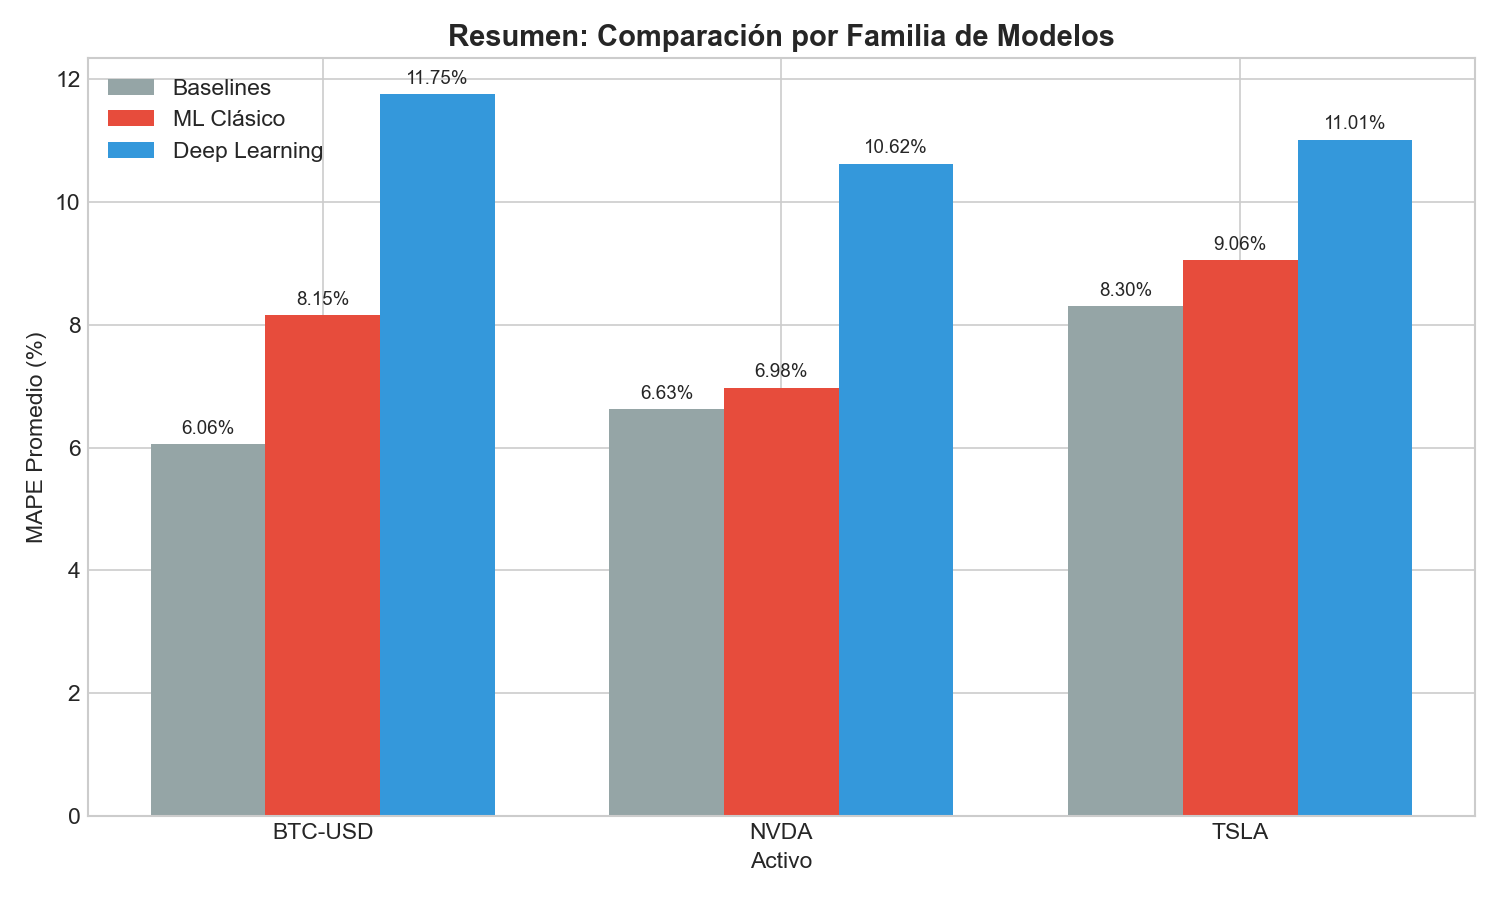
\includegraphics[width=0.90\textwidth]{Imagenes/summary_dl_vs_baselines.png}
\caption{Deep Learning vs Baselines.}
\label{fig:summary_dl_baselines}
\end{figure}

La Figura~\ref{fig:summary_dl_baselines} compara directamente los modelos de deep learning contra los baselines (Naive y ARIMA). Esta comparación es fundamental para responder a la pregunta de si la complejidad del deep learning aporta valor real. En estos resultados, los modelos DL no superan a los baselines en ninguno de los activos y presentan errores sustancialmente mayores, lo que sugiere que, con esta configuración, el valor añadido del deep learning no se materializa.

\begin{figure}[H]
\centering
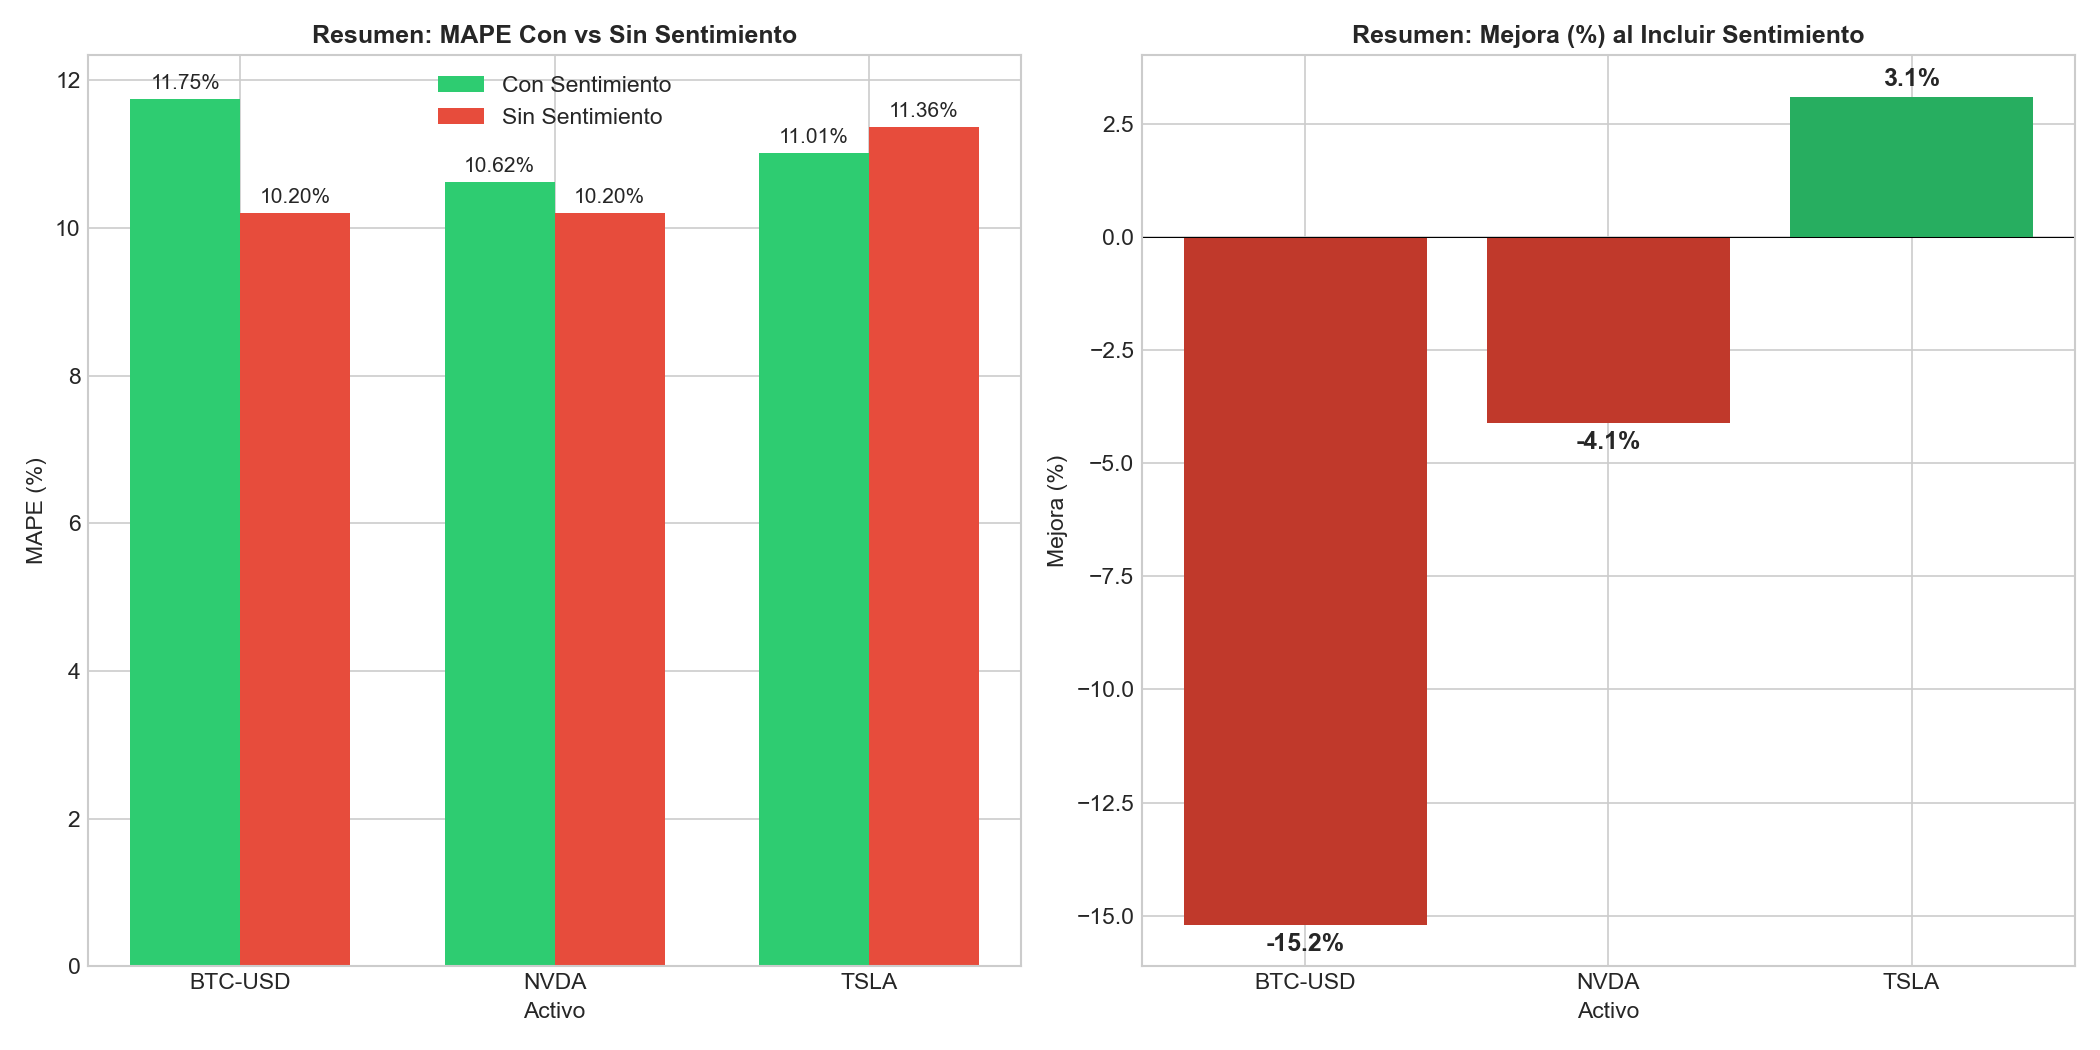
\includegraphics[width=0.95\textwidth]{Imagenes/summary_sentiment_impact.png}
\caption{Impacto del sentimiento.}
\label{fig:summary_sentiment}
\end{figure}

La Figura~\ref{fig:summary_sentiment} resume el impacto del sentimiento en las predicciones. El gráfico muestra que el efecto del sentimiento es heterogéneo: en Tesla tiende a mejorar ligeramente las predicciones, en Bitcoin tiende a perjudicar y en Nvidia solo LSTM se beneficia de forma leve. Esta visualización sintetiza el hallazgo principal del estudio de ablación: el sentimiento no es una mejora universal, sino que su utilidad depende de la combinación específica de modelo y activo.

\begin{figure}[H]
\centering
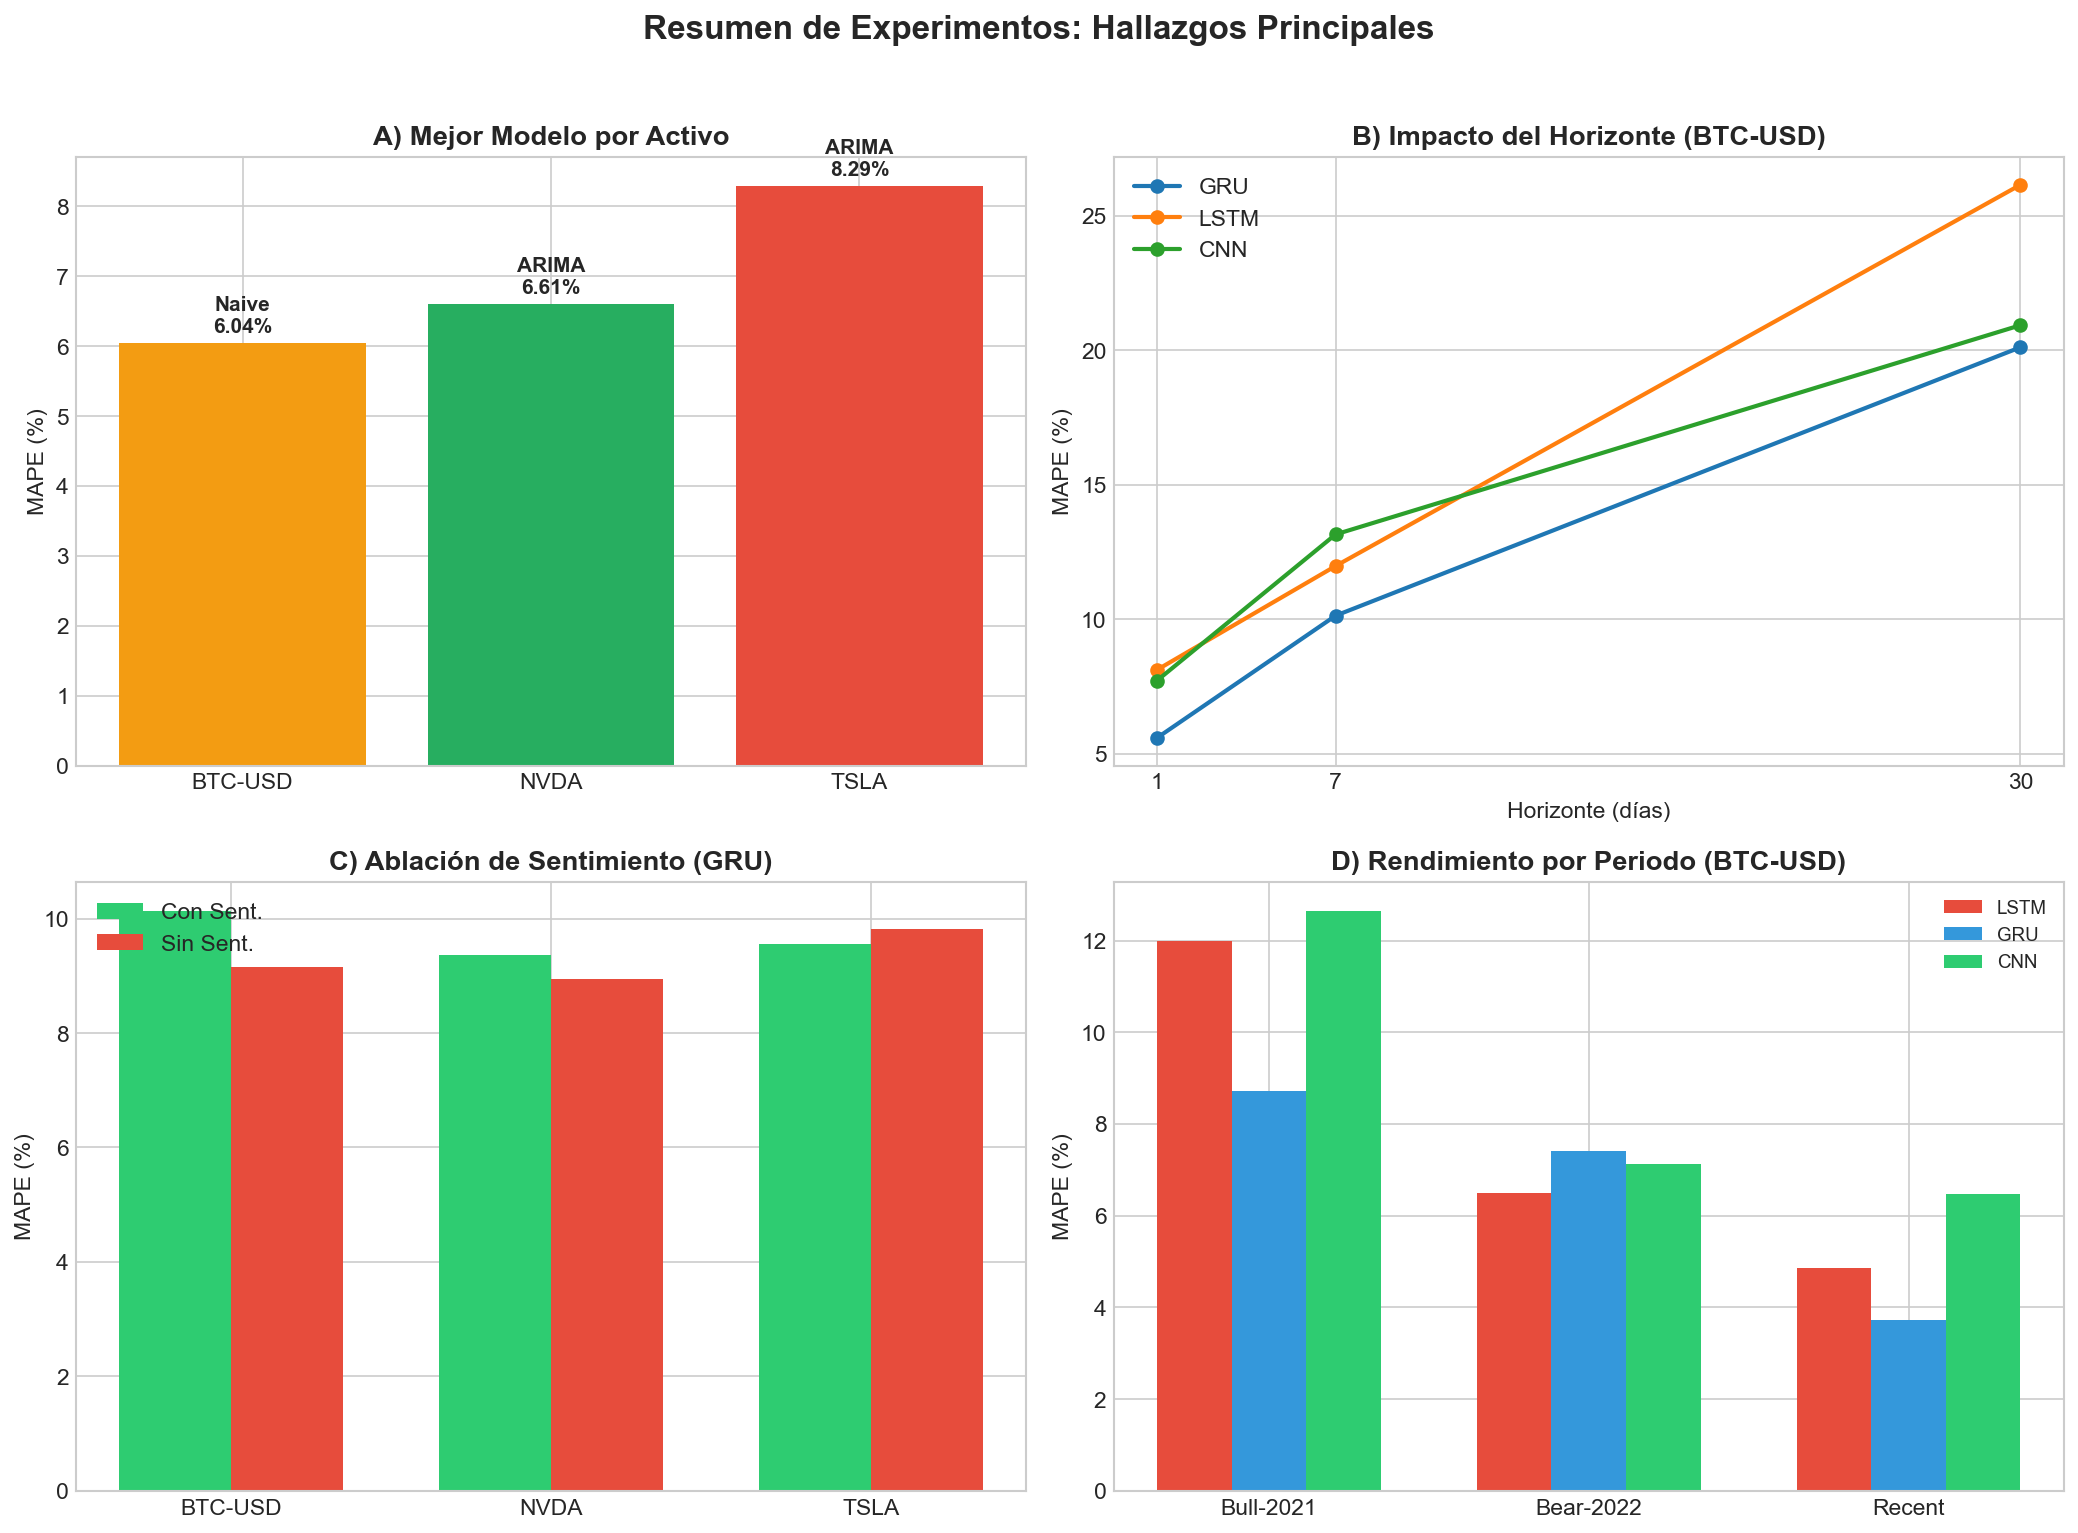
\includegraphics[width=0.95\textwidth]{Imagenes/summary_all_experiments.png}
\caption{Panel resumen de los cuatro experimentos.}
\label{fig:summary_all}
\end{figure}

Finalmente, la Figura~\ref{fig:summary_all} ofrece un panel que junta los cuatro experimentos (A: modelos, B: horizonte, C: ablación, D: periodos). Es la vista de pájaro del trabajo entero y ayuda a cruzar patrones que viendo cada experimento por separado podrían pasar desapercibidos.

\section{Lecciones extraídas de los datos}

Tras las figuras y tablas presentadas, estas son las conclusiones que los datos respaldan con cierta solidez:

\textbf{Los baselines dominan el MAPE.} ARIMA obtiene el mejor MAPE medio y Naive queda muy cerca; por activo, Naive lidera en BTC-USD y ARIMA en TSLA/NVDA. En esta configuración experimental, los modelos más complejos no mejoran esos baselines.

\textbf{CNN es el peor; los árboles no son competitivos.} CNN es sistemáticamente el modelo con mayor error. Random Forest y XGBoost quedan por detrás de Naive/ARIMA en los tres activos y, en BTC-USD, el test de Diebold-Mariano detecta empeoramiento significativo frente a Naive.

\textbf{GRU domina todos los horizontes en BTC.} A 1, 7 y 30 días mantiene el menor MAPE; LSTM queda por detrás y CNN se degrada al alargar el horizonte.

\textbf{La direccionalidad no muestra una ventaja robusta.} La precisión direccional se mueve típicamente en rangos cercanos al azar (aprox.\ 27--57\% según activo y modelo). Además, el baseline Naive genera una predicción ``plana'' y por eso su F1 direccional es 0, lo que ilustra que DA debe interpretarse junto con F1/MCC y el balance de clases.

\textbf{El sentimiento tiene un efecto pequeño y heterogéneo.} Mejora Tesla en los tres modelos y en NVDA solo con LSTM; empeora Bitcoin en los tres modelos y empeora también NVDA en CNN/GRU. En MAPE y DA/F1 no hay diferencias significativas según Wilcoxon (solo aparece un caso aislado en MCC).

\textbf{El rendimiento cambia por periodo, sin una regla simple.} En BTC-USD, GRU obtiene el mejor MAPE en el periodo reciente (3.71\%) y el peor en Bull-2021 (8.71\%). LSTM y CNN muestran una tendencia similar, pero el ranking entre ellos varía según el régimen: LSTM destaca en Bear-2022 y GRU en Bull-2021 y el periodo reciente. Conviene replicar con más particiones para confirmar estos patrones.

%% ============================================================
%% DISCUSIÓN CRÍTICA
%% ============================================================

\section{Discusión crítica: lo que los números no dicen}

Las tablas y gráficas presentan los datos de forma clara, pero conviene no sobreinterpretar un MAPE aparentemente bajo o unas curvas que parecen seguir la serie real. Un error bajo no significa utilidad práctica, y unas predicciones que ``parecen'' buenas visualmente pueden no aportar valor operativo si no superan tests estadísticos. En esta sección se ofrece una interpretación prudente de lo que los resultados sustentan y de sus limitaciones.

\subsection{Por qué los baselines dominan aquí}

En este esquema, Naive y ARIMA dominan de forma clara en MAPE en los tres activos. Una lectura plausible es que, para precios diarios y horizontes cortos, el cierre se comporta de forma cercana a un paseo aleatorio: la persistencia (``mañana parecido a hoy'') es muy difícil de batir. Cuando las señales adicionales (indicadores técnicos + sentimiento agregado) no aportan una ventaja estable, los modelos más complejos tienden a aprender ruido y a generalizar peor. El test de Diebold-Mariano refuerza esta lectura: no aparecen mejoras significativas frente a Naive y sí aparecen varios empeoramientos significativos.

\subsection{Interpretación realista del error}

Un MAPE de un solo dígito puede parecer reducido, pero conviene traducirlo a magnitudes absolutas para obtener una referencia de orden de magnitud.

\begin{itemize}
    \item BTC-USD: el mejor MAPE es $\sim$6\% y el precio medio del periodo ronda los 53.000 USD, así que el error medio está en torno a 3.200 USD.
    \item TSLA: el mejor MAPE es $\sim$8,3\% con precio medio cercano a 260 USD, lo que implica un error medio de unos 21 USD.
    \item NVDA: el mejor MAPE es $\sim$6,6\% con precio medio alrededor de 62 USD, lo que deja un error medio en torno a 4 USD.
\end{itemize}

Esto importa porque fija el orden de magnitud: si una estrategia no puede absorber errores de ese tamaño (más comisiones y spreads), la predicción deja de ser útil aunque el porcentaje parezca bajo.

Si quisiéramos usar estas predicciones para trading, tendríamos que considerar:

\textbf{Costes de transacción.} Entre spreads, comisiones y slippage, cada operación tiene un coste. Si el beneficio esperado es menor que el coste, la estrategia pierde dinero.

\textbf{Gestión del riesgo.} Un error medio del 5\% implica una distribución con valores más altos en determinados episodios (por ejemplo, 8\% o 12\%). La exposición y el tamaño de posición deberían ser coherentes con esa variabilidad.

\textbf{Frecuencia de operación.} Predicciones a 7 días implican pocas operaciones al año. Los beneficios tendrían que ser sustanciales para compensar el capital inmovilizado.

No se ha realizado un backtesting riguroso con costes reales; no obstante, es razonable anticipar que un MAPE moderado puede ser insuficiente para generar beneficios consistentes una vez incorporados costes de transacción y fricciones. Además, incluso cuando una curva de predicción aparenta seguir la serie real, ello no implica ventaja operativa ni superioridad estadística frente a un baseline.

\subsection{Precisión direccional: la métrica que importa}

En contextos de decisión, además del error absoluto, resulta relevante anticipar si el precio subirá o bajará. Para ello se utiliza la \textbf{precisión direccional}, definida como el porcentaje de veces que el modelo acierta la dirección del movimiento.

Se calcularon estas métricas para todos los modelos. La Tabla~\ref{tab:directional_accuracy} resume acierto direccional, F1 y MCC.

\begin{table}[H]
\centering
\caption{Métricas direccionales por modelo y activo}
\label{tab:directional_accuracy}
\begin{tabular}{l|ccc|c}
\hline
\textbf{Modelo/Metrica} & \textbf{BTC-USD} & \textbf{TSLA} & \textbf{NVDA} & \textbf{Media} \\
\hline
Naive - DA (\%) & 50.28 & 53.89 & 26.94 & 43.70 \\
Naive - F1 dir. (\%) & 0.00 & 0.00 & 0.00 & 0.00 \\
Naive - MCC & 0.00 & 0.00 & 0.00 & 0.00 \\
ARIMA - DA (\%) & 46.39 & 50.00 & 56.94 & 51.11 \\
ARIMA - F1 dir. (\%) & 41.97 & 44.91 & 64.46 & 50.45 \\
ARIMA - MCC & -0.16 & 0.06 & 0.02 & -0.03 \\
RandomForest - DA (\%) & 46.39 & 47.78 & 54.44 & 49.54 \\
RandomForest - F1 dir. (\%) & 39.40 & 36.59 & 53.29 & 43.09 \\
RandomForest - MCC & -0.00 & 0.02 & 0.13 & 0.05 \\
XGBoost - DA (\%) & 47.22 & 48.89 & 53.06 & 49.72 \\
XGBoost - F1 dir. (\%) & 42.23 & 32.30 & 51.04 & 41.86 \\
XGBoost - MCC & 0.05 & -0.06 & 0.16 & 0.05 \\
CNN - DA (\%) & 45.56 & 47.22 & 39.72 & 44.17 \\
CNN - F1 dir. (\%) & 34.39 & 43.45 & 32.55 & 36.80 \\
CNN - MCC & 0.07 & 0.09 & -0.04 & 0.04 \\
LSTM - DA (\%) & 46.39 & 55.83 & 39.17 & 47.13 \\
LSTM - F1 dir. (\%) & 42.34 & 46.43 & 36.68 & 41.82 \\
LSTM - MCC & 0.05 & 0.17 & 0.08 & 0.10 \\
GRU - DA (\%) & 46.94 & 55.56 & 43.33 & 48.61 \\
GRU - F1 dir. (\%) & 41.78 & 36.76 & 38.38 & 38.98 \\
GRU - MCC & 0.01 & 0.08 & 0.11 & 0.07 \\
\hline
\end{tabular}
\end{table}

Los resultados muestran heterogeneidad. La dirección se comporta de forma distinta a los errores absolutos: hay activos donde algunos modelos aciertan más la dirección aun sin ser los mejores en MAPE, y viceversa. Esto refuerza que las métricas direccionales son sensibles al periodo de test y al activo, y deben leerse con cautela. Por tanto, la selección del ``mejor modelo'' depende de la métrica objetivo.

En este protocolo se obtienen 360 predicciones en el test por activo. La mayoría de modelos se sitúan en torno al 50\% de precisión direccional y, aunque existen diferencias entre activos, no aparece una ventaja direccional grande y estable. Además, el baseline Naive produce un cambio predicho igual a 0 (predicción plana), por lo que su F1 direccional es 0; esto recuerda que la DA debe interpretarse junto con F1/MCC y el balance de clases.

Conviene matizar, sin embargo, que un acierto direccional elevado no implica necesariamente utilidad económica. Si los errores se concentran en jornadas con movimientos grandes, su impacto puede superar el de múltiples aciertos en jornadas con movimientos pequeños. Además, con ventanas de test relativamente cortas, estas proporciones pueden verse afectadas por variabilidad muestral. La Figura~\ref{fig:directional_accuracy} visualiza estos resultados.

\begin{figure}[H]
\centering
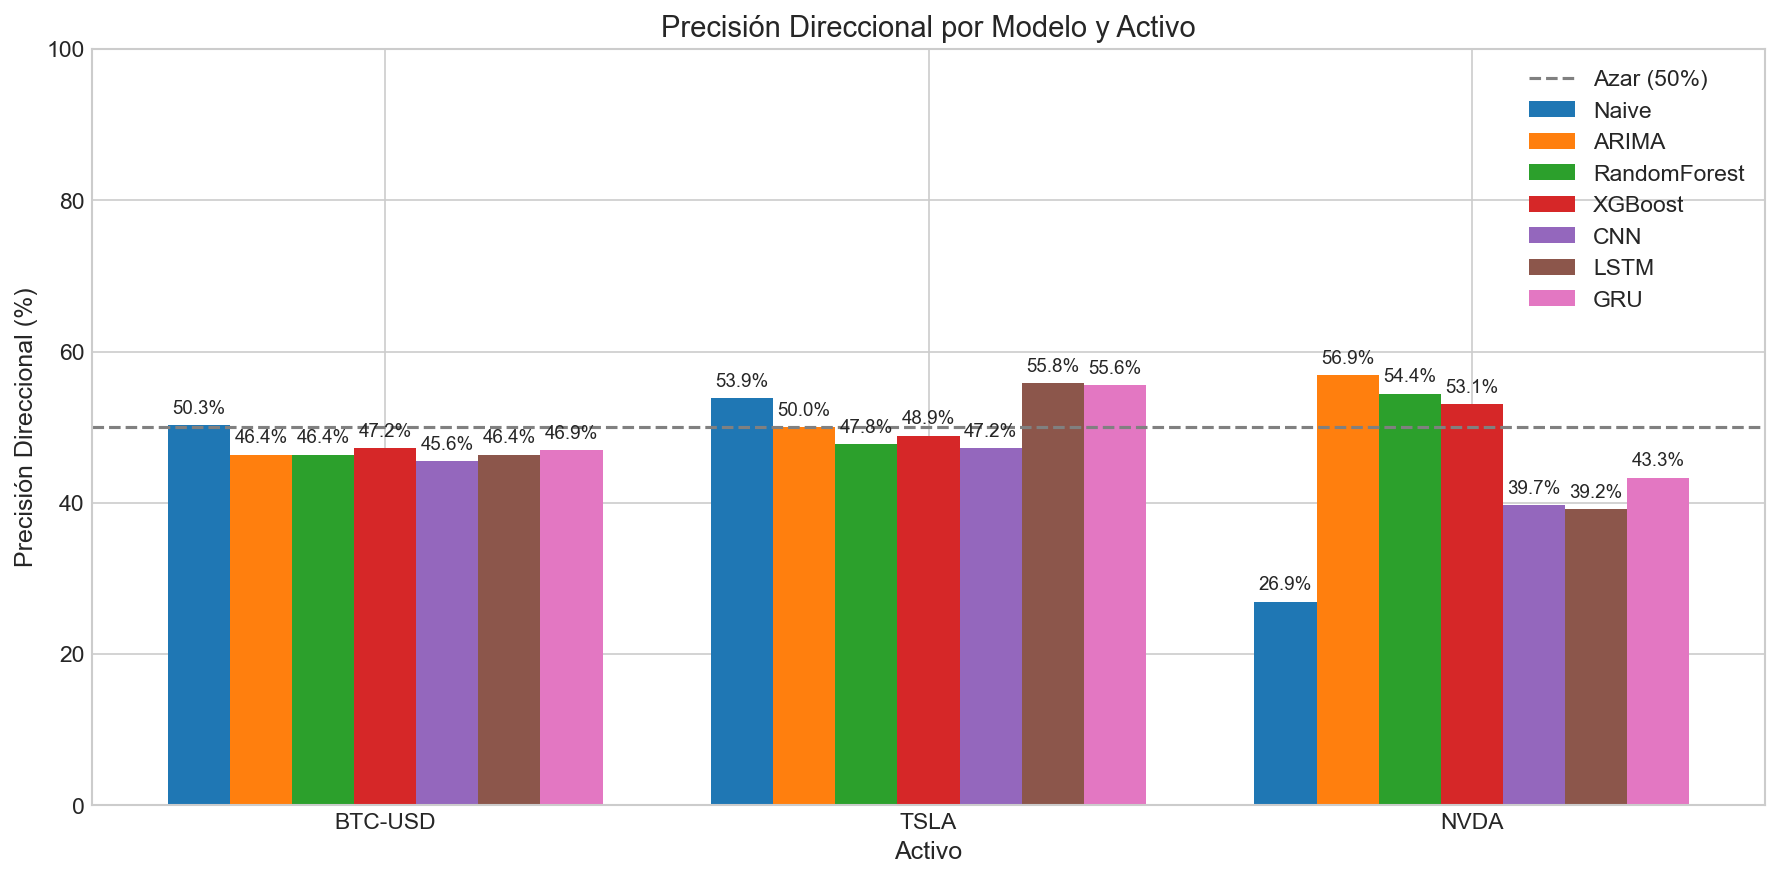
\includegraphics[width=0.95\textwidth]{Imagenes/directional_accuracy_comparison.png}
\caption{Precisión direccional por modelo y activo. La línea discontinua marca el 50\% (azar).}
\label{fig:directional_accuracy}
\end{figure}

\subsection{Significancia estadística de las diferencias}

La cuestión relevante es si un modelo mejora realmente a Naive o si la diferencia podría explicarse por ruido muestral. El \textbf{test de Diebold-Mariano}~\cite{diebold1995comparing} permite responder formalmente a esta pregunta comparando los errores de dos modelos. En este trabajo se ejecuta con horizonte 7, igual que el horizonte de predicción principal.

La Tabla~\ref{tab:diebold_mariano} muestra los resultados del test para cada activo y modelo comparado contra Naive.

\begin{table}[H]
\centering
\caption{Test de Diebold-Mariano: Naive vs cada modelo}
\label{tab:diebold_mariano}
\begin{tabular}{l|l|ccc}
\hline
\textbf{Activo} & \textbf{Modelo} & \textbf{Estadistico DM} & \textbf{p-value} & \textbf{Significativo?} \\
\hline
BTC-USD & ARIMA & -0.41 & 0.682 & No \\
BTC-USD & CNN & 3.52 & 0.000 & Si \\
BTC-USD & GRU & 2.63 & 0.009 & Si \\
BTC-USD & LSTM & 2.69 & 0.007 & Si \\
BTC-USD & RandomForest & 2.21 & 0.028 & Si \\
BTC-USD & XGBoost & 2.71 & 0.007 & Si \\
NVDA & ARIMA & -0.58 & 0.565 & No \\
NVDA & CNN & 2.81 & 0.005 & Si \\
NVDA & GRU & 2.48 & 0.014 & Si \\
NVDA & LSTM & 2.77 & 0.006 & Si \\
NVDA & RandomForest & -1.23 & 0.220 & No \\
NVDA & XGBoost & -0.69 & 0.489 & No \\
TSLA & ARIMA & 0.31 & 0.754 & No \\
TSLA & CNN & 2.75 & 0.006 & Si \\
TSLA & GRU & 1.50 & 0.135 & No \\
TSLA & LSTM & 1.63 & 0.103 & No \\
TSLA & RandomForest & 1.03 & 0.302 & No \\
TSLA & XGBoost & 0.93 & 0.351 & No \\
\hline
\end{tabular}
\end{table}

La Figura~\ref{fig:dm_pvalues} resume los p-values del test frente a Naive y permite apreciar que no aparecen mejoras robustas.

\begin{figure}[H]
\centering
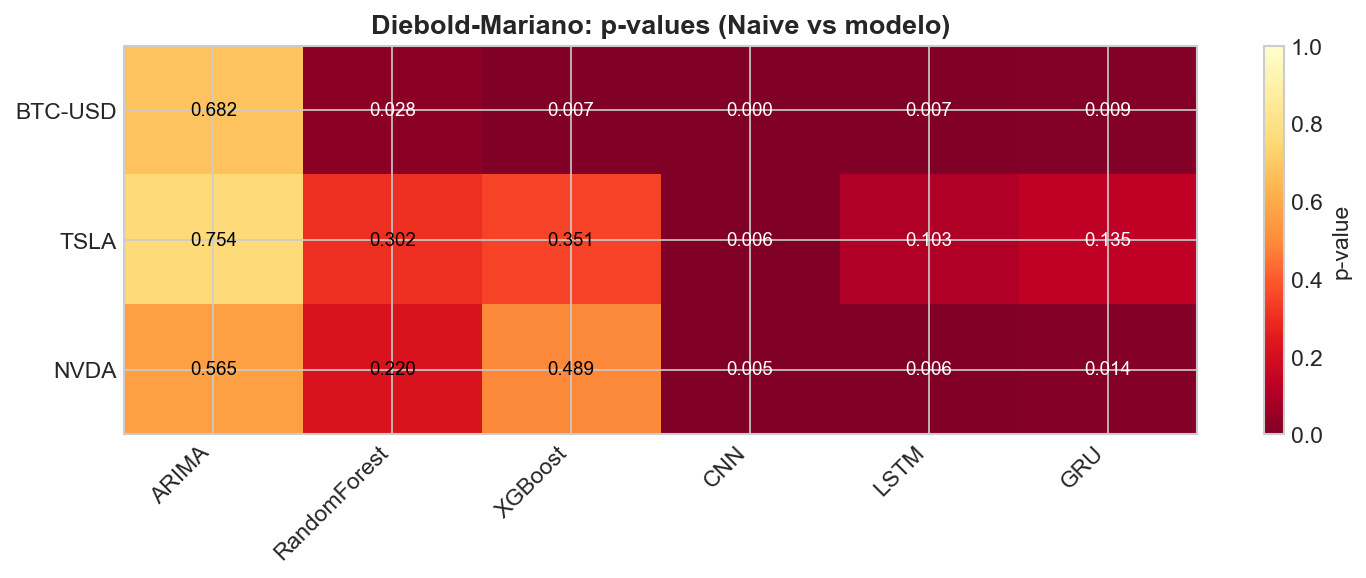
\includegraphics[width=0.90\textwidth]{Imagenes/diebold_mariano_pvalues_heatmap.png}
\caption{P-values del test de Diebold-Mariano (Naive vs cada modelo).}
\label{fig:dm_pvalues}
\end{figure}

Los resultados muestran dos hechos: (1) no hay evidencia de que ningún modelo mejore significativamente a Naive; y (2) sí aparecen empeoramientos significativos en varias comparaciones (especialmente CNN/LSTM/GRU en BTC-USD y NVDA, CNN en TSLA, y también Random Forest/XGBoost en BTC-USD). ARIMA, por su parte, no difiere significativamente de Naive.

\subsection{Limitación clave: eventos externos}

Una limitación estructural de este enfoque es que los modelos se entrenan con información observable en el histórico (precio, indicadores y sentimiento agregado). Sin embargo, eventos externos (anuncios corporativos, cambios regulatorios, noticias inesperadas) pueden provocar movimientos abruptos que no están reflejados de forma directa en las variables de entrada. En esos casos, el error aumenta para todos los modelos, independientemente de su complejidad.

Por tanto, lo máximo que puede esperarse de estos modelos es capturar la componente relativamente estable y repetible de la dinámica del precio. Esto ayuda a explicar por qué el rendimiento tiende a degradarse en fases de alta incertidumbre o cambios de régimen: cuando aumenta el peso de los shocks, la parte ``predecible'' se reduce.

\begin{figure}[H]
\centering
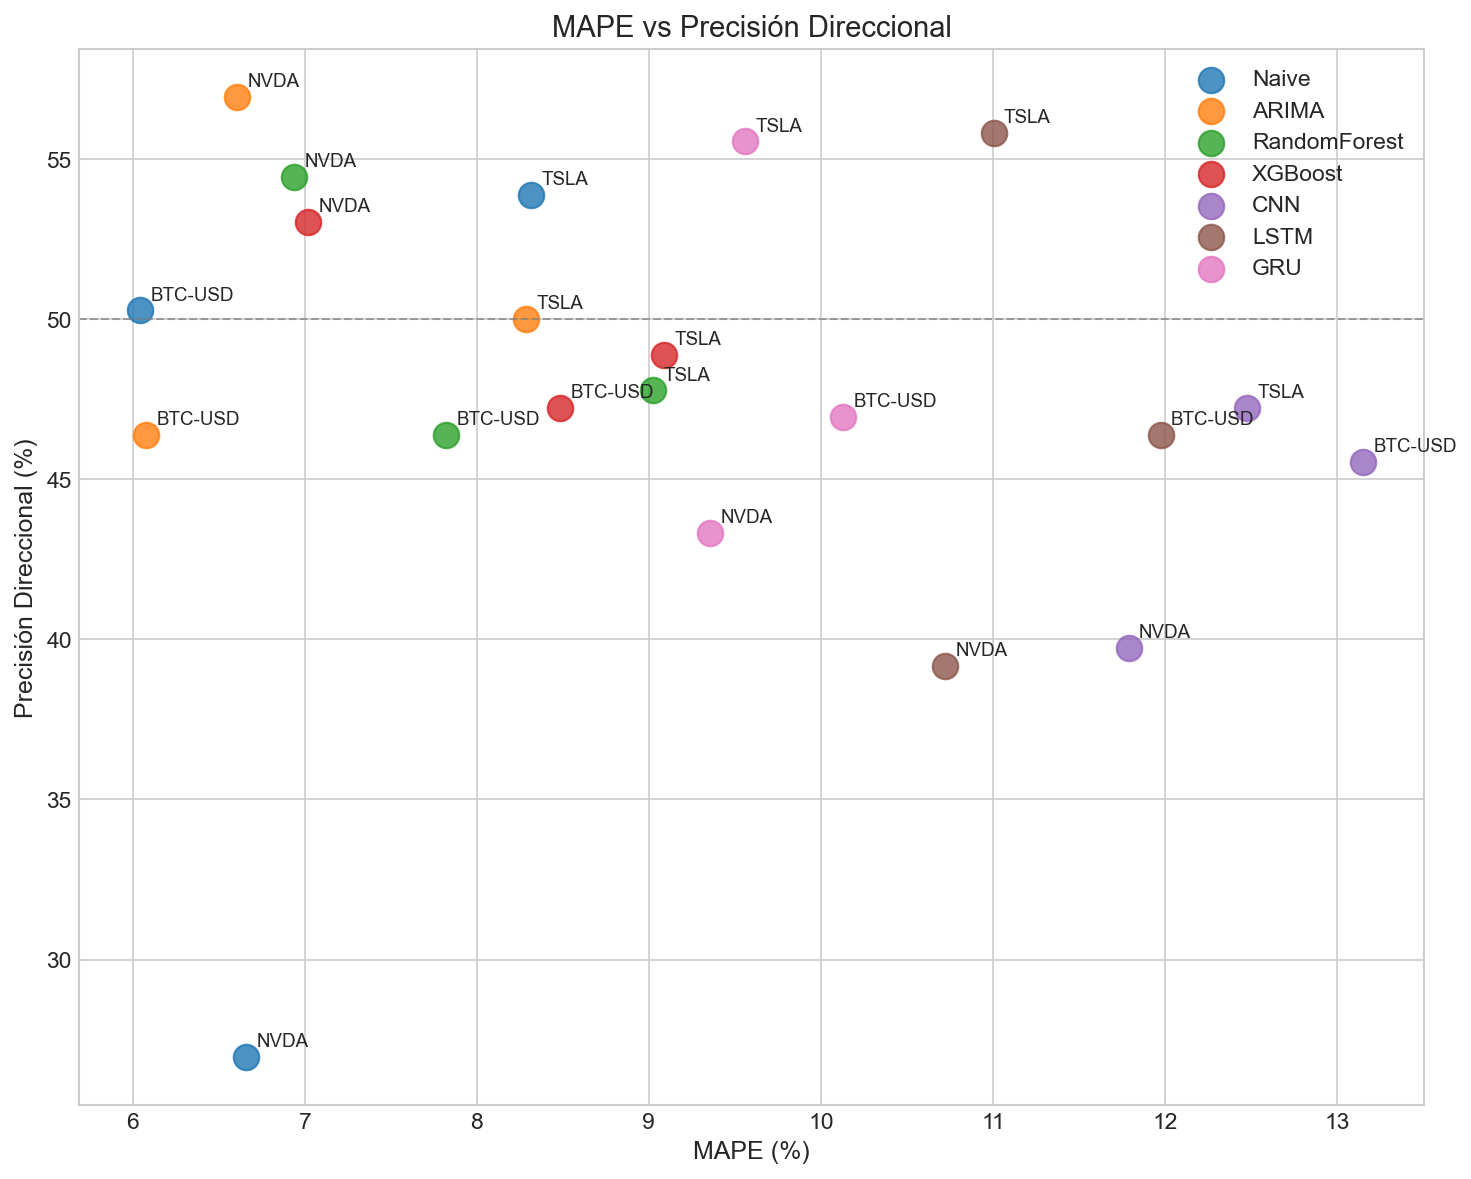
\includegraphics[width=0.90\textwidth]{Imagenes/mape_vs_directional_accuracy.png}
\caption{Relación entre MAPE y Precisión Direccional. Nótese que un MAPE bajo no siempre implica alta precisión direccional.}
\label{fig:mape_vs_da}
\end{figure}

La Figura~\ref{fig:mape_vs_da} muestra la relación entre MAPE y precisión direccional. Curiosamente, no hay una correlación perfecta: algunos modelos con MAPE similar tienen precisiones direccionales muy diferentes. Esto refuerza la idea de que ambas métricas capturan aspectos distintos del rendimiento predictivo.

\chapter{Conclusiones y trabajo futuro}
\label{ch:conclusion}

En este capítulo se recogen los hallazgos principales, se repasa hasta qué punto se han cumplido los objetivos y se apuntan direcciones de trabajo futuro.

\section{Resultados principales}

La pregunta central era si el sentimiento del mercado mejora las predicciones de precio. Con los datos y el protocolo empleados, la respuesta es que \textbf{no de forma clara}.

En términos de error (MAPE), los baselines simples siguen siendo difíciles de batir: \textbf{ARIMA} obtiene el mejor MAPE medio y \textbf{Naive} queda muy cerca; por activo, Naive lidera en BTC-USD y ARIMA en TSLA y NVDA. Random Forest y XGBoost no mejoran a esos baselines, y el test de Diebold-Mariano detecta \textbf{empeoramientos significativos} frente a Naive en BTC-USD (incluyendo RF/XGBoost) y en varios modelos DL (especialmente en BTC-USD y NVDA; en TSLA, CNN también empeora de forma significativa). Las arquitecturas de aprendizaje profundo (CNN, LSTM y GRU) presentan errores claramente superiores; dentro de la familia DL, GRU es la arquitectura más estable al variar el horizonte, pero en el experimento principal a 7 días sigue quedando lejos de los baselines.

Sobre el sentimiento, el estudio de ablación muestra un efecto pequeño y heterogéneo: en MAPE \textbf{mejora TSLA} en los tres modelos DL y mejora ligeramente NVDA en LSTM, pero \textbf{empeora BTC-USD} y empeora también NVDA en CNN/GRU. Sin embargo, el test de Wilcoxon no encuentra diferencias significativas en MAPE ni en DA/F1, y solo aparece un caso aislado en MCC; por tanto, estos cambios deben leerse como tendencias y no como evidencia concluyente.

La direccionalidad aporta una perspectiva distinta, pero los resultados siguen siendo modestos (valores cercanos al 50\% en muchas combinaciones) y sensibles al activo y al periodo. En resumen, este trabajo refuerza la importancia de comparar contra baselines y de acompañar los promedios con tests estadísticos antes de afirmar ventaja predictiva.

\section{Sobre los objetivos específicos}

Al inicio del trabajo se marcaron siete objetivos concretos. A continuación se evalúa el grado de cumplimiento de cada uno.

\textbf{Selección y descarga de activos.} Cumplido. Se seleccionaron tres activos con perfiles diferentes (BTC-USD, TSLA y NVDA) y se descargaron varios años de datos de precios. Para el sentimiento se utilizó GDELT y para precios Yahoo Finance.

\textbf{Preprocesamiento de datos.} Cumplido. El pipeline de preprocesado calcula indicadores técnicos, alinea el sentimiento y genera las variables objetivo para distintos horizontes. Está implementado como módulo reutilizable (ver Anexo~\ref{ch:codigo}).

\textbf{Incorporación del sentimiento.} Cumplido. La señal se extrae de GDELT con consultas específicas por activo (nombre y ticker) y se alinea por fecha sin usar información futura.

\textbf{Implementación de modelos.} Cumplido. Se implementaron siete modelos de tres familias distintas, desde baselines simples hasta redes recurrentes con dropout, en Python con librerías estándar.

\textbf{Definición del protocolo de evaluación.} Cumplido. Se utilizó validación walk-forward, doce iteraciones y métricas estándar (RMSE, MAE, MAPE), además de métricas direccionales, un test de Wilcoxon para la ablación y un test de Diebold-Mariano frente a Naive.

\textbf{Análisis de resultados.} Cumplido. Se generaron tablas y visualizaciones, un estudio de ablación y un análisis por periodo de mercado. El análisis es amplio, aunque con limitaciones.

\textbf{Conclusiones sobre el sentimiento.} Cumplido. La conclusión es matizada: el sentimiento muestra un efecto pequeño y heterogéneo (con tendencias de mejora en TSLA), pero no hay evidencia estadística robusta de mejora en esta configuración experimental; por tanto, el modelo más recomendable como referencia sigue siendo Naive/ARIMA.

Puede afirmarse que los siete objetivos se han cumplido. Algunos podrían haberse abordado con mayor profundidad (por ejemplo, no se realizó tuning exhaustivo de hiperparámetros), pero el núcleo del trabajo está completo.

La Tabla~\ref{tab:objetivos_cumplimiento} recoge de manera sintética el estado de cada objetivo y la evidencia asociada.

\begin{table}[H]
\centering
\caption{Resumen de cumplimiento de los objetivos del trabajo.}
\label{tab:objetivos_cumplimiento}
\small
\begin{tabular}{p{3.8cm}|c|p{6.5cm}}
\hline
\textbf{Objetivo} & \textbf{Estado} & \textbf{Evidencia} \\
\hline
1. Selección y descarga de activos & \textcolor{green!60!black}{\textbf{Cumplido}} & BTC-USD, TSLA y NVDA descargados vía Yahoo Finance (2021--2025). \\
\hline
2. Preprocesamiento de datos & \textcolor{green!60!black}{\textbf{Cumplido}} & Pipeline reproducible con indicadores técnicos, alineación temporal y forward fill. \\
\hline
3. Incorporación del sentimiento & \textcolor{green!60!black}{\textbf{Cumplido}} & GDELT por activo (Average Tone + Volume), sin look-ahead. \\
\hline
4. Implementación de modelos & \textcolor{green!60!black}{\textbf{Cumplido}} & 7 modelos: Naive, ARIMA, RF, XGBoost, LSTM, GRU, CNN~1D. \\
\hline
5. Protocolo de evaluación & \textcolor{green!60!black}{\textbf{Cumplido}} & Walk-forward (12 folds), MAPE/RMSE/MAE, Wilcoxon, Diebold-Mariano. \\
\hline
6. Análisis de resultados & \textcolor{green!60!black}{\textbf{Cumplido}} & 4 experimentos, ablación, métricas direccionales, análisis por periodo. \\
\hline
7. Conclusiones sobre sentimiento & \textcolor{green!60!black}{\textbf{Cumplido}} & Efecto pequeño y heterogéneo; mejora en TSLA, sin significancia estadística global. \\
\hline
\end{tabular}
\end{table}

\section{Discusión}

\subsection{Sobre la predicción de mercados}

Antes de la experimentación, cabía esperar que los modelos complejos superasen a los baselines. Sin embargo, los resultados no confirmaron esa expectativa.

En los experimentos de horizonte, GRU es el más consistente dentro de DL en todos los horizontes, pero el error crece con rapidez al alargar la predicción. En la comparativa global a 7 días, el resultado central es que \textbf{los baselines dominan el MAPE} y que los modelos más complejos no logran mejoras estables.

En cualquier caso, la interpretación debe ser prudente. La direccionalidad aporta información adicional pero resulta inestable, y los tests estadísticos no respaldan una superioridad clara entre modelos para todos los activos.

La implicación es que puede existir margen de mejora en escenarios concretos, pero cualquier afirmación de superioridad debe apoyarse en análisis estadístico y no solo en medias.

\subsection{Sobre el sentimiento}

Un aspecto relevante es la complejidad del estudio de ablación. El impacto del sentimiento es variable y depende de la combinación modelo-activo, lo que dificulta extraer reglas generales a partir de medias agregadas.

Hay casos donde parece añadir valor (TSLA) y otros donde introduce ruido (BTC-USD). El test de Wilcoxon ayuda a distinguir qué mejoras son consistentes y cuáles podrían ser azar; en este trabajo, no se observan efectos estadísticamente consistentes.

\subsection{Hipótesis: cuándo aporta el sentimiento}

La pregunta clave no es si el sentimiento funciona o no, sino \textbf{bajo qué condiciones} puede aportar valor. A partir de los resultados, estas son las hipótesis que parecen más plausibles:

\textbf{Activos con narrativa fuerte y cobertura continua.} Tesla mejora \emph{ligeramente} con sentimiento en los tres modelos, aunque el efecto no es significativo. Es un activo dominado por noticias, controversia y expectativas, y el tono de la cobertura podría contener señal útil.

\textbf{Modelos con memoria temporal.} En esta configuración experimental, el único caso claro de mejora en NVDA aparece en LSTM, lo que podría sugerir que algunas arquitecturas recurrentes incorporan mejor el contexto que CNN. Aun así, el efecto no es significativo y no se puede generalizar.

\textbf{Régimen de mercado más estable.} En periodos turbulentos los errores suben para todos. Si el régimen es caótico, la señal externa pierde peso. En etapas más estables, el sentimiento puede sumar porque el ruido es menor.

\textbf{Densidad de noticias suficiente.} Cuando la cobertura es irregular, el índice es más ruidoso. En activos con mayor volumen informativo, la señal se vuelve más consistente.

Estas hipótesis no prueban causalidad, pero convierten una respuesta condicional en una agenda de investigación concreta: para sacar valor del sentimiento, es necesario controlar el tipo de activo, la arquitectura y el régimen de mercado.

\subsection{Sobre los modelos}

Dentro de los modelos DL, GRU es la arquitectura más estable tanto en el experimento de horizontes como en el análisis por periodos de mercado, donde obtiene el mejor MAPE en dos de los tres periodos evaluados. No obstante, en el experimento principal los modelos DL quedan claramente por detrás de los baselines. LSTM, por su parte, muestra mejor rendimiento en el mercado bajista de 2022, lo que sugiere que el contexto de mercado influye en el ranking relativo entre arquitecturas. CNN es la opción menos recomendable en general: aunque entrena más rápido, su direccionalidad es inestable y su error tiende a ser el más alto. En conjunto, la complejidad adicional de las redes profundas no se traduce automáticamente en mejor generalización con datos ruidosos y señales agregadas.

En el caso de Random Forest y XGBoost, el rendimiento es razonable pero no supera a Naive/ARIMA, lo que apunta a que los retardos simples no capturan suficiente estructura temporal y que sería necesaria una ingeniería de características más elaborada o un ajuste más cuidadoso.

\section{Limitaciones y aspectos mejorables}

Se identifican varias limitaciones:

\textbf{Hiperparámetros.} Se utilizaron configuraciones por defecto razonables, pero no se realizó una búsqueda sistemática. Con más tiempo, se podría haber experimentado con diferentes tamaños de red, tasas de dropout, longitudes de secuencia, etc.

\textbf{Más activos.} Tres activos dan para ver patrones, pero más activos aportarían mayor confianza en la generalización. Resultaría interesante incluir divisas, commodities o índices.

\textbf{Tamaño del test.} Con doce folds de 30 días, el test total es de 360 días. Es una muestra más amplia, pero todavía puede verse afectada por el azar o por el régimen de mercado. Los resultados son indicativos, no concluyentes.

\textbf{Dependencia de APIs.} Los índices de sentimiento dependen de proveedores externos. Cambios en la cobertura de noticias, límites de API o sesgos editoriales pueden afectar la señal. A largo plazo, sería preferible construir un índice propio a partir de noticias y un modelo de lenguaje.

\textbf{Estrategias de trading.} Predecir bien el precio es una cosa; ganar dinero con esas predicciones es otra. No se ha evaluado si las predicciones son rentables una vez que se tienen en cuenta costes de transacción y gestión del riesgo.

\section{Líneas de trabajo futuro}

Como trabajo futuro, se proponen varias direcciones prometedoras.

\textbf{Transformers.} La arquitectura que domina el procesamiento de lenguaje natural también se está aplicando a series temporales. Sería interesante comparar con LSTM y GRU.

\textbf{NLP para sentimiento.} En lugar de usar índices agregados, procesar directamente tweets o noticias con modelos de lenguaje. Esto daría una señal de sentimiento más granular y en tiempo real.

\textbf{Predicción de volatilidad.} Tan importante como predecir el precio es predecir cuánto va a moverse. Modelos específicos de volatilidad podrían complementar lo hecho aquí.

\textbf{Backtesting serio.} Simular estrategias de trading con costes realistas, gestión de posiciones, control de riesgo. Ver si las predicciones se traducen en rentabilidad.

\textbf{Investigar por qué algunos modelos empeoran con sentimiento.} En este trabajo, incluir sentimiento empeora BTC-USD en los tres modelos DL y empeora NVDA en CNN/GRU, mientras que mejora TSLA y mejora ligeramente NVDA en LSTM. Aunque el efecto no es significativo, merece análisis: sobreajuste, ruido en el índice agregado o diferencias estructurales entre activos.

\section{Palabras finales}

Este proyecto integra datos financieros, indicadores técnicos, señales de sentimiento y modelos de aprendizaje profundo, lo cual implica coordinar muchas piezas y vigilar posibles fuentes de sesgo en cada una de ellas.

La lección más clara que deja es que más datos no siempre significan mejores resultados. Una señal adicional debe ser estable y el modelo debe poder aprovecharla sin incurrir en la memorización de ruido. Aunque este principio resulta conocido, en la práctica resulta sencillo pasarlo por alto.

El trabajo queda como una base reproducible para quienes deseen continuar la investigación en predicción financiera con machine learning. Las limitaciones están identificadas, las líneas futuras apuntadas, y el código disponible para que cualquiera pueda replicar (o mejorar) lo hecho aquí.


%------------------%
%	BIBLIOGRAFIA   %
%------------------%

%Estilo de la bibliografia
\bibliographystyle{unsrtnat} 
%\bibliographystyle{elsarticle-num}
\begingroup
\raggedright
\sloppy
\bibliography{referencias.bib} 
\endgroup

%------------------%
%      ANEXOS      %
%------------------%

\appendix

\chapter{Código del Proyecto}
\label{ch:codigo}

Este anexo presenta los fragmentos de código más relevantes del sistema de predicción de activos financieros desarrollado en Python.

\section{Módulo de Descarga de Datos}

El siguiente código muestra la clase encargada de descargar los datos de precios y sentimiento:

\lstset{style=codestyle, language=Python}
\begin{lstlisting}[frame=single, caption={Descargador de datos financieros}]
import os
import time
from datetime import datetime

import pandas as pd
import requests
import yfinance as yf

class DataDownloader:
    def __init__(self, data_dir="data/raw"):
        self.data_dir = data_dir
        os.makedirs(self.data_dir, exist_ok=True)
        
    def download_financial_data(self, tickers, start_date, end_date):
        """Descarga datos OHLCV de Yahoo Finance."""
        print(f"Downloading data for {tickers} from {start_date} to {end_date}...")
        for ticker in tickers:
            try:
                df = yf.download(
                    ticker,
                    start=start_date,
                    end=end_date,
                    auto_adjust=True,
                    progress=False,
                )
                if not df.empty:
                    filename = f"{ticker.replace('-', '_')}_history.csv"
                    filepath = os.path.join(self.data_dir, filename)
                    df.to_csv(filepath)
                    print(f"Saved {ticker} data to {filepath}")
                else:
                    print(f"No data found for {ticker}")
            except Exception as e:
                print(f"Error downloading {ticker}: {e}")
	    
    def _fetch_gdelt_timeline(self, query, mode, start_dt, end_dt, max_retries=3):
        url = "https://api.gdeltproject.org/api/v2/doc/doc"
        params = {
            "query": query,
            "mode": mode,
            "format": "json",
            "startdatetime": start_dt.strftime("%Y%m%d%H%M%S"),
            "enddatetime": end_dt.strftime("%Y%m%d%H%M%S"),
        }
        for attempt in range(1, max_retries + 1):
            try:
                response = requests.get(url, params=params, timeout=60)
                response.raise_for_status()
                try:
                    data = response.json()
                except ValueError:
                    preview = response.text[:200].strip().replace("\n", " ")
                    raise ValueError(f"GDELT non-JSON response: {preview}")
                timeline = data.get("timeline", [])
                if not timeline:
                    return pd.DataFrame()
                rows = timeline[0].get("data", [])
                if not rows:
                    return pd.DataFrame()
                df = pd.DataFrame(rows)
                df["date"] = pd.to_datetime(df["date"], format="%Y%m%dT%H%M%SZ", errors="coerce")
                df = df.dropna(subset=["date"]).set_index("date").sort_index()
                return df
            except Exception as e:
                if attempt >= max_retries:
                    raise e
                time.sleep(5 * attempt)
        return pd.DataFrame()

    def download_gdelt_sentiment(self, query="bitcoin", start_date=None, end_date=None,
                                 output_filename="sentiment_BTC_gdelt.csv"):
        """Descarga sentimiento desde GDELT (Average Tone + volumen)."""
        if not start_date or not end_date:
            print("start_date/end_date required for GDELT sentiment.")
            return False

        print(f"Downloading GDELT tone for '{query}'...")
        tone_frames = []
        volume_frames = []

        try:
            for chunk_start, chunk_end in self._iter_year_ranges(start_date, end_date):
                tone_df = self._fetch_gdelt_timeline(query, "timelinetone", chunk_start, chunk_end)
                if not tone_df.empty:
                    tone_df = tone_df.rename(columns={"value": "Sentiment_Index"})
                    tone_frames.append(tone_df)

                volume_df = self._fetch_gdelt_timeline(query, "timelinevol", chunk_start, chunk_end)
                if not volume_df.empty:
                    volume_df = volume_df.rename(columns={"value": "Sentiment_Volume"})
                    volume_frames.append(volume_df)

                time.sleep(2)

            if not tone_frames:
                print(f"No GDELT tone data for '{query}'.")
                return False

            tone = pd.concat(tone_frames)
            tone = tone[~tone.index.duplicated(keep="last")].sort_index()

            if volume_frames:
                volume = pd.concat(volume_frames)
                volume = volume[~volume.index.duplicated(keep="last")].sort_index()
                tone = tone.join(volume, how="left")

            filepath = os.path.join(self.data_dir, output_filename)
            tone.to_csv(filepath)
            print(f"Saved GDELT sentiment to {filepath}")
            return True
        except Exception as e:
            print(f"Error downloading GDELT sentiment: {e}")
            return False

    def _iter_year_ranges(self, start_date, end_date):
        start_dt = datetime.strptime(start_date, "%Y-%m-%d")
        end_dt = datetime.strptime(end_date, "%Y-%m-%d")
        year = start_dt.year
        while year <= end_dt.year:
            chunk_start = datetime(year, 1, 1)
            chunk_end = datetime(year, 12, 31)
            if year == start_dt.year:
                chunk_start = start_dt
            if year == end_dt.year:
                chunk_end = end_dt
            yield chunk_start, chunk_end
            year += 1
\end{lstlisting}

\section{Módulo de Preprocesamiento}

El preprocesador calcula indicadores técnicos y prepara los datos para el modelado:

\begin{lstlisting}[frame=single, caption={Preprocesador con indicadores técnicos}]
import numpy as np
import pandas as pd
from ta.trend import SMAIndicator, MACD
from ta.momentum import RSIIndicator
from ta.volatility import BollingerBands

class DataPreprocessor:
    def add_technical_indicators(self, df):
        """Anade indicadores tecnicos al DataFrame."""
        df['SMA_20'] = SMAIndicator(close=df['Close'], window=20).sma_indicator()
        df['SMA_50'] = SMAIndicator(close=df['Close'], window=50).sma_indicator()
        df['RSI'] = RSIIndicator(close=df['Close'], window=14).rsi()
        
        macd = MACD(close=df['Close'])
        df['MACD'] = macd.macd()
        df['MACD_Signal'] = macd.macd_signal()
        
        bb = BollingerBands(close=df['Close'], window=20, window_dev=2)
        df['BB_High'] = bb.bollinger_hband()
        df['BB_Low'] = bb.bollinger_lband()
        return df

    def merge_sentiment(self, price_df, sentiment_df):
        """Une precios y sentimiento sin look-ahead (forward fill con valores pasados)."""
        merged = price_df.join(sentiment_df, how='left')
        return merged.ffill()

    def create_target(self, df, horizon=1):
        """Target: rendimiento logarítmico y dirección a h días."""
        df[f'Target_Return_{horizon}d'] = np.log(df['Close'].shift(-horizon) / df['Close'])
        df[f'Target_Direction_{horizon}d'] = (df[f'Target_Return_{horizon}d'] > 0).astype(int)
        return df
\end{lstlisting}

\section{Modelo GRU}

Arquitectura del modelo GRU, una de las redes recurrentes evaluadas:

\begin{lstlisting}[frame=single, caption={Arquitectura del modelo GRU}]
from tensorflow.keras.models import Sequential
from tensorflow.keras.layers import GRU, Dense, Dropout, Input

def build_gru_model(input_shape):
    """Construye el modelo GRU para prediccion."""
    model = Sequential()
    model.add(Input(shape=input_shape))
    model.add(GRU(50, return_sequences=True))
    model.add(Dropout(0.2))
    model.add(GRU(50, return_sequences=False))
    model.add(Dropout(0.2))
    model.add(Dense(25))
    model.add(Dense(1))
    model.compile(optimizer='adam', loss='mean_squared_error')
    return model
\end{lstlisting}

\section{Normalización para Deep Learning}

Fragmento simplificado del escalado para evitar fuga de información. Se ajusta
el \texttt{MinMaxScaler} solo con entrenamiento y se aplica al test.

\begin{lstlisting}[frame=single, caption={Escalado sin fuga de información}]
from sklearn.preprocessing import MinMaxScaler

scaler = MinMaxScaler(feature_range=(0, 1))
target_scaler = MinMaxScaler(feature_range=(0, 1))

# Eliminar columnas con informacion futura (Target_*)
leaky_cols = [c for c in train_df.columns if str(c).startswith("Target_")]
train_X = train_df.drop(columns=leaky_cols)
test_X = test_df[train_X.columns]

# Ajuste solo en entrenamiento
scaled_train = scaler.fit_transform(train_X)
target_scaler.fit(train_X[['Close']])

# Aplicación en test (sin refit)
scaled_test = scaler.transform(test_X)
\end{lstlisting}

\section{Semillas de reproducibilidad}

Inicialización de semillas para repetir resultados de entrenamiento y evaluación.

\begin{lstlisting}[frame=single, caption={Semillas y determinismo}]
from src.utils.reproducibility import set_global_seed

SEED = 42
set_global_seed(SEED)
\end{lstlisting}

\section{Validación Walk-Forward}

Implementación del esquema de validación temporal:

\textit{Nota:} en los experimentos se instancia con \texttt{n\_splits=12}; aquí se muestra la clase base.

\begin{lstlisting}[frame=single, caption={Validador walk-forward}]
import numpy as np
from sklearn.metrics import mean_squared_error, mean_absolute_error
from scipy import stats

class TimeSeriesValidator:
    def __init__(self, n_splits=5, test_size=30):
        self.n_splits = n_splits
        self.test_size = test_size
    
    def split(self, df):
        """Genera splits temporales para validacion."""
        n_samples = len(df)
        if n_samples < self.test_size * (self.n_splits + 1):
            raise ValueError("No hay datos suficientes.")
        fold_size = n_samples // (self.n_splits + 1)
        
        for i in range(1, self.n_splits + 1):
            train_end = fold_size * i
            test_end = min(train_end + self.test_size, n_samples)
            if test_end <= train_end:
                break
            
            train_df = df.iloc[:train_end]
            test_df = df.iloc[train_end:test_end]
            
            yield train_df, test_df
    
    def evaluate(self, y_true, y_pred, y_prev=None):
        """Calcula metricas de evaluacion."""
        rmse = np.sqrt(mean_squared_error(y_true, y_pred))
        mae = mean_absolute_error(y_true, y_pred)
        mask = y_true != 0
        mape = np.mean(np.abs((y_true[mask] - y_pred[mask]) / y_true[mask])) * 100
        
        if y_prev is not None and len(y_prev) == len(y_true):
            actual_change = y_true - y_prev
            pred_change = y_pred - y_prev
        else:
            actual_change = np.diff(y_true) if len(y_true) > 1 else np.array([])
            pred_change = np.diff(y_pred) if len(y_pred) > 1 else np.array([])
        
        if len(actual_change) > 0:
            mask = np.isfinite(actual_change) & np.isfinite(pred_change)
            actual_change = actual_change[mask]
            pred_change = pred_change[mask]
            direction_mask = actual_change != 0
            actual_dir = (actual_change[direction_mask] > 0).astype(int)
            pred_dir = (pred_change[direction_mask] > 0).astype(int)
        else:
            actual_dir = np.array([])
            pred_dir = np.array([])
        
        if len(actual_dir) > 0:
            dir_acc = np.mean(actual_dir == pred_dir) * 100
            tp = int(np.sum((actual_dir == 1) & (pred_dir == 1)))
            tn = int(np.sum((actual_dir == 0) & (pred_dir == 0)))
            fp = int(np.sum((actual_dir == 0) & (pred_dir == 1)))
            fn = int(np.sum((actual_dir == 1) & (pred_dir == 0)))
            denom_f1 = (2 * tp + fp + fn)
            dir_f1 = (2 * tp / denom_f1) * 100 if denom_f1 > 0 else 0.0
            denom_mcc = np.sqrt((tp + fp) * (tp + fn) * (tn + fp) * (tn + fn))
            dir_mcc = (tp * tn - fp * fn) / denom_mcc if denom_mcc > 0 else 0.0
        else:
            dir_acc = np.nan
            dir_f1 = np.nan
            dir_mcc = np.nan
        return {'RMSE': rmse, 'MAE': mae, 'MAPE': mape,
                'DirectionalAccuracy': dir_acc, 'DirectionalF1': dir_f1, 'DirectionalMCC': dir_mcc}
\end{lstlisting}

\section{Script Principal de Ejecución}

El pipeline completo se orquesta desde el script principal:

\begin{lstlisting}[frame=single, caption={Script de ejecucion principal}]
import os
import sys
import shutil
from pathlib import Path


def sync_plots_to_memoria(src_dir="results/plots", dst_dir="memoria/Imagenes"):
    src_path = Path(src_dir)
    dst_path = Path(dst_dir)
    if not src_path.exists():
        return

    dst_path.mkdir(parents=True, exist_ok=True)

    for plot_path in src_path.glob("*.png"):
        shutil.copy2(plot_path, dst_path / plot_path.name)

def main():
    project_root = os.path.dirname(os.path.abspath(__file__))
    existing_pythonpath = os.environ.get("PYTHONPATH", "")
    if existing_pythonpath:
        os.environ["PYTHONPATH"] = project_root + os.pathsep + existing_pythonpath
    else:
        os.environ["PYTHONPATH"] = project_root

    os.environ.setdefault("PYTHONDONTWRITEBYTECODE", "1")
    print("TFG: Predicción Financiera - Ejecución Completa", flush=True)

    # 1. Descarga de Datos
    print("\n[1/6] Descargando datos...", flush=True)
    if os.system(f"{sys.executable} src/data/downloader.py") != 0:
        raise SystemExit("Error en la descarga de datos.")
    
    # 2. Preprocesamiento
    print("\n[2/6] Procesando datos...", flush=True)
    if os.system(f"{sys.executable} src/data/preprocessor.py") != 0:
        raise SystemExit("Error en el preprocesamiento.")
    
    # 3. Ejecutar Experimentos Principales
    print("\n[3/6] Ejecutando experimentos (A-D)...", flush=True)
    if os.system(f"{sys.executable} scripts/run_all_experiments.py") != 0:
        raise SystemExit("Error en los experimentos.")
    
    # 4. Métricas adicionales
    print("\n[4/6] Calculando métricas direccionales y test Diebold-Mariano...", flush=True)
    if os.system(f"{sys.executable} scripts/run_additional_metrics.py") != 0:
        raise SystemExit("Error calculando metricas adicionales.")

    # 5. Generar gráficas
    print("\n[5/6] Generando gráficas (y sincronizando para LaTeX)...", flush=True)
    if os.system(f"{sys.executable} scripts/generate_all_plots.py") != 0:
        raise SystemExit("Error generando graficas.")
    if os.system(f"{sys.executable} scripts/generate_summary_plots.py") != 0:
        raise SystemExit("Error generando graficas de resumen.")
    sync_plots_to_memoria()
    
    # 6. Exportar tablas LaTeX
    print("\n[6/6] Exportando tablas a LaTeX...", flush=True)
    if os.system(f"{sys.executable} scripts/export_tables_to_latex.py") != 0:
        raise SystemExit("Error exportando tablas LaTeX.")

    print("\nEjecución Finalizada", flush=True)
    print("Revisa results/ para los CSV y results/plots/ para las figuras.", flush=True)
    print("Para compilar la memoria, las figuras también quedan en memoria/Imagenes/.", flush=True)
    
if __name__ == "__main__":
    main()
\end{lstlisting}

\section{Métricas Adicionales de Evaluación}

Método para calcular el test de Diebold-Mariano:

\begin{lstlisting}[frame=single, caption={Test de Diebold-Mariano}]
from scipy import stats
import numpy as np

class TimeSeriesValidator:
    def diebold_mariano_test(self, errors_1, errors_2, horizon=1):
        """
        Test de Diebold-Mariano para comparar precisión predictiva de dos modelos.
        H0: ambos modelos tienen igual precisión.
        """
        d = errors_1**2 - errors_2**2
        d = d[np.isfinite(d)]

        n = len(d)
        if n < 2:
            return {"dm_statistic": np.nan, "p_value": np.nan,
                    "significant": False, "better_model": None}

        mean_d = np.mean(d)

        # Varianza de largo plazo con corrección Newey-West
        gamma_0 = np.sum((d - mean_d)**2) / n
        gamma_sum = 0
        for k in range(1, min(horizon, n)):
            gamma_k = np.sum((d[:-k] - mean_d) * (d[k:] - mean_d)) / n
            gamma_sum += gamma_k

        var_mean_d = (gamma_0 + 2 * gamma_sum) / n
        if var_mean_d <= 0 or not np.isfinite(var_mean_d):
            var_mean_d = np.var(d, ddof=1) / n
        if var_mean_d <= 0:
            return {"dm_statistic": np.nan, "p_value": np.nan,
                    "significant": False, "better_model": None}

        dm_stat = mean_d / np.sqrt(var_mean_d)
        p_value = 2 * (1 - stats.t.cdf(abs(dm_stat), df=n-1))

        return {
            "dm_statistic": dm_stat,
            "p_value": p_value,
            "significant": p_value < 0.05,
            "better_model": 1 if mean_d < 0 else 2,
        }
\end{lstlisting}

En los scripts del trabajo, el test se invoca con \texttt{horizon=7} para mantener coherencia con el horizonte principal de predicción.

El test de Wilcoxon para la ablación se implementa en:

\noindent\texttt{scripts/run\_all\_experiments.py}

Los resultados se guardan en:

\noindent\texttt{results/experiment\_c\_ablation\_tests.csv}.

El código fuente completo del proyecto está disponible en el repositorio del trabajo.

\chapter{Manual de Usuario}
\label{ch:manual}

Este anexo proporciona las instrucciones necesarias para instalar, configurar y ejecutar el sistema de predicción de activos financieros desarrollado en este trabajo.

\section{Requisitos del Sistema}

\subsection{Software Requerido}
\begin{itemize}
    \item Python 3.11 o superior
    \item pip (gestor de paquetes de Python)
    \item Git (opcional, para clonar el repositorio)
    \item Conexión a Internet (para descargar datos)
    \item No se requieren claves de API (el sentimiento se obtiene de GDELT)
\end{itemize}

\subsection{Hardware Recomendado}
\begin{itemize}
    \item Procesador: Intel Core i5 o equivalente
    \item Memoria RAM: 8 GB mínimo (16 GB recomendado)
    \item Espacio en disco: 1 GB libre
    \item GPU: Opcional, acelera el entrenamiento de modelos DL
\end{itemize}

\section{Instalación}

\subsection{Paso 1: Clonar o Descargar el Proyecto}

Descargue el proyecto o clónelo desde el repositorio:

\begin{verbatim}
git clone <url-del-repositorio>
cd tfg
\end{verbatim}

\subsection{Paso 2: Crear Entorno Virtual (Recomendado)}

\begin{verbatim}
python -m venv .venv
source .venv/bin/activate   # Linux/Mac
.venv\Scripts\activate      # Windows
\end{verbatim}

\subsection{Paso 3: Instalar Dependencias}

\begin{verbatim}
pip install -r requirements.txt
\end{verbatim}

Las principales dependencias incluyen pandas, numpy, yfinance y tensorflow. También se usan scikit-learn, xgboost, statsmodels, matplotlib y ta.

\subsection{Paso 4: Configurar Fuentes de Sentimiento}

El sentimiento específico por activo se obtiene de GDELT y no requiere configurar variables de entorno.

\textbf{Nota:} el descargador usa consultas GDELT abiertas, así que no hay pasos extra de configuración.

\section{Estructura del Proyecto}

\begin{verbatim}
tfg/
+-- data/
|   +-- raw/          # Datos descargados
|   +-- processed/    # Datos preprocesados
+-- src/
|   +-- data/         # Modulos de datos
|   +-- models/       # Implementacion de modelos
|   +-- evaluation/   # Validacion y metricas
|   +-- utils/        # Reproducibilidad y utilidades
+-- scripts/          # Scripts de ejecucion
+-- results/          # Resultados (CSV) y plots
|   +-- plots/        # Figuras generadas
+-- memoria/          # Documento LaTeX
|   +-- Imagenes/     # Figuras incluidas en la memoria
+-- main.py           # Script principal
+-- requirements.txt  # Dependencias
\end{verbatim}

\section{Ejecución del Sistema}

\subsection{Opción 1: Ejecución Completa}

Para ejecutar todo el pipeline (descarga, preprocesado, entrenamiento, evaluación):

\begin{verbatim}
python main.py
\end{verbatim}
Esto genera los CSV en \texttt{results/}, las figuras en \texttt{results/plots/} y las tablas LaTeX en \texttt{memoria/Tablas/}. Además, se copian automáticamente las figuras a \texttt{memoria/Imagenes/} para facilitar la recompilación de la memoria.

\subsection{Opción 2: Ejecución por Etapas}

Si se ejecutan scripts directamente desde la raíz, es necesario que Python pueda encontrar \texttt{src}. En Linux/Mac basta con anteponer \texttt{PYTHONPATH=.} al comando; en Windows puede ejecutarse \texttt{set PYTHONPATH=.} en la consola antes de ejecutar.

\subsubsection{Descargar Datos}
\begin{verbatim}
python -c "from src.data.downloader import DataDownloader; \
           d = DataDownloader(); d.download_all()"
\end{verbatim}
Por defecto descarga el periodo 2020-11-01 a 2025-11-30; si se requiere otro rango, puede ajustarse en \texttt{src/data/downloader.py}.

\subsubsection{Preprocesar Datos}
\begin{verbatim}
PYTHONPATH=. python src/data/preprocessor.py
\end{verbatim}

\subsubsection{Ejecutar Todos los Experimentos}
\begin{verbatim}
PYTHONPATH=. python scripts/run_all_experiments.py
\end{verbatim}
Este script ejecuta los experimentos A-D tal y como se reportan en la memoria.

\subsubsection{Generar Gráficas}
\begin{verbatim}
PYTHONPATH=. python scripts/generate_all_plots.py
PYTHONPATH=. python scripts/generate_summary_plots.py
\end{verbatim}
Las figuras se guardan en \texttt{results/plots/}. Al ejecutar \texttt{main.py} se copian automáticamente a \texttt{memoria/Imagenes/}. Si se ejecutan los scripts por separado, conviene copiar las imágenes a \texttt{memoria/Imagenes/} antes de recompilar el documento.

\subsubsection{Exportar Tablas a LaTeX}

Tras ejecutar los experimentos, las tablas en LaTeX para la memoria pueden generarse con:
\begin{verbatim}
PYTHONPATH=. python scripts/export_tables_to_latex.py
\end{verbatim}
Las tablas se guardan en \texttt{memoria/Tablas/} y se incluyen automáticamente en el documento.

\section{Configuración de Parámetros}

Los principales parámetros configurables se encuentran en los scripts de ejecución:

\begin{itemize}
    \item \texttt{tickers}: Lista de activos a analizar (por defecto: BTC-USD, TSLA, NVDA)
    \item \texttt{horizon}: Horizonte de predicción en días (por defecto: 7)
    \item \texttt{window\_size}: Tamaño de la ventana temporal para DL (por defecto: 30)
    \item \texttt{n\_splits}: Número de iteraciones walk-forward (por defecto: 12)
    \item \texttt{test\_size}: Tamaño del bloque de test por fold (por defecto: 30 días)
    \item \texttt{epochs}: Épocas de entrenamiento para DL (por defecto: 10)
\end{itemize}
Las semillas están fijadas a 42 para facilitar la reproducibilidad y se reinician por fold y modelo en cada entrenamiento. En CPU los resultados son idénticos; en GPU puede haber ligeras variaciones.

\section{Interpretación de Resultados}

Los resultados se guardan en la carpeta \texttt{results/}:

\begin{itemize}
    \item \texttt{experiment\_*\_results.csv}: Métricas de cada experimento
    \item \texttt{directional\_accuracy\_results.csv}: Resultados de precisión direccional
    \item \texttt{diebold\_mariano\_results.csv}: Test de significancia estadística
    \item \texttt{experiment\_c\_ablation\_tests.csv}: Test de Wilcoxon para ablación
    \item \texttt{plots/*.png}: Visualizaciones generadas
\end{itemize}

Las métricas principales son:
\begin{itemize}
    \item \textbf{RMSE}: Error cuadrático medio (en USD)
    \item \textbf{MAE}: Error absoluto medio (en USD)
    \item \textbf{MAPE}: Error porcentual medio (\%) - métrica principal de comparación
    \item \textbf{Directional Accuracy}: Porcentaje de acierto en la dirección del precio (\%)
    \item \textbf{Directional F1}: F1 de la clase ``sube'' (\%)
    \item \textbf{Directional MCC}: Coeficiente de Matthews ([-1, 1])
\end{itemize}

\subsubsection{Calcular Métricas Adicionales}
Para calcular la precisión direccional, F1, MCC y el test de Diebold-Mariano:
\begin{verbatim}
PYTHONPATH=. python scripts/run_additional_metrics.py
\end{verbatim}

\section{Resolución de Problemas}

\subsection{Error de Conexión}
Si falla la descarga de datos, verifique su conexión a Internet y que las APIs estén disponibles.

\subsection{Error de Memoria}
Si el entrenamiento de modelos DL falla por memoria, reduzca el \texttt{batch\_size} o el número de épocas.

\subsection{Advertencias de TensorFlow}
En algunas ejecuciones, TensorFlow puede mostrar avisos internos (por ejemplo, sobre \textit{retracing}). En el código se reduce el nivel de \textit{logging} por defecto para evitar ruido en consola; si aparecen avisos, no afectan a los resultados numéricos. Si se desea ver el log completo para depuración, puede establecerse \texttt{TF\_CPP\_MIN\_LOG\_LEVEL=0} antes de ejecutar.

\section{Contacto y Soporte}

Para dudas o problemas técnicos, se recomienda consultar la documentación del código fuente o contactar con el autor del trabajo.

\chapter*{Firmas}
\addcontentsline{toc}{chapter}{Firmas}

\vspace{1cm}
\noindent
En Córdoba a 9 de febrero de 2026.

\vspace{3cm}

\noindent
\begin{minipage}[t]{0.48\textwidth}
\centering
\textbf{Tutor/a}\par
\vspace{3.5cm}
\rule{0.9\linewidth}{0.4pt}\par
Nombre y firma
\end{minipage}
\hfill
\begin{minipage}[t]{0.48\textwidth}
\centering
\textbf{Alumno/a}\par
\vspace{3.5cm}
\rule{0.9\linewidth}{0.4pt}\par
Nombre y firma
\end{minipage}


\end{document}
